\documentclass[10pt]{article}
\usepackage{commands}
\usepackage[sc]{mathpazo}

\begin{document}
\begin{tcolorbox}
  \begin{center}
  \begin{Large}
    \textbf{MATH 320/321 (Real Analysis) Notes} \\
    \vspace{5pt}
  \end{Large}
  \begin{large}
        Rio Weil \\
\vspace{5pt}
    \emph{This document was typeset on \today}
  \end{large}
  \end{center}
\end{tcolorbox}

\begin{center}
  \textbf{Introduction:}
  
  This set of notes is transcribed from UBC's MATH 320/321 (Real Variables I/II) sequence. The course covers the first 9 chapters of Rudin's ``Principles of Mathematical Analysis'' with occasional omissions \& additions. The numbering of the definitions/theorems/examples will follow that used in Rudin for convenience. The structure of these notes is such that they are split into main text (the boxed elements) and side text (everything else). It is possible to solely read the main text for all of the material, but the additional discussion provided by the side text may be useful.
\end{center}
\tableofcontents

\newpage

\section{The Real and Complex Number Systems}
\subsection{The Naturals, Integers, and Rationals}
We begin by a review of number systems which are already familiar.

\begin{ndef}{The Natural Numbers}
    The \textbf{Naturals}, denoted by $\NN$, is the set $\set{1, 2, 3, \ldots}$.
\end{ndef}

\noindent For $x, y, \in \NN$, we have that $x + y \in \NN$ and $xy \in \NN$, so the naturals are closed under addition and multiplication. However, we note that it is not closed under subtraction; take for example $2 - 4 = -2 \notin \NN$.

\begin{ndef}{The Integers}
    The \textbf{Integers}, denoted by $\ZZ$, is the set $\set{\ldots, -3, -2, -1, 0, 1, 2, 3, \ldots}$.
\end{ndef}

\noindent The integers are closed under addition, multiplication, and subtraction. However, it is not closed under division; for example, $1/2 \notin \ZZ$. 

\begin{ndef}{The Rationals (informal)}
    The \textbf{Rationals}, denoted by $\QQ$, can be defined as $\set{\frac{m}{n}: m \in \ZZ, n \in \NN}$, where $\frac{m_1}{n_1}$ and $\frac{m_2}{n_2}$ are identified if $m_1n_2 = m_2n_1$.
\end{ndef}

\noindent We note that unlike the naturals/integers, the rationals do not have as obvious of a denumeration. This above is a good definition if we already have the same rigorous idea of what a rational number is in our mind; i.e. it works because we have a shared preconceived understanding of a rational number.

If this is not the case, it may help to define the rational numbers more rigorously/formally (even if the definition may be slightly harder to parse). As a second attempt at a definition, we can say that $\QQ$ is the set of ordered pairs $\set{(m, n): m \in \ZZ, n \in \NN}$. However, this is not quite enough as we need a notion of equivalence between two rational numbers (e.g. $(1, 2) = (2, 4)$). Hence, a complete and rigorous definition would be:

\begin{ndef}{The Rationals (formal)}
    The \textbf{Rationals}, denoted by $\QQ$, is the set $\set{(m, n): m \in \ZZ, n \in \NN}/\sim$ where $(m_1, n_1) \sim (m_2, n_2)$ if $m_1n_2 = m_2n_1$.
\end{ndef}
\noindent Under the formal definition, the rationals are a set of equivalence classes of ordered pairs, under the equivalence relation $\sim$. We note that the rationals are closed under addition, subtraction, multiplication, and division.

This formal definition might be slightly harder to parse, so it might be useful to consider an example with a similar flavour. Consider the set $X = \set{m \in \ZZ}/\sim$ such that $m_1 \sim m_2$ if $m_1 - m_2$ is divisible by 12. This is "clock arithmetic", with equivalence classes $[0], [1], [2], \ldots$ for each hour on an analog clock. A fun side note: If instead of 12 we picked a prime number, we would get a field (we will discuss what this is in a later lecture)!

Note that under this definition, $(1, 2)$ and $(2, 4)$ are different representations of the same rational number. With this definition, we would define addition such that $(m_1, n_1) + (m_2, n_2) = (m_1n_2 + m_2n_1, n_1n_2)$. Note that $(2m_1, 2n_2) + (m_2, n_2) = (2m_1n_2 + 2m_2n_1, 2n_1n_2)$ and we can identify $(m_1n_2 + m_2n_1, n_1n_2)$ with $(2m_1n_2 + 2m_2n_1, 2n_1n_2)$. If we choose different representations when we do addition, we might get a different representation in our result, but it will represent the same rational number regardless of the choice of representations we originally chose to do the addition. 

A natural question then becomes if the rationals are sufficient for doing all of real analysis. Certainly, it seems as we have a number system that is closed under all our basic arithmetic operations; but is this enough? For example, are we able to take limits just using the rationals? The answer turns out to be no (they are insufficient!) and the following example will serve as one illustration of this fact. 

\begin{example}{Incompleteness of the Rationals}{1.1a}
    There exists no $p \in \QQ$ such that $p^2 = 2$.
\end{example}
\noindent We proceed via proof by contradiction. Recall in that these types of proof, we start with a certain wrong assumption, follow a correct/true line of reasoning, reach an eventual absurdity, and therefore conclude that the original assumption was mistaken. 
\begin{nproof}
    Let us then suppose for the contradiction that there exists $p = \frac{m}{n}$ with $p^2 = 2$. We then have that not both $m, n$ are even, and hence at least one is odd. Then, we have that $2 = p^2 = \frac{m^2}{n^2}$ and hence $m^2 = 2n^2$, so $m^2$ is even, implying $m$ is even. So, let us write $m = 2k$ for $k \in \ZZ$. Then, $(2k)^2 = 4k^2 = 2n^2$, and hence $2k^2 = n^2$. Therefore, $n^2$ is even and hence $n$ is even. $m$ and $n$ are therefore both even, a contradiction. We conclude that no such $p$ exists. \qed
\end{nproof}
\noindent Why can we conclude that not both $m, n$ are even in the above proof? This is the case as if $m, n$ we both even, then we could write $m = 2m'$, $n = 2n'$ for some $m', n'$, and then $p = \frac{m}{n} = \frac{2m'}{2n'} = \frac{m'}{n'}$ which we can continue until either the numerator or denominator is odd. A natural question to consider is how to prove that this process of reducing fractions will eventually conclude. The resolution is to invoke the fundamental theorem of arithmetic, and write $m, n$ in terms of their unique prime factorization. We are then able to cancel out factors of 2 from the numerator/denominator until at least one is odd.

We note that this example leads us to conclude that the rationals have certain "holes" in them. This is concerning, as there are sequences of rational numbers that tend to $\sqrt{2}$. Conversely, its not as concerning that there is no rational number $x$ such that $x^2 = -1$, as there is no such sequence of rational numbers that is "close to" $i$ (note that both $\sqrt{2}$ and $i$ have not yet been defined, but this will come shortly).

\setcounter{rudin}{0}

\begin{example}{Incompleteness of the Rationals}{1.1b}
    Let $A = \set{p \in \QQ: p > 0, p^2 < 2}$, and $B = \set{p \in \QQ: p > 0, p^2 > 2}$. Then, $\forall p \in A, \exists q \in A$ such that $p < q$, and $\forall p \in B, \exists q \in B$ such that $q < p$. 
\end{example}
\begin{figure}[htbp]
    \centering
    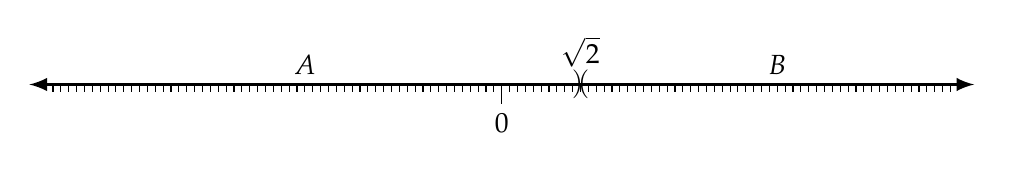
\begin{tikzpicture}
        \draw[latex-latex, very thick] (-6, 0) -- (6,0) node[anchor=south] {$\QQ$};
        \draw[] (0, 0) -- (0, -0.25) node[anchor=north] {0};
        \foreach \i in {-5.7,-5.6,...,5.7}{ 
        \draw[] (\i,0) -- (\i,-0.1);
        }
        \draw[] (1,0.1) node[anchor=south] {$\sqrt{2}$};
        \draw[] (0.96,0) node[] {$)$};
        \draw[] (1.04,0) node[] {$($};
        \draw[] (-2.5, 0) node[anchor=south] {$A$};
        \draw[] (3.5, 0) node[anchor=south] {$B$};
    \end{tikzpicture}
    \caption{Visualization of sets $A$ and $B$. We note that $\sqrt{2}$ has not been defined in our formalism yet, but from our prior mathematical intuition it would be what goes in the "hole" of the rationals.}
    \label{fig1}
\end{figure}

\noindent For the proof of this statement, we consider playing a 2 person game. One person is $\forall$, one person is $\exists$, and we consider if one person has a winning strategy. $\forall$ goes first, and then $\exists$ goes next, having seen the choice that $\forall$ has made. Then, we check if indeed $p < q$. If $p < q$, then $\exists$ wins. If $p \not< q$, then $\forall$ wins. 

\begin{nproof}
    Let $p \in A$. Then, let $q = \frac{2p + 2}{2 + p}$. Since $p \in \QQ$, it follows that $2p + 2 \in \QQ$ and $2 + p \in \QQ$ so $q \in \QQ$. Furthermore, we have that $2p + 2 > 0$ and $2 + p > 0$, so $q > 0$. We also have that:
    \[q^2 = \frac{(2p+2)^2}{(2+p)^2} = 2 + \frac{2(p^2 - 2)}{(p+2)^2} < 2\]
    Where the inequality follows from the fact that $p^2 < 2$ and hence $(p^2 - 2) < 0$. It therefore follows that $q \in A$. Finally, we have that:
    \[q = p + \frac{2-p^2}{2+p} > p\]
    so $q > p$, completing the proof of the first part of the claim. The second part is left as an exercise (we note that the same $q$ can be used). \qed
\end{nproof}

\noindent The number $q = \frac{2p+ 2}{2 + p}$ seems to be pulled out of a hat, but actually comes from a fairly geometric picture (the secant method of approximating roots). Discussion on this topic can be found here: \\ \texttt{https://math.stackexchange.com/questions/141774/choice-of-q-in-baby-rudins-example-1-1}.

\subsection{Ordered Sets}
Over the next couple sections, we will be discussing certain properties of sets that will give us a better understanding of the real numbers, and allow us to construct them.

\setcounter{rudin}{4}

\begin{definition}{Order}{1.5}
    An \textbf{order} $<$ on a set $S$ is a relation with the following properties:
    \begin{enumerate}[(i)]
        \item For every pair $x, y \in S$, exactly one of $x < y$, $x = y$, or $y < x$ is true. 
        \item For $x, y, z \in S$, if $x < y$ and $y < z$, then $x < z$. 
    \end{enumerate}
    A point on notation; We note that $x > y$ means $y < x$, and $x \leq y$ means $x < y$ or $x = y$. 
\end{definition}

\begin{definition}{Ordered Sets}{1.6}
    An \textbf{ordered set} is a pair $(S, <)$. We may write just $S$ if the order can be inferred by the context.
\end{definition}
\noindent A familiar (and useful) set of examples is $S = \NN$ or $S = \ZZ$ or $S = \QQ$. For these three sets, we have that $x < y$ if $y-x$ is positive. For another example, consider the set $S$ of english words; then the order $<$ can be the dictionary/lexographic order. 

\begin{definition}{Upper \& Lower Bounds}{1.7}
    Let $S$ be an ordered set and $E \subset S$ (note that here, $E \subset S$ is a non-strict subset, and $E \subsetneq S$ is a strict subset). $E$ is \textbf{bounded above} if there exists an element $\beta \in S$ such that $\forall x \in E$, $x \leq \beta$. Any such $\beta$ is an \textbf{upper bound} of $E$. Similarly, we say that $E$ is \textbf{bounded below} if there exists an element $\alpha \in S$ such that $\forall x \in E$, $\alpha \leq x$. In this case, $\alpha$ is a \textbf{lower bound} of $E$.
\end{definition}
\noindent As an example, one can take $S = \QQ$, $E = A = \set{p \in \QQ: p > 0, p^2 > 2}$ (as in Example \ref{exam:1.1b}). Here, $E$ is bounded above, with $\beta = 2$ as one possible upper bound. to see this is the case, consider that if $p \in E$:
\[2 - p = \frac{4 - p^2}{2+p} > \frac{4-2}{2+p} > 0\]
\noindent However, if we take $S = A$, $E = A$, then $E$ is not bounded above as we saw in the example. There is no upper bound of $A$ in $A$. In general, this example reveals the subtle point that "the upper bound of a set" is ill-defined; we need to specify $E \subset S$. 

\subsection{The Least Upper Bound Property}
\begin{definition}{Least Upper Bound \& Greatest Lower Bound}{1.8}
    Let $S$ be an ordered set, and let $E \subset S$ with $E$ bounded above. If $\exists \alpha \in S$ such that:
    \begin{enumerate}[(i)]
        \item $\alpha$ is an upper bound for $E$
        \item If $\gamma < \alpha$, then $\gamma$ is not an upper bound for $E$
    \end{enumerate} 
    The $\alpha$ is the \textbf{least upper bound}, or \textbf{supermum} of $E$. This can be denoted as $\alpha = \sup(E)$. Analogously, the \textbf{greatest lower bound}, or \textbf{infimum} of E (denoted $\alpha = \inf(E)$) is an element $\alpha \in S$ (if it exists) such that:
    \begin{enumerate}[(i)]
        \item $\alpha$ is a lower bound for $E$
        \item If $\gamma > \alpha$, then $\gamma$ is not an upper bound of $E$. 
    \end{enumerate}
\end{definition}

\begin{ntheorem}{Uniqueness of supremum/infimum}
    If the supremum/infimum of $E \subset S$ exist, they are unique.
\end{ntheorem}
\begin{nproof}
        Let $E \subset S$. Suppose that there exist $\alpha_1, \alpha_2$ such that $\alpha_1 = \sup(E)$ and $\alpha_2 = \sup(E)$. If $\alpha_1 < \alpha_2$, as $\alpha_1$ is an upper bound of $E$, this contradicts the fact that $\alpha_2$ is the least upper bound of $E$. We reach an identical contradiction if $\alpha_2 < \alpha_1$. Therefore we conclude that $\alpha_1 = \alpha_2$ and the supremum of $E$ is unique (if it exists). The proof for the infimum is analogous. \qed
\end{nproof}

\begin{ntheorem}{Equivalence of maximum and supremum}
    If $E \subset S$ has a maximum element $\alpha$ (that is, an element such that $x < \alpha$ for all $x \in E$) then $\alpha = \sup(E)$. Similarly, if $E$ has a minimum element $\alpha$, then $\alpha = \inf(E)$.
\end{ntheorem}

\begin{nproof}
    Let $E \subset S$ and $\alpha = \max(E)$. By definition $\alpha$ is an upper bound of $E$, and if $x < \alpha$ for some $x \in E$ then $x$ is not an upper bound of $E$ as it is not greater than $\alpha \in E$. The claim follows (with an identical proof for the minimum). \qed
\end{nproof}

\begin{example}{}{1.9}
    \begin{enumerate}
        \item Consider again the sets $A, B \subset \QQ$ from example \ref{exam:1.1b}. $A$ is bounded above by any element in $B$, and the upper bounds of $A$ are exactly the elements of $B$. Since $B$ has no smallest member, $A$ does not have a least upper bound in $\QQ$.
        \item Let $E_1, E_2 \subset \QQ$ such that $E_1 = \set{r: \QQ, r < 0}$ and $E_2 = \set{r: \QQ, r \leq 0}$. Then $\sup(E_1) = \sup(E_2) = 0$. Note that this example shows that the supremum can either be contained or not contained in the set; $0 \notin E_1$ but $0 \in E_2$. 
        \item Let $E \subset \QQ$ such that $E = \set{\frac{1}{n}: n \in \NN}$. Then $\sup(E) = 1$ and $\inf(E) = 0$. This is proven below. 
    \end{enumerate}
\end{example}
\begin{nproof}
    $\sup(E) = 1$ immediately follows from the equivalence of the maximum and supremum as proven above. To see that $\inf(E) = 0$, first note that $0$ is a lower bound for $E$ as all of the elements of $E$ are positive. To see that it is the lower bound, take any $x > 0$. Then, we have that for any $n > \frac{1}{x}$, $\frac{1}{n} < x$ and hence $x$ is not an upper bound of $E$. This proves the claim. \qed
\end{nproof}

\begin{definition}{The LUB/GUB Property}{1.10}
    An ordered set $S$ has the \textbf{least upper bound property} if for every $E \subset S$, if $E \neq \emptyset$ and $E$ is bounded above, then $E$ has a least upper bound (that is, $\sup(E)$ exists in $S$). Similarly, an ordered set $S$ has the \textbf{greatest lower bound property} if for every $E \subset S$, if $E \neq \emptyset$ and $E$ is bounded below, then $E$ has a greatest lower bound.
\end{definition}
\noindent We will show in the next theorem that these properties are actually equivalent; before then, we briefly consider two examples.
\begin{nexample}{$\ZZ$ and $\QQ$}
    $\ZZ$ has the least upper bound property, while $\QQ$ does not. 
\end{nexample}
\begin{nproof}
    For the first claim, consider any nonempty $E \subset \ZZ$ that is bounded above. Choose any $x \in E$. Since $\ZZ$ is bounded above, there exist finitely many elements that are greater than $x$. Take the maximum of these finitely many elements. This maximum is also the maximum of $E$, so it is the supremum of $E$. Therefore $\ZZ$ has the LUB property as claimed.
    
    The second claim immediately follows from Example \ref{exam:1.9}(a). \qed
\end{nproof}

\begin{theorem}{Equivalence of LUB/GUB properties}{1.11}
    Let $S$ be an ordered set. Then $S$ has the LUB property if and only if it has the GUB property. 
\end{theorem}
\begin{nproof}
    $\boxed{\implies}$ Let $S$ be an ordered set with the LUB property. Let $E \subset S$ with $E \neq \emptyset$, with $E$ bounded below. Let $L = \set{x \in S: x\text{ is a lower bound of $E$.}}$. $L \neq \emptyset$ as $E$ is bounded below (and hence has at least one lower bound). If $y \in E$, then $y$ is an upper bound for $L$. Since $E$ is nonempty, $L$ is therefore bounded above. Since $S$ has the LUB property, then $\sup(L)$ must exist. Let us call this $\alpha$. Then, $\alpha \leq x\ \forall x \in E$ (as if $\gamma < \alpha$, then $\gamma$ is not an upper bound of $L$ and hence $\gamma \neq E$). Hence, $\alpha$ is a lower bound for $E$ and hence $\alpha \in L$. Since $\alpha = \sup(L)$ and $\alpha$ is an upper bound for $L$, we have that $\alpha \geq \gamma\ \forall \gamma \in L$. Thus, $\alpha = \inf(E)$. 

    $\boxed{\impliedby}$ Left as an exercise. \qed
\end{nproof}

\subsection{Fields and Ordered Fields}
\begin{definition}{Fields}{1.12}
    A \textbf{field} $F$ is a set with two binary operations, $+$ and $\cdot$ (addition and multiplication) such that the following axioms are satisfied:
    \begin{enumerate}[start=1, label={(A\arabic*):}]
    \item If $x, y \in F$, then $x + y \in F$. (Closure under addition)
    \item $x + y = y + x$ for all $x, y \in F$. (Commutativity of addition)
    \item $(x+y) + z = x + (y + z)$ for all $x, y, z \in F$. (Associativity of addition)
    \item $\exists 0 \in F$ such that $\forall x \in F$, $0 + x = x$. (Additive identity)
    \item $\forall x \in F$, $\exists y$ such that $x + y = 0$. We can denote $y = -x$. (Additive inverse)
    \end{enumerate}
    \begin{enumerate}[start=1, label={(M\arabic*):}]
        \item If $x, y \in F$, then $x\cdot y\in F$. (Closure under multiplication)
        \item $x \cdot y = y \cdot x$ for all $x, y \in F$.
        \item $(x\cdot y)\cdot z = x \cdot (y \cdot z)$ for all $x, y, z \in F$. (Associativity under multiplication)
        \item $\exists 1 \in F$ such that $1 \neq 0$ and $\forall x \in F$, $1 \cdot x = x$. (Multiplicative identity)
        \item $\forall x \in F$, exists $y \in F$ such that $x \cdot y = 1$. We can denote $y = \frac{1}{x}$. (Multiplicative inverse)
    \end{enumerate}
    (D): $x \cdot (y + z) = x \cdot y + x \cdot z$, $\forall x, y, z \in F$. (Distributive law)
\end{definition}
\noindent Note that A3/M3 show that $x + y + z$ and $x\cdot y\cdot z$ are well defined in a mathematical sense; however, associativity may not hold for computers that do math with finite precision! 
\begin{ntheorem}{Uniqueness of Identities and Inverses}
    The additive/multiplicative identities given by (A4)/(M4) and the additive/multiplicative inverses given by (A5)/(M5) are unique. 
\end{ntheorem}
\begin{nproof}
    Let $F$ be an ordered field. Suppose that there exist $0_1, 0_2 \in F$ such that $0_1 + x= x$ and $0_2 + x = x$ for all $x \in F$. We then have that:
    \begin{align*}
        0_1 + 0_2 &= 0_1 + 0_2
        \\ 0_1 + 0_2 &= 0_2 + 0_1 & \text{(A2)}
        \\ 0_2 &= 0_1 & \text{(Property of additive identity)}
    \end{align*}
    Which shows that the additive identity is unique. The remaining proofs are left as an exercise. \qed
\end{nproof}
\noindent Some easy (and familiar) consequences of the field axioms can be found in Rudin 1.14-1.16. Instead of repeating those here, we will discuss some examples. 

The rationals form a field (under the usual notions of addition/multiplication), but the integers do not, as there are no multiplicative inverses (e.g. there exists no integer $x \in \ZZ$ such that $2\cdot x = 1$). The simplest example of a field is $F = \set{0, 1}$, with the relations:
\begin{align*}
    0 + 0 = 0\quad 0\cdot0 = 1
    \\ 0 + 1 = 0 \quad 0 \cdot 1 = 0
    \\ 1 + 1 = 0 \quad 1 \cdot 1 = 1
\end{align*}
This field is often called $\mathbb{F}_2$ or $F_2$, and is useful in computer science (where bits can take on two states, 0 or 1). As a slight tangent, a byte (8 bits) can be considered an element of an 8-dimensional vector space over the field $\mathbb{F}_2$, where $+$ would be the XOR operator and $\cdot$ would be the AND operation. 

A generalization of the above example is $\mathbb{F}_p$ or $F_p$, for a prime number $p$. This field would consist of the elements $0, 1, \ldots, p-1$. The addition and multiplication are carried out mod $p$. An interesting result is that in general, finite fields must have cardinality of some prime power. 

Note that a field cannot have a single element; the field axioms (A4) and (M4) require the existence of distinct additive and multiplicative identities, which a singleton set cannot satisfy. 

Although algebra is not the focus of this course, it may be interesting to briefly think about sets with less structure than a field. We start by considering a group. 

\phantom{i}

\noindent A \textbf{group} $G$ is a set with a binary operation $(a,b) \mapsto a\cdot b$ such that the following axioms are satisfied:
\begin{enumerate}[start=1, label={(M\arabic*):}]
    \item If $a, b \in G$, then $a\cdot b \in G$ (Closure)
    \stepcounter{enumi}
    \item For $a, b, c \in G$, $(a\cdot b)\cdot c = a\cdot(b\cdot c)$ (Associativity)
    \item There exists $1 \in G$ such that $\forall x \in G$, $1 \cdot x = x$. (Identity)
    \item $\forall x \in G$, there exists $y \in G$ such that $x \cdot y = 1$. (Inverse) 
\end{enumerate}

We note that $\ZZ$ is a group under addition, but not under multiplication (due to lack of multiplicative inverses). We can also consider the set of 2x2 matrices with integer entries:
\[G = \set{\m{a & b \\ c & d}: a, b, c, d \in \ZZ}\]
$G$ is again a group under matrix addition, but not under matrix multiplication (as not every matrix in $G$ is invertible). If we restricted $G$ to be the set of $2\times 2$ invertible matrices, in this case it could form a group under matrix multiplication. A set with slightly more structure than a group (though not quite as structured as a field) is a ring:
\newpage 
\noindent A \textbf{ring} $R$ is a set with two binary operations $(a,b) \mapsto a + b$ and $(a, b) \mapsto a \cdot b$ such that the following axioms are satisfied:
\begin{enumerate}[start=1, label={(A\arabic*):}]
    \item If $x, y \in R$, then $x + y \in R$. (Closure under addition)
    \item $x + y = y + x$ for all $x, y \in R$. (Commutativity of addition)
    \item $(x+y) + z = x + (y + z)$ for all $x, y, z \in R$. (Associativity of addition)
    \item $\exists 0 \in R$ such that $\forall x \in R$, $0 + x = x$. (Additive identity)
    \item $\forall x \in R$, $\exists y$ such that $x + y = 0$. We can denote $y = -x$. (Additive inverse)
    \end{enumerate}
    \begin{enumerate}[start=1, label={(M\arabic*):}]
        \item If $x, y \in R$, then $x\cdot y\in R$. (Closure under multiplication)
        \stepcounter{enumi}
        \item $(x\cdot y)\cdot z = x \cdot (y \cdot z)$ for all $x, y, z \in R$. (Associativity under multiplication)
        \item $\exists 1 \in R$ such that $1 \neq 0$ and $\forall x \in R$, $1 \cdot x = x$. (Multiplicative identity)
    \end{enumerate}
    \begin{enumerate}[start=1, label={(D\arabic*):}]
        \item $x \cdot (y + z) = x \cdot y + x \cdot z$, $\forall x, y, z \in R$. (Left distributivity)
        \item $(y + z) \cdot x = y \cdot x + z \cdot x$, $\forall x, y, z \in R$. (Right distributivity)
    \end{enumerate}

\noindent Rings have the same axioms as fields under addition, but multiplication is not necessarily commutative (this is why an additional distributivity axiom is added), and multiplicative inverses are not required. We note that $\ZZ$ and $G$ are both rings under their respective operations of addition and multiplication. 

For the remainder of this course, we will really only be discussing fields; however, they will be the objects of interest in abstract algebra courses!

\setcounter{rudin}{16}
\begin{definition}{Ordered Field}{1.13}
    An \textbf{Ordered field} is a field $F$ that is also an ordered set, such that the following axioms are satisfied:
    \begin{enumerate}[(i)]
        \item If $x, y, z \in F$ and $y < z$, then $x + y < x + z$.
        \item If $x, y \in F$ and $x > 0, y > 0$, then $x\cdot y > 0$.
    \end{enumerate}
\end{definition}
\noindent Some properties of ordered fields are discussed in Rudin 1.18. We will again refer the reader to the discussion in the textbook for these properties, and here consider some examples.

$\QQ$ is an ordered field, with the familiar order of $a > b$ if $a - b > 0$. A question may arise if $\mathbb{F}_2$ is an ordered field. A priori fields do not have order, but is it possible to impose an order on this set such that it is an ordered field? The answer turns out to be no.

\begin{proof}
    It suffices to show that both possible orderings leads to a contradiction. Suppose $0 < 1$. Then, $1 = 0 + 1 < 1 + 1 = 0$ which is a contradiction. Suppose instead that $1 < 0$. Then, $0 = 1 + 1 < 1 + 0 = 1$ which again is a contradiction.
\end{proof}

\stepcounter{rudin}

\begin{theorem}{Existence of $\RR$}{1.19}
    There exists an ordered field $\RR$ which has the LUB property and contains $\QQ$ as a subfield. 
\end{theorem}
\noindent What does it mean for $\QQ$ to be a subfield? It means that there exists an injective function $\QQ \mapsto \RR$ that respects the properties of an ordered field.

This field $\RR$ happens to be exactly the set of real numbers we are familiar with. However, a natural question is ``what does it mean that there exsits a field?" It turns out that we can define the reals based on the definitions we have made already. One further question might be that could there not exists several fields with the above property; however, taking the appropriate view, we will find that there is a unqiue such field. 

\subsection{Consequences of the LUB Property}
We will use the least upper bound property and the fact that $\RR$ has $\QQ$ as a subfield to derive its properties.
\begin{theorem}{Archimedian Property, Density of the Rationals/Irrationals}{1.20}
    \begin{enumerate}
        \item If $x, y \in \RR$ and $x > 0$, then $\exists n \in \NN$ such that $nx > y$.
        \item If $x, y \in \RR$, and $x < y$, then $\exists p \in \QQ$ such that $x < p < y$. ($\QQ$ is dense in $\RR$)
        \item If $x, y \in \RR$, and $x < y$, then $\exists \alpha \in \RR \setminus \QQ$ such that $x < \alpha < y$. ($\RR\setminus\QQ$ is dense in $\RR$)
    \end{enumerate}
\end{theorem}

\begin{nproof}
    (a) Let $A = \set{nx: n \in \NN}$. Suppose for the sake of contradiction that the conclusion was false; then $y$ is an upper bound of $A$. Then, $\alpha = \sup(A)$ exists by the LUB property of $\RR$. Since $x > 0$, we then have that $\alpha - x < \alpha$ by the property of an ordered field. Hence, $\alpha - x$ is not an upper bound for $A$. Therefore, there exists some $m \in \NN$ such that $mx > \alpha - x$. It then follows that $(m+1)x > \alpha$. We therefore have found $m+1 = k \in \NN$ such that $kx > \alpha$, contradicting $\alpha$ being the least upper bound of $A$. \qed
\end{nproof}

\noindent In order to prove (b) and (c), we first prove a stronger version of (a):

\begin{nlemma}{}
    If $x, y \in \RR$ and $x > 0$, then there exists $n \in \ZZ$ such that $(n-1)x \leq y < nx$. 
\end{nlemma}
\begin{nproof}
    Suppose $y \geq 0$. Let $A = \set{m \in \NN: y < mx} \subset \NN$. By Theorem \ref{thm:1.20} (a), we have that $A \neq \emptyset$. Every non-empty subset of $\NN$ has a smallest element (to see this, let $x \in A$, and define $A' = \set{y \in A: y \leq x}$. This is finite and nonempty and so has a smallest element, and the minimum element of this set will also be a lower bound and hence the minimum element of all of $A$), so let $n = \min(A)$. The claim holds for this $n$.
    The case for $y < 0$ is left as an exercise. \qed
\end{nproof}
\begin{nproof}
    (b) Since $y - x > 0$, by (a), $\exists n \in \NN$ such that $1 < n(y-x)$. Furthermore, by the Lemma we have that $\exists m \in \ZZ$ such that $m - 1 \leq nx < m$ and hence $m \leq nx + 1$. From these inequalities we obtain that $nx < m \leq nx + 1 < ny$, and therefore $x < \frac{m}{n} < y$ for some $m \in \ZZ$, $n \in \NN$. \qed
\end{nproof}
\noindent For the proof of part (c), we will use the result of Theorem \ref{thm:1.21} from the next section, specifically that there exists $s \in \RR \setminus \QQ$ such that $s > 0$ and $s^2 = 2$. We will call this $\sqrt{2}$.
\begin{nproof}
    (c) First, we have that $\sqrt{2} < 2$ as if $\sqrt{2} = 2$ then $(\sqrt{2})^2 = 2 = 2^2 = 4$ which is a contradiction, and if $\sqrt{2} > 2$ then $2 = \sqrt{2}\cdot \sqrt{2} > 2\cdot 2 = 4$ by Rudin 1.18 which is yet again a contradiction. Thus, $\frac{\sqrt{2}}{2} < 1$. 
    
    Let $x, y \in \RR$ such that $x < y$. By Theorem \ref{thm:1.20}(b), there exists $p, q \in \QQ$ such that $x < p < q < y$. Let $\alpha = p + \frac{\sqrt{2}}{2}(q - p)$. Then, we have that $p  <\alpha < p + 1(q-p) < q$ and hence $x < p < \alpha < q < y$.

    If $\alpha \in \QQ$, then $\sqrt{2} = 2\left(\frac{\alpha-p}{q-p}\right) \in \QQ$, which is a contradiction, so it follows that $\alpha \in \RR \setminus \QQ$. \qed
\end{nproof}

\subsection{Integer Roots of the Reals}
In this section, we will prove that $\sqrt{2}$ exists and is an irrational number, but we will not use the fact that $\RR \setminus \QQ$ is dense in $\RR$; this would of course be circular reasoning. The more general idea will be to prove that for any $n \in \NN$, there exists $y \in \RR$ such that $y = x^{1/n}$. Before this, we prove a lemma.
\begin{nlemma}{}
    If $0 < a < b$ and $n \in \NN$, then $0 < b^n - a^n \leq nb^{n-1}(b-a)$
\end{nlemma}
\noindent Note that a "Calculus proof" of this Lemma would be to let $f(x) = x^n$, and then
\[f(b) - f(a) = f'(c)(b-a) = nc^{n-1}(b-a) \leq nb^{n-1}(b-a)\]
Where we invoke the mean value theorem. But this obviously doesn't work as we have neither defined a derivative nor proven the mean value theorem. A proper proof would be:
\begin{nproof}
    Let $0 < a < b$. Then, we may factor $b^n - a^n$ such that:
    \[b^n - a^n = (b-a)(b^{n-1} + ab^{n-2} + a^2b^{n-3} + \ldots + a^{n-2}b + a^{n-1})\]
    The second factor is a sum of $n$ terms, each positive, and in between $0$ and $b^{n-1}$. ThereforE:
    \[b^n - a^n \leq nb^{n-1}(b-a)\]
    which proves the claim. \qed
\end{nproof}
\noindent We will now state the theorem formally:
\begin{theorem}{Roots of real numbers}{1.21}
    Let $x \in \RR$, $x > 0$, and $n \in \NN$. Then, there exists a unique $y \in \RR$ such that $y > 0$ and $y^n = x$. 
\end{theorem}
\noindent Note that somewhere in the proof, we will use the fact that $y \in \RR$; this statement doesn't hold for rationals (see Example \ref{exam:1.1a}) so some property of the reals must come into play somewhere.
\begin{nproof}
    If $n = 1$, then the unique solution is $y = x$; we may therefore assume that $n \geq 2$.
    \\ \textbf{Uniqueness:} Suppose there exist two distinct numbers $y_1, y_2$ with $y_1 > 0, y_2 > 0$, and $y_1^n = y_2^n = x$. WLOG, suppose $0 < y_1 < y_2$. We then have that $0 < y_1^n < y_2^n$ which is a contradiction. 
    \\ \textbf{Existence:} We prove existence in three steps.
    \begin{enumerate}[1.]
        \item We show that $E \neq \emptyset$. Let $E = \set{t \in \RR: t > 0, t^n < x}$. If $x < 1$, then $x^n < x$, so $x \in E$. If $x \geq 1$, then $\left(\frac{1}{2}\right)^n < \frac{1}{2} < x$, so $\frac{1}{2} \in E$. Therefore, $E \neq \emptyset$.
        \item We show that $E$ is bounded above and has a supremum in $\RR$. If $t > 1 + x$, then it follows that $t^n > t > x$, so $t \neq E$. Hence, $1 + x$ is an upper bound of $E$. By Theorem \ref{thm:1.19} (the LUB property of $\RR$), it follows that $\sup(E) \in \RR$ exists. 
        \item We show that $y = \sup(E)$ satisfies $y^n = x$. As $\RR$ is an ordered field, one of $y^n < x$, $y^n = x$, or $y^n > x$ must be true; we show that the first and third are impossible.
        \begin{enumerate}
            \item Suppose $y^n < x$. We will obtain a contradiction by finding $h > 0$ such that $(y+h)^n < x$. (Why is this a contradiction? $y+ h > y$, so if $(y+h)^n < x$, then $y + h \in E$, contradicting the fact that $y + h$ would be an upper bound of $E$). WLOG, suppose that $h < 1$. By the above Lemma, we have that:
            \[(y+h)^n - y^n \leq n(y+h)^{n-1}h \leq n(y+1)^{n-1}h\]
            By choosing $h$ sufficiently small, that is:
            \[h < \min\set{1, \frac{x-y^n}{n(y+1)^{n-1}}}\]
            Then $n(y+1)^{n-1}h < x^n - y^n$ from which it follows that $(y+h)^n - y^n < x^n - y^n$ and so $y+h < x$, which is the desired contradiction.
            \item Suppose $y^n > x$. We will obtain a contradivction by finding $h > 0$ such that $(y-h)^n > x$. If this is true, then $y-h$ is an upper bound for $E$, contradicting the fact that $y$ is the least upper bound for $E$. WLOG suppose that $h < 0$. Again applying the Lemma, we have that:
            \[y^n - (y-h)^n \leq ny^{n-1}h\]
            By choosing $h$ sufficiently small, that is:
            \[h < \min\set{1, \frac{y^n-x}{ny^{n-1}}}\]
            It then follows that:
            \[y^n - (y-h)^n \leq ny^{n-1}h < y^n - x\]
            and hence $(y-h)^n > x$, which is the desired contradiction. \qed
        \end{enumerate} 
    \end{enumerate}
\end{nproof}
\subsection{Construction of the Reals}
Theorem \ref{thm:1.19} says that there exists an ordered field that contains $\QQ$ as a subfield. We now go about proving this statement. The construction is fairly technical and hence will be carried out in multiple steps. Some of the steps are left as exercises (one can refer to Rudin for the fully complete construction).

\begin{nblank}{Step 1: Defining the elements of $\RR$}
    The members of $\RR$ will be proper subsets of $\QQ$, called cuts. $\RR = \set{\text{all cuts}}$. 
    \begin{ndef}{Cuts}
        A \textbf{cut} is a proper subset $\alpha \subsetneq \QQ$ with the three properties:
        \begin{enumerate}[(I)]
            \item $\alpha \neq \emptyset$
            \item If $p \in \alpha$, then $q \in \alpha \; \forall q < p$. 
            \item If $p \in \alpha$, then $\exists r \in \alpha$ such that $p < r$. 
        \end{enumerate}
    \end{ndef}
\end{nblank}
\begin{figure}[htbp]
    \centering
    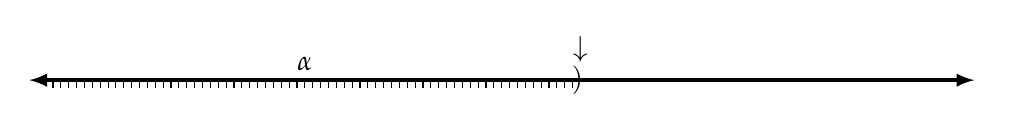
\begin{tikzpicture}
        \draw[latex-latex, very thick] (-6, 0) -- (6,0) node[anchor=south] {$\QQ$};
        \foreach \i in {-5.7,-5.6,...,0.9}{ 
        \draw[] (\i,0) -- (\i,-0.1);
        }
        \draw[] (1,0.1) node[anchor=south] {$\downarrow$};
        \draw[] (0.96,0) node[] {$)$};
        \draw[] (-2.5, 0) node[anchor=south] {$\alpha$};
    \end{tikzpicture}
    \caption{Visualization of a cut $\alpha$. The real number being described of this cut can be thought of as the number at the right boundary (the arrow).}
    \label{fig2} 
\end{figure}
\noindent In a sense, a cut gives us a way of discussing the real numbers (in the way we are familiar with them already) without referring to them directly; much like we could formally define/refer to rationals as equivalence classes of ordered pairs.  

\noindent As a note, we could very well define cuts to be bounded below rather than above, and the following construction would still work out.

\begin{nblank}{Step 2: $\RR$ is an ordered set}
    We define $\alpha < \beta$ to mean $\alpha \subsetneq \beta$. We show that this makes $\RR$ into an ordered set. First checking transitivity, we have that if $\alpha < \beta$ and $\beta < \gamma$ then $\alpha < \gamma$ by the fact that set inclusion is transitive. Furthermore, at most one of $\alpha < \beta$, $\alpha = \beta$, and $\beta < \alpha$ hold; to see this is the case, suppose the first two fail. Then, $\alpha \nsubseteq \beta$. Hence, $\exists p \in \alpha$ with $p \notin \beta$. If $q \in \beta$, $q < p$  and hence $q \in \alpha$ by (II), so $\beta \subset \alpha$, and since $\beta \neq \alpha$ it follows that $\beta \subsetneq \alpha$. 
\end{nblank}

\begin{nblank}{Step 3: $\RR$ has the LUB property}
    We show that $\RR$ has the LUB property. To see this is the case, let $A \subset \RR$ with $A \neq \emptyset$, and suppose that there exists $\beta \in \RR$ that is an upper bound for $A$. We will now define $\gamma = \bigcup_{\alpha \in A}\alpha$ and prove that $\gamma \in \RR$ and $\gamma = \sup A$ (hence $A$ has a supremum and $\RR$ has the LUB property).

    Since $A \neq \emptyset$, $\exists \alpha_0 \in A$, and since $\alpha_0 \neq \emptyset$ (as it is a cut) and $\alpha \subset \gamma$, it follows that $\gamma \neq \emptyset$. Next, we have that $\gamma \subset \beta$, since $\alpha \subset \beta$ for every $\alpha \in A$, and hence $\gamma \neq \QQ$, that is, $\gamma \subsetneq \QQ$. Hence $\gamma$ satisfies property (I) of a cut. 

    Take $p \in \gamma$. Then $p \in \alpha_1$ for some $\alpha_1 \in A$. If $q < p$, then $q \in \alpha$ (as $\alpha$ is a cut) so $q \in \gamma$, satisfying property (II).

    Next, choose $r \in \alpha_1$ such that $r > p$, then $r \in \gamma$ (as $\alpha_1 \subset \gamma$) and hence $\gamma$ satisfies property (III). Hence $\gamma$ is a cut, and $\gamma \in \RR$.

    Finally, we show that $\gamma = \sup A$. Clearly, $\alpha \leq \gamma$ for all $\alpha \in A$, as $\gamma = \bigcup_{\alpha \in A}\alpha$, so $\gamma$ is an upper boun dof $A$. To show that it is the least upper bound, let $\delta < \gamma$ be a cut. Then, $\exists s \in \gamma$ such that $s \notin \delta$. Therefore, $\exists \alpha_2 \in A$ such that $s \in \alpha_2$; hence $\delta < \alpha_2$, so $\delta$ is not an upper bound for $A$, giving the desired result. 
\end{nblank}

\begin{nblank}{Step 4: Addition on $\RR$}
    \begin{ndef}{Addition}
        If $\alpha, \beta \in \RR$, we define $\alpha + \beta = \set{s + t: s \in \alpha, t \in \beta}$. Showing that this is a cut is left as an exercise.
    \end{ndef}
    \begin{ndef}{Zero}
        $0^* = \set{s \in \QQ}$. Showing that this is a cut is left as an exercise.
    \end{ndef}

    We leave it as an exercise to show that the addition axioms (A1)-(A5) of a field are satisfied under this definition of addition on $\RR$, with the 0 element as $0^*$ defined above.
\end{nblank}

\begin{nblank}{Step 5: $\RR$ satisfies the Ordered Field Property (i)}
    We verify that if $\alpha, \beta, \gamma \in \RR$ and $\beta < \gamma$, then $\alpha + \beta < \alpha + \gamma$. 

    For every $s \in \alpha, t \in \beta$, we have that $t \in \gamma$ as $\beta$ is a subset of $\gamma$ by the definition of order on $\RR$. Hence, $s + t \in \alpha + \beta$ implies $s + t \in \alpha + \gamma$. Therefore, $\alpha + \beta \subseteq \alpha + \gamma$ and hence $\alpha + \beta \leq \alpha + \gamma$. 

    We are then left to check that $\alpha + \beta \neq \alpha + \gamma$. To see that this is the case, if $\alpha + \beta = \alpha + \gamma$, then $\beta = \alpha + \beta - \alpha = \alpha + \gamma - \alpha = \gamma$ by the field axioms for addition. Therefore we obtain that $\beta = \gamma$, contradicting that $\beta < \gamma$. Hence the claim is proven.

    As a remark, note that $0^* < \alpha \iff -\alpha < 0^*$.
\end{nblank}
\noindent Next we will define multiplication on $\RR$. A first attempt would be $\alpha \cdot \beta = \set{s \cdot t: s\in \alpha, t \in \beta}$. However, this definition is incosistent with negative numbers from what we require multiplication to accomplish. $-1 \cdot -1$ would fail to be a cut (it would not contain any negative numbers and hence fail criteria (II)) and $-1 \cdot 1$ would yield the entirety of the rationals (again not a cut!)

\begin{nblank}{Step 6: Positive Multiplication on $\RR$}
    \begin{ndef}{Positive Reals}
        We define $\RR^+ = \set{\alpha \in \RR: \alpha > 0^*}$
    \end{ndef}
    \begin{ndef}{Multiplication of Positive Reals}
        If $\alpha, \beta \in \RR^+$, we define $\alpha \cdot \beta = \set{r \cdot s: r \in \alpha, r> 0, s \in \beta, s > 0} \cup \set{t \in \QQ, t \leq 0}$. Equivalently, $\alpha \cdot \beta = \set{p \in \QQ:  \leq r \cdot s: r \in \alpha, r > 0, s \in \beta, s > 0}$. We leave it as an exercise to show that $\alpha \cdot \beta \in \RR$, and moreover, $\alpha \cdot \beta \in \RR^+$. Showing this second fact proves ordered field property (ii).
    \end{ndef}
    \begin{ndef}{One}
        $1^* = \set{r \in \QQ: r < 1}$. We again leave showing $1^* \in \RR^+$ as an exercise. 
    \end{ndef}
\end{nblank}

\begin{nblank}{Step 7: Multiplication on all of $\RR$}
    \begin{ndef}{Multiplication by zero}
        $\alpha \cdot 0^* = 0^* = 0^* \cdot \alpha$
    \end{ndef}
    \begin{ndef}{Multiplication}
        We define general multiplication as below, where the $\cdot$ on the RHS represents the multiplication of positive reals as outlined in Step 5. 
        \begin{align*}
            \alpha \cdot \beta = 
            \begin{cases}
            (-\alpha)\cdot(-\beta) & \text{if $\alpha < 0^*$ and $\beta < 0^*$}
            \\ -\left((-\alpha)\cdot\beta\right) & \text{if $\alpha < 0^*$ and $\beta > 0^*$}
            \\ -\left(\alpha \cdot (-\beta)\right) & \text{if $\alpha > 0^*$ and $\beta < 0^*$}
            \end{cases}
        \end{align*}
    \end{ndef}
    We leave it as an exercise to show that the multiplicative axioms (M1)-(M5), as well as the distributive law (D) of a field are satisfied under this definition of multiplication on $\RR$. 
\end{nblank}
\noindent Up until this point, we have shown $\RR$ is an ordered field with the LUB property; we last check that it contains $\QQ$ as a subfield. Note that we do have to be a bit careful with what we mean here; $\RR$ does not literally contain $\QQ$; $\RR$ is indeed a set of proper subsets of $\QQ$. What we really mean is to associate every element of $\QQ$ to an element of $\RR$ such that the field structure is preserved. 
\begin{nblank}{Step 8: $\RR$ contains $\QQ$ as a subfield}
    For each $r \in \QQ$, associate the cut $r^* = \set{p \in \QQ, p < r^*}$. We then leave as an easy exercise to verify that $r^* < s^* \iff r < s$, $r^* + s^* = r + s$, and $r^*\cdot s^* = r\cdot s$. This concludes the construction of the reals. \qed
\end{nblank}
\noindent Note that later on in the course, we will construct the real numbers in a different fashion; by considering Cauchy sequences modulo an equivalence relation. Also note that from here on out, it will suffice to have the standard/traditional picture of a "real number" in mind (i.e. infinite decimal expansions) and we will not have to really think about the real numbers as cuts; this was just necessary for the formal construction.

\subsection{The Complex Field}
\setcounter{rudin}{23}
\begin{definition}{The Complex Numbers}{1.24}
    We define the set of \textbf{complex numbers} to be $\set{(a, b): a, b \in \RR}$, denoted by $\CC$. For $x = (a, b) \in \CC$ and $y = (c, d) \in \CC$, we write $x = y$ if and only if $a = c$ and $b = d$ (note that this is a very different notion of equality compared to the rationals). We define the zero element to be $(0, 0)$ and the one element to be $(1, 0)$. We define addition of complex numbers such that:
    \begin{align*}
        x + y = (a, b) + (c, d) = (a + c, b + d)
    \end{align*}
    And multiplication of complex numbers such that:
    \begin{align*}
        x\cdot y = (a, b)\cdot (c, d) = (ac - ba, ad + bc)
    \end{align*}
\end{definition}
\begin{theorem}{$\CC$ is a field}{1.25}
    The operations of $+$ and $\cdot$, as well as the zero/one elements defined above turn $\CC$ into a field. 
\end{theorem}
\begin{nproof}
    It suffices to verify the field axioms (A1)-(A5), (M1)-(M5), and (D) as discussed in \ref{def:1.12}. We will here show (M3), (M4), and (M5) and leave the rest as exercises. 
    \begin{enumerate}[start=3, label={(M\arabic*):}]
    \item Let $x, y, z \in \CC$. We show that $(x\cdot y)\cdot z = x \cdot (y \cdot z)$. Let $x = (a, b), y = (c, d)$, and $z = (e, f)$. We then have that:
    \begin{align*}
        (x\cdot y) \cdot z &= (ac - bd, ad + bc) \cdot (e, f)
        \\ &= ((ac-bd)e - (ad+bc)f, (ac-bd)f + (ad+bc)e)
    \end{align*}
    We also have that:
    \begin{align*}
        x \cdot(y\cdot z) &= (a, b)\cdot(ce - df, cf + de)
        \\ &= (a(ce-df) - b(cf+de), a(cf+de) + b(ce-df))
        \\ &= (ace - adf - bcf - bde, acf + ade + bce - bdf)
        \\ &= ((ac-bd)e - (ad+bc)f, (ac-bd)f + (ad+bc)e)
    \end{align*}
    So the claim is proven.
    \item $(a, b)(1, 0) = (a \cdot 1 - b \cdot 0, a \cdot 0 + b \cdot 1) = (a, b)$
    \item Let $x \in \CC$ such that $x \neq 0$. Then, $x = (a, b)$ where either $a \neq 0$ or $b \neq 0$ or both. Hence, $a^2 + b^2 > 0$. Then, let $\frac{1}{x} = (\frac{a}{a^2 + b^2}, -\frac{b}{a^2+b^2})$. We then have that:
    \begin{align*}
        x\frac{1}{x} &= (a, b)\left(\frac{a}{a^2 + b^2}, -\frac{b}{a^2+b^2}\right)
        \\ &= \left(a\frac{a}{a^2 + b^2} - b\left(-\frac{b}{a^2+b^2}\right), a\left(-\frac{b}{a^2+b^2}\right) + b\left(\frac{a}{a^2+b^2}\right)\right)
        \\ &= \left(\frac{a^2 +b^2}{a^2 + b^2}, -\frac{ab}{a^2+b^2} + \frac{ab}{a^2+b^2}\right)
        \\ &= (1, 0)
    \end{align*}
    Which proves the claim. \qed
    \end{enumerate}
\end{nproof}
\noindent Much like $\QQ$ was a subfield of $\RR$, $\RR$ is a subfield of $\CC$, and there exists a map $\phi$ from $\RR$ to $\CC$ that respects the field axioms, namely:
\begin{align*}
    \fullfunction{\phi}{\RR}{\CC}{x}{(x, 0)}
\end{align*}
The theorem below shows that $\phi$ preserves the field structure:
\begin{theorem}{}{1.26}
    For $a, b \in \RR$ we have that $(a, 0) + (b, 0) = (a + b, 0)$ and $(a, 0)(b, 0) = (ab, 0)$.
\end{theorem}
\begin{definition}{i}{1.27}
    $i = (0, 1)$. 
\end{definition}
\begin{theorem}{}{1.28}
    $i^2 = -1$. 
\end{theorem}
\begin{theorem}{}{1.29}
    If $a, b \in \RR$, then $(a, b) = a + bi$. 
\end{theorem}
\begin{nproof}
    Below are the trivial proofs for the above three theorems. 
    \begin{align*}
        (a, 0) + (b, 0) = (a + b, 0 + 0) = (a + b, 0)
        \\ (a, 0)\cdot(b, 0) = (a\cdot b - 0 \cdot 0, a \cdot 0 + 0 \cdot b) = (ab, 0)
        \\ i^2 = i\cdot i = (0, 1) \cdot (0, 1) = (-1, 0) = -1
        \\ a + bi = (a, 0) + b(0, 1) = (a, 0) + (0, b) = (a, b)
    \end{align*}
\end{nproof}
\noindent A slightly odd question may be to ask whether $\CC$ is a subfield of $\RR$, i.e. does there exist $\psi: \CC \mapsto \RR$ such that $\psi(a + b) = \psi(a) + \psi(b)$ and $\psi(a\cdot b) = \psi(a) \cdot \psi(b)$. As we will prove in Chapter 2, we do have that $\abs{\CC} = \abs{\RR^2} = \abs{\RR}$ (where $\abs{}$ denotes cardinality of the set, to be defined shortly), so there does exist a bijection (i.e. a function that is both injective/one-to-one and surjective/onto; we will define these terms precisely in the next chapter) between the two sets.

As a Lemma, we have that the only injective function $f: \QQ \mapsto \RR$ that satisfies $f(a+b) = f(a) + f(b)$ and $f(a\cdot b) = f(a)\cdot f(b)$ is $f(x) = x$. The proof of this is left as a homework problem (HW2). Therefore, it follows that the only injective function $g: \QQ \times \set{0} \mapsto \RR$ (where $\times$ denotes the Cartesian product) is given by $g((x, 0)) = x$. We now give a proof that $\CC$ is not a subfield of $\RR$. 

\begin{proof}
    Suppose then for the sake of contradiction that there exists an injective function $\psi: \QQ \times \set{0, 1} \mapsto \RR$. Such a function then must satisfy$\psi(i \cdot i) = \psi(-1) = -1$, and $\psi(i \cdot i) = \psi(i) \cdot \psi(i) = \psi((0, 1))\cdot \psi((0, 1)) = 0 \cdot 0 = 0$ which is a contradiction. Hence, no such injection exists from $\QQ \times \set{0, 1}$ to $\RR$ and hence no such injection could exist from $\CC$ ($\RR^2$) to $\RR$. Hence $\CC$ is not a subfield of $\RR$. 
\end{proof}



\begin{definition}{Real/Imaginary Parts and Complex Conjugates}{1.30}
Let $z = a + bi \in \CC$. Then, $\Re(z) = a$ is the \textbf{real part} of $z$ and $\Im(z) = b$ is the \textbf{imaginary part} of $z$. The \textbf{complex conjugate} of $z$, denoted by $\bar{z}$, is defined as $\bar{z} = a - bi$. 
\end{definition}

\begin{theorem}{Conjugate Properties}{1.31}
    Let $z, w \in \CC$. It then follows that:
    \begin{enumerate}
        \item $\overline{z + w} = \bar{z} + \bar{w}$.
        \item $\overline{zw} = \bar{z} \cdot \bar{w}$.
        \item $z + \bar{z} = 2\Re(z)$, $z - \bar{z} = 2i\Im(z)$.
        \item $z\bar{z}$ is real and positive (except when $z = 0$).
    \end{enumerate}
\end{theorem}

\begin{nproof}
    We prove (d). We have that:
    \begin{align*}
        z\bar{z} = (a + bi)(a-bi) = a^2 + b^2 
    \end{align*}
    $a^2 + b^2 \geq 0$, and $a^2 + b^2 = 0 \iff a = 0, b = 0$ which proves the claim. \qed
\end{nproof}

\begin{definition}{Absolute Value}{1.32}
    We define the \textbf{absolute value} $\abs{z}$ of a complex number $z$ as $\abs{z} = \sqrt{z\bar{z}}$. Note that if $a \in \RR$ and $z = (a, 0)$, then
    \begin{align*}
        \abs{z} = \sqrt{a^2} =
        \begin{cases}
            a & \text{if $a \geq 0$}
            \\ -a & \text{if $a < 0$}
        \end{cases}
    \end{align*}
    Hence if $a \in \RR$, we can define $\abs{a} = \abs{(a, 0)}$. 
\end{definition}

\begin{theorem}{Absolute Value Properties}{1.33}
    Let $z, w \in \CC$.
    \begin{enumerate}
        \item $\abs{z} \geq 0$, $\abs{z} = 0 \iff z = 0$. 
        \item $\abs{\bar{z}} = \abs{z}$.
        \item $\abs{z}\abs{w} = \abs{zw}$.
        \item $\abs{\Re(z)} \leq \abs{z}$, $\abs{\Im(z)} \leq \abs{z}$.
        \item $\abs{z + w} \leq \abs{z} + \abs{w}$.
    \end{enumerate}
\end{theorem}
\begin{nproof}
    We prove (d) and (e). Let $z, w \in \CC$, with $z = a + bi$. For (d) we have that $\Re(z) = a$, so \begin{align*}
        \abs{\Re(a)} = \sqrt{a^2} \leq \sqrt{a^2 + b^2} = \abs{z}
    \end{align*}
    And an equivalent proof follows for $\Im(z)$. For (e), we have that:
    \begin{align*}
        \abs{z + w}^2 &= (z + w)(\overline{z + w})
        \\ &= z\bar{z} + z\bar{w} + w\bar{z} + w\bar{w}
        \\ &= \abs{z}^2 + 2\Re(z\bar{w}) + \abs{w}^2
        \\ &\leq \abs{z}^2 + 2\abs{\Re(z\bar{w})} + \abs{y}^2 & \text{($\abs{x} > x$)}
        \\ &= \abs{z}^2 + 2\abs{z\bar{w}} + \abs{w}^2 & \text{(1.33(d))}
        \\ &= \abs{z}^2 + 2\abs{z}\abs{\bar{w}} + \abs{w}^2 & \text{(1.33(c))}
        \\ &= \abs{z}^2 + 2\abs{z}\abs{w} + \abs{w}^2 & \text{(1.33(b))}
        \\ &= (\abs{z} + \abs{w})^2
    \end{align*}
The claim follows by taking square roots on both sides. \qed
\end{nproof}



\subsection{The Cauchy-Shwartz Inequality}
Recall the summation notation:
\begin{align*}
    x_1 + x_2 + \ldots + x_n = \sum_{j=1}^{n}x_i
\end{align*}
\stepcounter{rudin}
\begin{theorem}{Cauchy-Shwartz Inequality}{1.35}
    Let $a_1, \ldots, a_n, b_1, \ldots, b_n \in \CC$. We then have that:
    \begin{align*}
        \abs{\sum_{j=1}^na_j\bar{b}_j}^2 \leq \left(\sum_{j=1}^n\abs{a_j}^2\right)\left(\sum_{j=1}^n\abs{b_j}^2\right)
    \end{align*}
\end{theorem}
\noindent Note that in the above theorem, both the RHS and the LHS are real numbers (check!) so the equality makes sense (recall that there is no order on $\CC$; in fact, it is impossible to define one). 

A geometric interpretation of the above inequality is as follows. Let $\v{a}, \v{b}$ be vectors in $\CC^n$. Then, $\avg{\v{a}, \v{b}} = \sum_{j=1}^na_j\bar{b}_j$ is the inner product of $\v{a}$ and $\v{b}$. Then, the inequality says that $\abs{\avg{\v{a}, \v{b}}}^2 \leq \avg{\v{a}, \v{a}}\cdot\avg{\v{b}, \v{b}}$. 
\begin{nproof}
    Define $A = \sum_{j=1}^n\abs{a_j}^2$, $B = \sum_{j=1}^n\abs{b_j}^2$, and $C = \sum_{j=1}^na_j\bar{b}_j$. If $B = 0$ (that is, all of the $b_j$s are zero) then the LHS/RHS are both zero and we are done. So, let us assume that $B > 0$. Let $\lambda \in \CC$, and we then have that:
    \begin{align*}
        0 &\leq \sum_{j=1}^n\abs{a_j + \lambda b_j}^2 \\ &= \sum_{j=1}^n(a_j + \lambda b_j)(\bar{a}_j + \bar{\lambda}\bar{b}_j)
        \\ &= \sum_{j=1}^n\abs{a_j}^2 + \bar{\lambda}\sum_{j=1}^na_j\bar{b}_j + \lambda\sum_{j=1}^n\bar{a}_jb_j + \abs{\lambda}^2\sum_{j=1}^n\abs{b_j}^2
        \\ &= A + \bar{\lambda}C + \lambda\bar{C} + \abs{\lambda}^2B
    \end{align*}
    This inequality holds for any $\lambda$; it therefore holds for $\lambda = -\frac{C}{B}$, so:
    \begin{align*}
        0 &\leq A - \frac{\bar{C}}{B}C - \frac{C}{B}\bar{C} + \frac{C\bar{C}}{B^2}B
        \\ &= A - \frac{\abs{C}^2}{B}
    \end{align*}
    So we therefore obtain that $\abs{C}^2 \leq AB$ which is the desired inequality. \qed
\end{nproof}
\noindent A natural question given any inequality is when does equality hold; the answer turns out to be if the vectors are linearly independent, that is, at least one of $\v{a} = \alpha \v{b}$ and $\v{b} = \beta \v{a}$ ($\alpha, \beta \in \CC$) hold. Note that we only require one of the two relations to hold; in the case that one of $\v{a}, \v{b}$ are $\v{0}$ (the vector of all zeros) both equalities cannot be true. It is left as a homework problem to verify equality in the Cauchy-Shwartz inequality if and only if at least one of the two conditions holds (HW3). 

\subsection{Euclidean Space}
\begin{definition}{Euclidean k-space}{1.36}
    If $k \in \NN$, define $\RR^k$ as the set of $k$-tuples of real numbers:
    \begin{align*}
        \RR^k = \set{\v{x} = (x_1, x_2, \ldots, x_k): x_1, x_2, \ldots, x_k \in \RR}
    \end{align*}
    We can then define vector addition as:
    \begin{align*}
        \v{x} + \v{y} = (x_1 + y_1, x_2 + y_2, \ldots, x_k + y_k)
    \end{align*}
    And scalar multiplication (for $\alpha \in \RR$) to be:
    \begin{align*}
        \alpha\v{x} = (\alpha x_1, \alpha x_2, \ldots, \alpha x_k)
    \end{align*}
    These operations make $\RR^k$ into a vector space over the real field. We can define the inner product over $\RR^k$ to be:
    \begin{align*}
        (\v{x}, \v{y}) = \v{x} \cdot \v{y} = \sum_{j=1}^k x_jy_j
    \end{align*}
    This allows us to define the norm of $\v{x}$ to be:
    \begin{align*}
        \abs{\v{x}} = \sqrt{\v{x} \cdot \v{x}} = \left(\sum_{j=1}^n x_j^2\right)^{1/2}
    \end{align*}
    $\RR^k$ with the above inner product and norm is called \textbf{Euclidean k-space}.
\end{definition}
\noindent We briefly remark that the above inner product we defined agrees with the inner product we defined over $\CC^k$; we can identify $r \in \RR$ with $(r, 0) \in \CC$, and hence recognize that $\RR^k \subseteq \CC^k$ where the imaginary part of each coordinate is zero. Then, for the inner product we get the exact same result, as $\bar{b}_j = b_j$ for any complex numbers with imaginary part zero. From this we can conclude that the Cauchy-Shwartz inequality also holds in $\RR^k$. 

Note that although the field $\CC$ is $\RR^2$ with multiplication defined as in Definition \ref{def:1.24}, in general vector multiplication on $\RR^n$ is not well defined. That is, we cannot make $\RR^n$ into a field in general; though we can make it into a vector space, which has slightly less structure.

One possibly familiar notion of vector multiplication in $\RR^3$ is the cross product. For $\v{x} = (x_1, x_2, x_3)$ and $\v{y} = (y_1, y_2, y_3)$, the cross product is defined as:
\begin{align*}
    \v{x} \times \v{y} = (x_2y_3 - x_3y_2, x_3y_1 - x_1y_3, x_1y_2 - x_2y_1)
\end{align*}
However, the cross product does not satisfy properties that would be necessary to make $\RR^3$ a field. For one, it is not commutative, but anticommutative; $\v{x} \times \v{y} = -\v{y} \times \v{x}$. One might ask whether vectors in $\RR^3$ have well-defind inverses, but even before that, there does not exist an identity vector in $\RR^3$ under the cross product! In fact, $\RR^3$ under vector addition and cross product multiplication can be viewed as a noncommutative ring without an identity. 

Note that there is a more general notion of a ``wedge product'' between vectors in $\RR^n$. We are in a sense very ``lucky'' that in $\RR^3$, the wedge product of two vectors returns another vector in $\RR^3$. 

\begin{theorem}{Norm Properties}{1.37}
    Let $\v{x}, \v{y}, \v{z} \in \RR^k$, and $\alpha \in \RR$. Then:
    \begin{enumerate}
        \item $\abs{\v{x}} \geq 0$
        \item $\abs{\v{x}} = 0 \iff \v{x} = (0, \ldots, 0)$. This is often denoted as $\v{0}$, the "zero vector". 
        \item $\abs{\alpha\v{x}} = \abs{\alpha}\abs{\v{x}}$
        \item $\abs{\v{x} \cdot \v{y}} \leq \abs{\v{x}}\abs{\v{y}}$ 
        \item $\abs{\v{x} + \v{y}} \leq \abs{\v{x}} + \abs{\v{y}}$
        \item $\abs{\v{x} - \v{z}} \leq \abs{\v{x} - \v{y}} + \abs{\v{y} - \v{z}}$
    \end{enumerate}
\end{theorem}
\noindent (e) and (f) are often called "triangle inequalities"; a visual intuition for these inequalities is given in the following figure:
\begin{figure}[htbp]
    \centering
    \begin{tikzpicture}
    \draw[black, thick] (0, 0) node[anchor=north] {$\v{z}$} -- (2, 2) node[anchor=south] {$\v{y}$}  -- (-2, 2) node[anchor=south] {$\v{x}$} -- (0, 0);
    \draw[] (1.6, 1) node[anchor=north] {$\abs{\v{y} - \v{z}}$};
    \draw[] (-1.6, 1) node[anchor=north] {$\abs{\v{x} - \v{z}}$};
    \draw[] (0, 2) node[anchor=south]  {$\abs{\v{x} - \v{y}}$};
    \end{tikzpicture}
    \caption{Visual picture for Theorem \ref{thm:1.37}(f), drawn in $\RR^2$. Suppose we started at $\v{x}$ and wanted the shortest path to $\v{z}$; we could try walking directly to $\v{z}$, or we could try walking somewhere else first ($\v{y}$) and then to $\v{z}$. However, the theorem tells us that the direct path will always be shorter in Euclidean space.}
    \label{fig3}
\end{figure}

\noindent Note that equality in part (f) arises if and only if $\v{y}$ lies on the line segment between $\v{x}$ and $\v{z}$.

\begin{nproof}
    (a)-(c) are immediate, and (d) immediately follows from Theorem \ref{thm:1.35} (Cauchy-Shwartz). For (e), we have that:
    \begin{align*}
        \abs{\v{x} + \v{y}}^2 &= (\v{x} + \v{y})(\v{x} + \v{y})
        \\ &= \abs{\v{x}}^2 + 2\v{x}\cdot\v{y} + \abs{\v{y}}^2
        \\ &\leq \abs{\v{x}}^2 + \abs{2\v{x}\cdot\v{y}} + \abs{\v{y}}^2
        \\ &\leq \abs{\v{x}}^2 + 2\abs{\v{x}}\abs{\v{y}} + \abs{\v{y}}^2 \quad \text{(1.37(d))}
        \\ &= (\abs{\v{x}} + \abs{\v{y}})^2
    \end{align*}
    And the claim follows by taking square roots on both sides. For (f), substitute $\v{x} \mapsto \v{x} - \v{y}$ and $\v{y} \mapsto \v{y} - \v{z}$ into (e). \qed
\end{nproof}

Though we discuss the Euclidean norm here, it may also be of interest to consider/discuss other norms. One example is the $L_1$ norm (c.f. the norm discussed in Definition \ref{def:1.36}, which is the $L_2$ norm), which is the sum of the absolute values of each of the components. For $\v{x} = (x_1, x_2, \ldots, x_n)$ and $\v{y} = (y_1, y_2, \ldots, y_n)$ we have that:
\begin{align*}
    \abs{\v{x}}_1 = \abs{x_1} + \abs{x_2} + \ldots + \abs{x_n}, \quad \abs{\v{x} - \v{y}}_{1} = \abs{x_1 - y_1} + \abs{x_2 - y_2} + \ldots + \abs{x_n - y_n}
\end{align*}
The $L_1$ norm is often called the ``Taxicab norm'' or the ``Manhattan norm'' as the way it quantifies distance is akin to walking in discrete NSEW chunks; much like a taxi running through a grid-like New York City!
\begin{figure}[htbp]
    \centering
    \begin{tikzpicture}
    \draw[black, thick] (-3, 0) node[anchor=north] {$(0, 0)$} -- (1, 0) node[anchor=north] {$(x_1, 0)$}  -- (1, 2) node[anchor=south] {$\v{x} = (x_1, x_2)$} -- (-3, 0);
    \draw[] (-1, 0) node[anchor=north] {$\abs{x_1}$};
    \draw[] (1, 1) node[anchor=west] {$\abs{x_2}$};
    \draw[] (-2, 1.2) node[anchor=south]  {$\abs{\v{x}}_2 = \sqrt{x_1^2 + x_2^2}$};
    \draw[] (3.5, 1) node {$\abs{\v{x}}_{1} = \abs{x_1} + \abs{x_2}$};
    \end{tikzpicture}
    \caption{Visual comparison of the $L_1$ and $L_2$ norms in $\RR^2$.}
    \label{fig4}
\end{figure}

\noindent We are free to generalize this notion to the $L_n$ norm, and we may also define the $L_{\infty}$ norm, which for $\v{x} \in \RR^n$ is defined as:
\begin{align*}
    \abs{\v{x}}_\infty = \max_i \abs{x_i}
\end{align*}
In general for any $\v{x} \in \RR^n$, we have that $\abs{x}_1 \geq \abs{x}_2 \geq \abs{x}_3 \geq \ldots \geq \abs{x}_\infty$. We note that we that we can generalize these norms to the cases where we have infinite components:
\begin{align*}
    \norm{\v{x}}_p = \left(\sum_{i = 1}^\infty \abs{x_i}^p\right)^{1/p}, \quad 
    \|f\|_{p} \equiv\left(\int_{S}|f|^{p} \mathrm{~d} \mu\right)^{1 / p}<\infty
\end{align*}
Which allow us to define norms for function spaces. However, a detailed discussion of these are beyond the scope of this course (to be covered in a later course in functional analysis!) Moreover, we haven't even defined what an infinite sum or integral are yet, which we will get to in later chapters. 
\section{Basic Topology}
\subsection{Finite and Countable Sets}
This chapter is split into two portions; the first looks at counting, what it means for us to say that two sets have the same number of elements, and concludes with a classic theorem of Cantor concerning uncountable sets. The second part looks at the topology of metric spaces, before moving onto the topology of the real numbers. 

Let us then begin with our discussion of counting. If we consider counting how many bananas there are on a table (say there are 10 bananas), then what we are formally doing is establishing a correspondence between each ball on the table with an element in the set $\set{1, \ldots, 10}$. When we refer to the number of elements in a set, it will be good to keep in mind that we are establishing functions between sets. Although we have been discussing functions with some frequency in the course already, we give a definition below for completeness. 

\begin{definition}{Functions}{2.1}
    Let $A, B$ be sets. Then, a map that associates each element $x \in A$ with a unique element denoted as $f(x) \in B$ is a \textbf{function} $f: A \rightarrow B$. We then define $A$ as the domain of $f$ and the set $\set{f(x): x \in A}$ as the range.
\end{definition}

\subsection{Uncountable Sets}
\subsection{Topology of Metric Spaces}
\subsection{Closure and Relative Topology}
\subsection{Compactness}
\subsection{Compactness in \texorpdfstring{$\RR^k$}{TEXT} and the Cantor Set}

\newpage
\section[Numerical Sequences and Series]{\hyperlink{toc}{Numerical Sequences and Series}}
\subsection{Sequences}
We begin by formally defining a sequence.
\begin{ndef}{: Sequences}{}
    Let $X$ be a metric space. A \textbf{sequence} is a function $f: \NN \mapsto X$. We can denote a term in the sequence as $f(n) = x_n$, or the entire sequence as $\set{x_n}_{n=1}^\infty$, $\set{x_n}$, $(x_n)$, or $\set{x_1, x_2, x_3 \ldots}$. 
\end{ndef}
\noindent We now discuss the notion of convergence of a sequence. Intuitively, we can equate convergence with the notion of points getting closer together.
\begin{definition}{Convergence of Sequences}{3.1}
    A sequence $\set{p_n}_{n=1}^\infty$ \textbf{converges} to $p \in X$ if for all $\e > 0$, there exists $N \in \NN$ such that $n \geq N$ implies $d(p_n, p) < \e$. In this case, we say that $\set{p_n}$ converges to $p$, or that $p$ is the limit of $\set{p_n}$, and denote this as $p_n \rightarrow p$ or $\lim_{n \rightarrow \infty} p_n = p$. If $\set{p_n}$ does not converge, we say it \textbf{diverges}.
\end{definition}
\noindent To phrase this definition in another way, we fix some $\e > 0$, and then we have that all points in the sequence past some $N \in \NN$ are contained in the neighbourhood $N_\e(p)$. In practice, it can be difficult to apply this definition of convergence if we don't know what the limiting $p$ is, as the definition implicitly uses the value of the limit. We will later discuss another definition of convergence (in $\RR^k$) that does not use the value of the limit.
\begin{figure}[htbp]
    \centering
    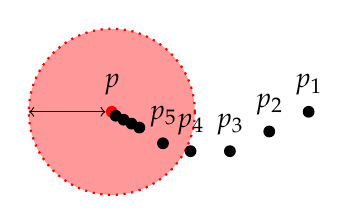
\begin{tikzpicture}[mycirc/.style={circle,fill, minimum size=0.15cm, inner sep = 0pt}]
        \draw[red, dotted, thick, fill = white!60!red] (-1, 0) circle (30pt);
        \node[mycirc, label=above:{$p$}, fill = red] at (-1, 0) {};
        \node[mycirc, label=above:{$p_1$}] at (1.5, 0) {};
        \node[mycirc, label=above:{$p_2$}] at (1, -0.25) {};
        \node[mycirc, label=above:{$p_3$}] at (0.5, -0.5) {};
        \node[mycirc, label=above:{$p_4$}] at (0, -0.5) {};
        \node[mycirc, label=above:{$p_5$}] at (-0.35, -0.4) {};
        \node[mycirc] at (-0.65, -0.2) {};
        \node[mycirc] at (-0.75, -0.15) {};
        \node[mycirc] at (-0.85, -0.1) {};
        \node[mycirc] at (-0.95, -0.05) {};
        \draw[<->] (-1.08, 0) -- (-2.05, 0);
        \node[label=above:{$\e$}] at (-1.5, -0.15) {};
    \end{tikzpicture}
    \caption{Visualization of a sequence $\set{p_n} \subset \RR^2$ converging to a point $p$. For the $\e > 0$ shown in the picture, we have that all points of the sequence past $N = 5$ lie in the open disk of radius $\e$ around $p$.}
    \label{fig15}
\end{figure}

\noindent As a remark, consider that convergence can depend on our choice of metric space; for example, $\set{\frac{1}{n}}$ as a sequence in $\RR$ converges to $0$, but the same sequence in the strictly positive reals ($\RR^+ = \set{x \in \RR: x > 0}$) does not converge.

Another interesting example (that again shows us the importance of the choice of metric space). Is $\RR$ equipped with the discrete metric. A question we can ask is ``given some points $p \in \RR$, what sequences converge to $p$?'' The answer turns out to be eventually constant sequences only; that is, sequences for which $p_n = p$ for $n \geq N$ for some $N$. 
\begin{proof}
    If $p_n \rightarrow p$, then setting $\e = \frac{1}{2}$, we have that there exists $N \in NN$ such that for all $n \geq N$, $d(p_n, p) < \e = \frac{1}{2}$. Under the discrete metric, this is only possible if $p_n = p$. 
\end{proof}
This of course is a strikingly different picture for $\RR$ with the standard metric of $d(x, y) = \abs{x - y}$. For example, the sequnce $p_n = \frac{1}{n}$ has no term equal to zero, but converges to $p = 0$. The takeaway message here can be that in the Euclidean metric, points can ``get closer'' but in the discrete metric, they cannot.

\stepcounter{rudin}
\begin{theorem}{}{3.3}
    Suppose $\set{s_n}, \set{t_n}$ are complex sequences that converge, with $\linf s_n \rightarrow s$ and $\linf t_n \rightarrow t$. Then:
    \begin{enumerate}
        \item $\linf(s_n + t_n) = s + t$.
        \item $\linf cs_n = cs$ and $\linf (c + s_n) = c + s$ for all $c \in \CC$.
        \item $\linf s_nt_n = st$
        \item $\linf \frac{1}{s_n} = \frac{1}{s}$ provided $s \neq 0$ and $s_n \neq 0$ for all $n$.
    \end{enumerate}
\end{theorem}
\begin{nproof}
    \begin{enumerate}
        \item Let $\e > 0$. There exist $N_1, N_2 \in \NN$ such that $\abs{s_{n_1} - s} < \frac{\e}{2}$ for $n_1 \geq N_1$ and $\abs{t_{n_2} - t} < \frac{\e}{2}$ for $n_2 \geq N_2$. Take $N = \max{N_1, N_2}$, and using the triangle inequality, it follows that for $n \geq N$:
        \begin{align*}
            \abs{(s_n + t_n) - (s + t)} \leq \abs{s_n - s} + \abs{t_n - t} < \frac{\e}{2} + \frac{\e}{2} = \e
        \end{align*} 
        We conclude that $\linf (s_n + t_n) = s + t$. 
        \item Let $\e > 0$. If $c = 0$ then the first sequence trivially converges to $0$, so suppose that $c \neq 0$. There exists $N$ such that $\abs{s_n - s} < \frac{\e}{\abs{c}}$ for $n \geq N$, so it follows that:
        \begin{align*}
            \abs{cs_n - cs} = \abs{c}\abs{s_n - s} < \abs{c}\frac{\e}{\abs{c}} = \e.
        \end{align*} For the second identity, we have that $c_n \rightarrow c$ for any constant sequence $c_n = c$ so we may apply (a).
        \item Let $\e > 0$. There exist $N_1, N_2$ such that $\abs{s_{n_1} - s} < \sqrt{2}$ for $n_1 \geq N_1$ and $\abs{t_{n_2} - t} < \sqrt{2}$ for $n_2 \geq N_2$. We then consider that:
        \begin{align*}
        s_nt_n - st = (s_n - s)(t_n - t) + s(t_n - t) + t(s_n - s)
        \end{align*}
        For $n \geq N = \max{N_1, N_2}$, we have that:
        \begin{align*}
            (s_n - s)(t_n - t) < \e
        \end{align*}
        And we hence observe that $\linf (s_n - s)(t_n - t) = 0$. We can then use (a) and (b) to find that:
        \begin{align*}
            \linf s(t_n - t) = 0, \quad \linf t(s_n - s) = 0
        \end{align*}
        So we conclude that $\linf (s_nt_n - st) = 0$ and hence $s_nt_n \rightarrow st$.
    \end{enumerate}
\end{nproof}
\begin{nproofcont}
    \begin{enumerate}
        \setcounter{enumi}{3}
        \item Choose $m$ such that $\abs{s_n - s} < \frac{1}{2}\abs{s}$ if $n \geq m$. We then have that $\abs{s_n} > \frac{1}{2}\abs{s}$ for $n \geq m$. Let $\e > )0$. Then, there exists $N$ with $N > m$ such that for $n \geq N$:
        \begin{align*}
            \abs{s_n - s} < \frac{1}{2}\abs{s}^2\e
        \end{align*}
        Hence, for $n \geq N$:
        \begin{align*}
            \abs{\frac{1}{s_n} - \frac{1}{s}} = \abs{\frac{s_n - s}{s_ns}} < \frac{2}{\abs{s}^2}\abs{s_n - s} < \e
        \end{align*}
        \qed
    \end{enumerate}
\end{nproofcont}

\begin{nlemma}{: Squeeze Lemma}{}
    Let $\set{x_n}$, $\set{s_n}$ be real-valued sequences. Then, if $0 \leq x_n \leq s_n$ for all $n$, and $\linf s_n = 0$, then $\linf x_n = 0$.
\end{nlemma}
\begin{nproof}
    Let $\e > 0$. Choose $N \in \NN$ such that $n \geq N$ implies $0 \leq s_n < \e$. Then, we have that for $n \geq N$, $0 \leq x_n \leq s_n < \e$ and hence $x_n \rightarrow 0$ as claimed. \qed
\end{nproof}

\noindent Note that we can prove a more generalized version of the Squeeze Lemma. 

\begin{nlemma}{: Generalized Squeeze Lemma}{}
    Suppose we have sequences $\set{l_n}, \set{x_n}, \set{u_n}$ such that $l_n \leq x_n \leq u_n$ for all $n$ and $\linf l_n = \linf u_n = L \in \RR$. Then, $\linf x_n = L$.
\end{nlemma}

\begin{nproof}
    We have that $0 \leq a_n - l_n \leq u_n - l_n$. We have that $\linf u_n - l_n = 0$ by Theorem \ref{thm:3.3}(a), so by the (original) Squeeze Lemma we have that $\linf a_n - l_n = 0$. It then follows that $\linf a_n = \linf l_n = L$ as claimed. \qed
\end{nproof}

\setcounter{rudin}{19}
\begin{theorem}{}{3.20}
    \begin{enumerate}
        \item Let $p > 0$. Then, $\linf \frac{1}{n^p} = 0$.
        \item Let $p > 0$. Then, $\linf \sqrt[n]{p} = 1$.
        \item $\linf \sqrt[n]{n} = 1$.
        \item Let $p > 0$ and $\alpha \in \RR$. Then, $\linf \frac{n^\alpha}{(1+p)^n} = 0$.
        \item Let $\abs{x} < 1$. Then, $\linf x^n = 0$. 
    \end{enumerate}
\end{theorem}
\begin{nproof}
    \begin{enumerate}
        \item Let $\e > 0$. Choose $N$ such that $\frac{1}{N^p} < \e$, namely $N > \left(\frac{1}{\e}\right)^{1/p}$. Then, for $n \geq N$, $\frac{1}{n^p} < \frac{1}{N^p} < \e$. 
        
        \item If $p = 1$, the sequence is constant and the conclusion immediate. 
        
        If $p > 1$, then let $x_n = \sqrt[n]{p} - 1$. We then have that:
        \begin{align*}
            p = (x_n + 1)^n = \sum_{k=0}^n \binom{n}{k}x_n^k \geq nx_n
        \end{align*}
        Where the second equality follows from the binomial theorem (where $\binom{n}{k} = \frac{n!}{k!(n-k)!}$), and the inequality follows by considering that we just keep the $k = 1$ term (and the series is non-negative). Hence, we have that $x_n \leq \frac{p}{n}$, and $x_n \rightarrow 0$ by (a). 
        
        If $p < 1$, then let $q = \frac{1}{p} > 1$. Then, $\sqrt[n]{q} \rightarrow 1$ by the argument above. By Theorem \ref{thm:3.3}(d), we then have that $\sqrt[n]{p} = \frac{1}{\sqrt[n]{q}} \rightarrow \frac{1}{1} = 1$.

        \item Let $x_n = \sqrt[n]{n} - 1$. Then, we have that:
        \begin{align*}
            n = (x_n + 1)^n = \sum_{k=0}^n\binom{n}{k}x_n^k \geq \frac{n(n-1)}{2}x_n^2
        \end{align*}
        Where the inequality follows from keeping the $k = 2$ term only. We then have that $x_n \leq \sqrt{\frac{2}{n-1}}$ and hence $x_n \rightarrow 0$ by the Squeeze Lemma.
        \item We want to show $\frac{n^\alpha}{(1+p)^n} \rightarrow 0$; we therefore want an upper bound on the expression, and hence a lower bound on $(1+p)^n$. Applying the Binomial Theorem we have that:
        \begin{align*}
            (1+p)^n = \sum_{k=0}^n\binom{n}{k}p^k = \left((n)(n-1)(n-2)\cdots(n-k+1)\right)\frac{p^k}{n!}
        \end{align*}
        Now, we pick $k > \alpha$. For $2n > k$, we then have that:
        \begin{align*}
            (1+p)^n \geq \left(\frac{n}{2}\right)^k\frac{p^k}{k!}
        \end{align*}
        We therefore have that:
        \begin{align*}
            \frac{n^\alpha}{(1+p)^k} \leq \frac{2^kk!}{p^k}n^{\alpha - k} \rightarrow 0
        \end{align*}
        And the claim follows by the Squeeze Lemma.
        
        \item Taking $\alpha = 0$ in (d), the claim follows by setting $\abs{x} = \frac{1}{1+p} < 1$ (as $p > 0$) and recognizing that $x_n \rightarrow 0 \iff \abs{x^n} = \abs{x}^n \rightarrow 0$. \qed
    \end{enumerate}
\end{nproof}

\subsection{Subsequences}

\setcounter{rudin}{1}
\begin{theorem}{}{3.2}
    Let $\set{p_n}$ be a sequence in $X$.
    \begin{enumerate}
        \item $p_n \rightarrow p$ in $X$ if and only if for all $r > 0$, $N_r(p)$ contains all but finitely many points of $\set{p_n}$.
        \item If $p_n \rightarrow p$ and $p_n \rightarrow p'$ then $p = p'$. In other words, the limit is unique.
        \item If $\set{p_n}$ is convergent, then it is bounded (that is, for any $q \in X$ there exists $M \in \RR$ such that $d(q, p_n) \leq M$ for all $n \in \NN$).
        \item If $E \subset X$ has a limit point $p$, then there exists $\set{p_n}$ in $E$ such that $p_n \rightarrow p$. 
    \end{enumerate}
\end{theorem}
\begin{nproof}
    \begin{enumerate}
        \item The claim follows immediately from the definition of convergence; for any $r = \e > 0$, there exists $N \in \NN$ such that $N_r(p)$ contains $\set{p_n: n \geq N}$.
        \item There exist $N_1, N_2$ such that $d(p, p_{n_1}) < \frac{\e}{2}$ if $n_1 \geq N_1$ and $d(p, p_{n_2}) < \frac{\e}{2}$ if $n_2 \geq N_2$. Then for $n \geq N = \max{N_1, N_2}$ we have (using the triangle inequality) that:
        \begin{align*}
            d(p, p') \leq d(p, p_n) + d(p_n, p') < \frac{\e}{2} + \frac{\e}{2} = \e
        \end{align*}
        Since $\e$ is arbitrary, $d(p, p') = 0$ and hence $p = p'$.

        \item If $p_n \rightarrow p$, there exists $N$ such that $d(p_n, p) < 1$ for all $n \geq N$. Set:
        \begin{align*}
            r = \max\set{1, d(p_1, p), d(p_2, p), \ldots ,d(p_{N-1}, p)}
        \end{align*}
        For any $q \in X$, we then have that:
        \begin{align*}
            d(q, p_n) \leq d(q, p) + d(p, p_n) \leq d(q, p) + r
        \end{align*}
        so the claim follows with $M = r + d(q, p) + 1$.
        \item Pick $p_n \in E$ such that $d(p_n, p) < \frac{1}{n}$. Let $\e > 0$, and $N > \frac{1}{\e}$. Then, $n \geq N$ implies $\frac{1}{n} \leq \frac{1}{N} < \e$ and hence $d(p_n, p) < \e$ for all $n \geq N$, and hence $p_n \rightarrow p$ as desired. \qed
    \end{enumerate}
\end{nproof}

\setcounter{rudin}{4}
\begin{definition}{Subsequences}{3.5}
    Given $\set{p_n}$ and $n_1 < n_2 < n_3 < \ldots$, we say that $\set{p_{n_j}}$ is a \textbf{subsequence} of $\set{p_n}$.
\end{definition}

\noindent We first consider some examples. Let $p_n = n$. Then some valid subsequences of $\set{p_n}$ are $\set{1, 2, 3, 4, 5, \ldots}$ (the original sequence), $\set{1, 3, 5, 7, \ldots}$ (the odds), $\set{2, 3, 5, 7, 11, 13, \ldots}$ (the primes). Next, let $p_n = i^n$. We have that $\set{p_n} = \set{i, -1, -i, 1, i, -1, -i, 1, \ldots}$ which is clearly divergent. However, the subsequences $\set{i, i, i, \ldots}$, $\set{-1, -1, -1, \ldots}$, $\set{-i, -i, -i, \ldots}$ and $\set{1, 1, 1, \ldots}$ are all convergent! It is hence possible for a divergent sequence to have a convergent subsequence.

\begin{nlemma}{}{}
    If $p_n \rightarrow p$, then every subsequence of $\set{p_n}$ converges to $p$. 
\end{nlemma}

\begin{nproof}
    Suppose $p_n \rightarrow p$ and let $\set{p_{n_j}}$ be a subsequence of $p_n$. Let $\e > 0$. Then, there exists some $N \in \NN$ such that $d(p, p_n) < \e$ if $n \geq N$. Hence, $d(p, p_{n_j}) < \e$ if $n_j \geq N$ and hence $p_{n_j} \rightarrow p$. \qed
\end{nproof}

\begin{theorem}{Bolzano–Weierstrass}{3.6}
    \begin{enumerate}
        \item If $\set{p_n} \subset X$ with $X$ compact, then $\set{p_n}$ has a convergenct subsequence.
        \item If $\set{p_n} \subset \RR^k$ and $\set{p_n}$ is bounded, then $\set{p_n}$ has a convergent subsequence.
    \end{enumerate}
\end{theorem}
\begin{nproof}
    \begin{enumerate}
        \item Let $E$ be the range of $\set{p_n}$. If $E$ is finite, then there exists $x \in X$ and $n_1 < n_2 < n_3 < \ldots$ such that $p_{n_j} = x$ for all $j$. Therefore $p_{n_j} \rightarrow x$ and we are done. If $E$ is infinite, then by compactness, $E \subset X$ has a limit point in $X$ by Theorem \ref{thm:2.37}. By Theorem \ref{thm:3.2}(d) there exists a sequence $\set{p_{n_j}}$ in $E$ such that $p_{n_j} \rightarrow p$.
        \item By Theorem \ref{thm:2.41}, $E$ (being bounded) lies in a compact subset of $\RR^k$. We then apply (a). \qed
    \end{enumerate}
\end{nproof}

\subsection{Cauchy Sequences and Completeness}

\setcounter{rudin}{7}
\begin{definition}{Cauchy Sequences}{3.8}
    A sequence $\set{p_n} \subset X$ is a \textbf{Cauchy sequence} if for all $\e > 0$, there exists $N \in \NN$ such that for all $n, m \geq N$, $d(p_n, p_m) < \e$. 
\end{definition}
\noindent Note the fact that this definition does not refer to a particular $p$ that the sequence may converge to! It instead formalizes the notion of the points of a sequence getting ``closer together'' as the sequence goes on. It is therefore easier to check if a sequence is Cauchy than if it converges, as we don't need to know the value of the limit. To this end, it is useful to know in what situations a sequence being Cauchy implies that the sequence is convergent. We will soon arrive at a theorem that addresses this question, but first we establish a little more machinery.

\begin{definition}{Diameter}{3.9}
    Let $E \subset X$. Then the \textbf{diameter} of $E$, denoted $\diam E$ is defined as $\diam E = \sup\set{d(p, q): p, q \in E}$. It follows from the definition that a sequence $\set{p_n}$ is Cauchy if and only if $\lim_{N \rightarrow \infty} \diam E_n = 0$ where $E_n = \set{p_n}_{n=N}^\infty$ (the tail of the sequence).
\end{definition}

\begin{nexample}{}{}
    \begin{enumerate}
        \item If $E = (a, b) \subset \RR$ or $E = [a, b] \subset \RR$, then $\diam E = b - a$.
        \item If $E = (0, 1) \times (0,1) \subset \RR^2$, then $\diam E = \sqrt{2}$ (the diagonal of the open square).
    \end{enumerate}
\end{nexample}

\begin{theorem}{}{3.10}
    \begin{enumerate}
        \item Let $E \subset X$. Then, $\diam \overline{E} = \diam E$.
        \item If $K_n \subset X$ are compact, $K_{n+1} \subset K_n$ for all $n$, and $\linf \diam K_n  = 0$, then $\bigcap_{n=1}^\infty K_n$ consists of exactly one point.
    \end{enumerate}
\end{theorem}

\begin{nproof}
    \begin{enumerate}
        \item Since $E \subset \overline{E}$, it is clear that $\diam \overline{E} \geq \diam E$. Next, let $\e > 0$ and $p, q \in \overline{E}$. Choose $p', q' \in E$ such that $d(p, p') < \frac{\e}{2}$, $d(q, q') < \frac{\e}{2}$ (this choice is possible as either $p, q$ are in $E$, or $p, q$ are limit points of $E$). Then, we have that:
        \begin{align*}
            d(p, q) \leq d(p, p') + d(p', q) \leq d(p, p') + d(p', q') + d(q', q) < \frac{\e}{2} + \diam E + \frac{\e}{2} = \diam E + \e
        \end{align*}
        $\e, p$, and $q$ are arbitrary, so it follows that $\diam \overline{E} \leq \diam E + \e$ from the definition of the diameter. It then follows that $\diam \overline{E} \leq \diam E$. We conclude that $\diam \overline{E} = \diam E$.
        \item Let $K = \bigcap_{n=1}^\infty K_n$. By the corollary to Theorem \ref{thm:2.36}, we have that $K \neq \emptyset$, so $K$ contains at least one point. Since $K \subset K_n$, it follows that $\diam K \leq \diam K_n$ for any $n$, and since $\diam K_n \rightarrow 0$, $\diam K = 0$. If there were $p, q \in K$ such that $p \neq q$, then $\diam K \neq 0$, so it must follow that $K$ has at most one point. We conclude that $K$ has exactly one point. \qed
    \end{enumerate}
\end{nproof}

\begin{nlemma}{}{}
    If a sequence $\set{p_n}$ is Cauchy, then it is bounded.
\end{nlemma}
\begin{nproof}
    If $\set{p_n}$ is Cauchy, then we have that $\lim_{N \rightarrow \infty} \diam E_N = \lim_{N \rightarrow \infty} \diam \set{p_n}_{n = N}^\infty = 0$. Then for some $N \in \NN$, $\diam E_N < 1$. The range of $\set{p_n}$ is the union of $E_N$ and the finite set $\set{p_1, \ldots, p_{N-1}}$ and hence $\set{p_n}$ is bounded. \qed
\end{nproof}

\begin{theorem}{}{3.11}
    \begin{enumerate}
        \item If a sequence $\set{p_n} \subset X$ converges, then it is Cauchy.
        \item If a sequence $\set{p_n} \subset X$ is Cauchy and $X$ is compact, then $\set{p_n}$ converges to some $p \in X$.
        \item In $\RR^k$, every Cauchy sequence is convergent.
    \end{enumerate}
\end{theorem}

\begin{nproof}
    \begin{enumerate}
        \item Let $p_n \rightarrow p$ and let $\e > 0$. There exists $N \in \NN$ such that $d(p_n, p) < \frac{\e}{2}$ if $n \geq N$. Then, for $n, m \geq N$, we have that:
        \begin{align*}
            d(p_n, p_m) \leq d(p_n, p) + d(p, p_m) < \frac{\e}{2} + \frac{\e}{2} = \e
        \end{align*}
        so $\set{p_n}$ is Cauchy.
        \item Let $E_N = \set{p_n}_{n = N}^{\infty}$. Then, $\overline{E}_N \subset X$ is closed, so by the compactness of $X$ we have that $\overline{E}_N$ is compact by Theorem \ref{thm:2.35}. Since $E_{N+1} \subset E_N$, we have that $\overline{E}_{N+1} \subset \overline{E}_N$, and additionally we have that $\lim_{N \rightarrow \infty} \overline{E}_N =\lim_{N \rightarrow \infty} E_N = 0$ where the first equality follows from Theorem \ref{thm:3.10}(a) and the second equality follows from the fact that $\set{p_n}$ is Cauchy and Definition \ref{def:3.9}. Thus, Theorem \ref{thm:3.10}(b) says that there exists a unique point $p \in \bigcap_{n=1}^\infty \overline{E}_N$. Next, let $\e > 0$. Then, there exists $N_0$ such that $\diam \overline{E}_N < \e$ for all $N \geq N_0$. So, $d(p, q) < \e$ for all $q \in \overline{E}_N$, so the same holds for all $q \in E_N$. Hence, $d(p, p_n) < \e$ for all $n \geq N_0$, which shows that $p_n \rightarrow p$ and proves the claim. 
        \item By the above Lemma, Cauchy sequences are bounded. Hence, $\set{p_n} \subset I$ for some $k$-cell $I \subset \RR^k$. Since $I$ is compact in $\RR^k$, the claim follows from (b). \qed
    \end{enumerate}
\end{nproof}

\begin{definition}{Completeness}{3.12}
    A metric space $X$ is called \textbf{complete} if every Cauchy sequence converges in $X$. 
\end{definition}
It might be tempting at first to think that every space would be complete, but this is not the case. For example, something that can go wrong is a sequnece can be Cauchy, but the limit can lie ``outside'' of the space. To see this, consider again the sequence $\set{\frac{1}{n}}$ in the metric space $\RR^+ = \RR \setminus \set{x \in \RR: x \leq 0}$. The sequence is Cauchy, but does not converge in $\RR^+$ (as it converges to 0, which lies outside of the space).

\begin{nexample}{}{}
    \begin{enumerate}[(i)]
        \item Compact sets are complete by Theorem \ref{thm:3.11}(b).
        \item $\RR^k$ (and $\CC$) are complete by Theorem \ref{thm:3.11}(c).
        \item $\QQ$ is not complete. We can make a sequence of rational points that converges to an irrational number in $\RR$ which is Cauchy, but does not converge in $\QQ$ (Example \ref{exam:1.1b} gives a way one might construct such a sequence). 
    \end{enumerate}
\end{nexample}
\noindent Note that $\QQ$ can be completed to $\RR$, and in general for any $(X, d)$ which is not complete, there exists $(X^*, d^*)$ that is complete such that $\abs{X} = X^*$. Indeed, this is another way we can construct the real numbers! $\RR$ can be viewed as equivalence classes of Cauchy sequences in $\QQ$. The idea is to define an equivalnence relation $\sim$ such that $p_n \sim q_n$ if $\linf d(p_n, q_n) = 0$. $X^*$ is then defined as the set of equivalence classes under that equivalence relation, equipped with the metric $d^*([p], [q]) = \linf d(p_n, q_n)$. It can then be checked that $d^*$ is a valid metric and that $X^*$ is complete. For the full proof, see HW7, or exercises 3.23-3.25 in Rudin (note: this proof is quite technical/difficult).

To motivate the next theorem, consider that all convergent sequences in $\RR$ (and in general) are bounded (as we saw in Theorem \ref{thm:3.2}(c)). However, this is not always true; for example consider $p_n = (-1)^n$ which is clearly bounded but divergent. What then are conditions that a bounded sequence may converge?

\begin{definition}{Monotonic Sequences}{3.13}
    A sequence $\set{p_n} \subset \RR$ is \textbf{monotonically increasing} if $p_{n+1} \geq p_n$ for all $n$, and \textbf{montonically decreasing} if $p_{n+1} \leq p_n$.
\end{definition}

\begin{theorem}{}{3.14}
    Suppose $\set{p_n} \subset \RR$ is montonic. Then, $\set{p_n}$ is convergent if and only if it is bounded. 
\end{theorem}

\begin{nproof}
    $\boxed{\implies}$ See Theorem \ref{thm:3.2}(c).

    $\boxed{\impliedby}$ We show the proof for the increasing case as the decreasing case is analogous. Let $p = \sup{p_n: n \in \NN}$ which exists as $\set{p_n}$ is bounded and $\RR$ has the LUB property. Then, $p_n \leq p$ for all $n$. Let $\e > 0$. Then, there exists $N \in \NN$ such that $p - \e < p_{N} < p_{N+1}$. By the monotonicity of $\set{p_n}$, it follows that $\abs{p_n - p} < \e$ for all $n \geq N$. Hence, $p_n \rightarrow p$. \qed
\end{nproof}

\begin{definition}{Limits to Infinity}{3.15}
    Let $\set{p_n} \subset \RR$. If for all $M \in \RR$, there exists $N \in \NN$ such that $p_n > M$ for all $n \geq N$, then we write $p_n \rightarrow \infty$. If instead for all $M \in \RR$ there exists $N \in \NN$ such that $p_n < M$ for all $n \geq N$, then we write $p_n \rightarrow -\infty$.
\end{definition}



\subsection{Limit Supremum and Limit Infimum}
As a motivating question, how would we say something about the largest and smallest accumulation points of a sequence? This leads us to the following definition.
\begin{definition}{limsup and liminf}{3.16}
    Let $\set{s_n} \subset \RR$, then, we define the \textbf{limit supremum} as:
    \begin{align*}
        \limsup_{n \rightarrow \infty} s_n = \inf_{n \geq 1}\sup_{m \geq n} s_m = \lim_{n \rightarrow \infty} \sup_{m \geq n} s_m
    \end{align*}
    And the \textbf{limit infimum} as:
    \begin{align*}
        \liminf_{n \rightarrow \infty} s_n = \sup_{n \geq 1}\inf_{m \geq n} s_m = \lim_{n \rightarrow \infty} \inf_{m \geq n} s_m
    \end{align*}
    Note that unlike the limit of a real-valued sequence, the limsup and liminf always exist.
\end{definition}

\noindent In the above definition, the equivalence of $inf_{n \geq 1}\sup_{m \geq n} s_m$ and $\lim_{n \rightarrow \infty} \sup_{m \geq n} s_m$ may be slightly confusing. To see this, consider the fact that the sequence $q_n = \sup \set{p_n: n \geq 1}$ is a strictly decreasing sequence in $n$ (with increasing $n$, we take the supremum over less terms each time), so taking the limit of $n \rightarrow \infty$ or taking the infimum over $n$ are equivalent. 

Note that Rudin defines the limsup/liminf differently, but perfectly equivalently. Namely, if $\set{p_n} \subset \RR$ is a sequence, then $E$ is the set of all subsequential limits (i.e. there is a subsequence of $\set{p_n}$ with a given limit). Then, $\limsup^* p_n = \sup E$ (we use the $*$ to denote Rudin's definition). The equivalence is not immediately obvious, so we here give a sketch to show that the two definitions coincide. We will use the general technique of showing that the two expressions are $\e$ close to one another. Namely, for any $\e > 0$, we show that the following two statements hold:
\begin{enumerate}[1)]
    \item $\limsup^* p_n \leq \limsup p_n + \e$
    \item $\limsup^* p_n + \e \geq \limsup p_n$
\end{enumerate}
To show 1), for each $N$, we let $n_N$ be an index such that $p_{n_N}$ satisfies:
\begin{align*}
    p_{n_N} \geq \sup\set{p_n: n \geq N} - \frac{\e}{N}
\end{align*}
And then we claim that $\linf p_{n_N} = \limsup p_n$ (Exercise). There is one slight technical issue in that $\set{p_{n_N}}$ may not be a subsequence of $\set{p_n}$, in particular we don't know that $n_{N_1} < n_{N_2} < n_{N_3} < \ldots$ just by the above construction (but in order for this to be a valid subsequence, we need this to be the case). Fortunately, this is a fixable issue. We do know that $n_{N_1} \geq 1$, $n_{N_2} \geq 2$, $n_{N_3} \geq 3$ by construction, so if it turns out to be the case that $n_{N_1} < n_{N_2}$ doesn't hold, we can skip ahead into the sequence until we find the first $j$ for which the equality holds. Concretely, if $n_{N_1} = 1000$ (as an example), then if we skip ahead to $n_{N_{1001}}$, it is guaranteed that $n_{N_1} < n_{N_{1001}}$ and we can from there construct a valid sequence. The sketch for 2) is left as an exercise. 

\begin{nexample}{}{}
    \begin{enumerate}
        \item Consider $s_n = (-1)^n\left(1 + \frac{1}{n^2}\right)$. Then, we have that $1 \leq \sup_{m \geq n} s_n \leq 1 + \frac{1}{1^2} = 2$, so $\limsup_{n \rightarrow \infty} s_n = 1$. Similarly, $\limsup_{n \rightarrow \infty} s_n = -1$. Note that this sequence has no limit (it oscillates indefinitely and does not converge) but these quantities are well defined. We notice that the limsup is greater than the liminf in this case, and indeed it is true in general that $\liminf_{n \rightarrow \infty} s_n \leq \limsup_{n \rightarrow \infty} s_n$. 
        \item If $\set{s_n}$ is not bounded above, then $\sup_{m \geq n} s_n = \infty$ for all $n$ and we write $\limsup_{n \rightarrow} s_n = \infty$. Similarly, if $\set{s_n}$ is not bounded below, then $\inf_{m \geq n} s_n = -\infty$ for all $n$ and we write $\limsup_{n \rightarrow \infty} s_n = -\infty$.
    \end{enumerate}
\end{nexample}

\noindent One difficulty with discussing the convergence of a sequence is that the definition is difficult to apply; we need to know what the sequence converges to. The notion of a Cauchy sequence then begins helpful (as Cauchy and convergent are equivalent in complete metric spaces). In addition, it is helpful to consider the limsup and liminf, as we can bound the limit above and below with these quantities respectively. In particular, the limit of the supremum of the tail of the sequence equals the limit of the infinimum of the tail of the sequence equals the limit of the sequence if the sequence is convergent.

\setcounter{rudin}{17}
\begin{theorem}{}{3.18}
    Let $\set{s_n} \subset \RR$. Then, $\linf s_n = L$ if and only if $\limsup_{n \rightarrow \infty} s_n = \liminf_{n \rightarrow \infty} = L$.
\end{theorem}
\begin{nproof}
    $\boxed{\implies}$ Let $\e > 0$. Then, there exists $N \in \NN$ such that $s_m \in (L - \e, L + \e)$ for all $m \geq N$> Then, we have that:
    \begin{align*}
        L - \e \leq \inf_{m \geq N} s_m \leq \sup_{m \geq N} \leq L + \e
    \end{align*}
    Taking limits we have:
    \begin{align*}
        L - \e \leq \liminf_{n \rightarrow \infty} \leq \limsup_{n \rightarrow \infty} s_n  \leq L + \e
    \end{align*}
    $\e$ is arbitrary, so we have that $\limsup_{n \rightarrow \infty} s_n = \liminf_{n \rightarrow \infty} = L$ .

    $\boxed{\impliedby}$ We have that:
    \begin{align*}
        \inf_{m \geq n} s_n \leq s_n \leq \sup_{m \geq n} s_m
    \end{align*}
    for all $n \in \NN$. By assumption we have $\limsup_{n \rightarrow \infty} s_n = \liminf_{n \rightarrow \infty} = L$ so by the Generalized Squeeze Lemma we conclude that $\linf s_n = L$. \qed
\end{nproof}
\subsection{Series}

\setcounter{rudin}{20}
\begin{definition}{Infinite Series}{3.21}
    Let $\set{a_n} \subset \CC$. We then form a new sequence of $s_n = \sum_{j=1}^n a_j$ (the sequence of partial sums). Then, if $s_n \rightarrow s$. We say that the series $\sum_{j = 1}^\infty a_j$ converges, and write $\sum_{j = 1}^\infty a_j = s$. If $s_n$ does not converge, we say that $\sum_{j=1}^\infty a_j$ diverges. As a notational point, we will sometimes omit the bounds of summation and write $\sum a_j$ to denote an infinite series, where the meaning is clear from context.
\end{definition}
\noindent Note that series are just a specific subset of sequences. Although the above definition states that $\set{a_n} \subset \CC$, it is in general possible to define series over general vector spaces, with $\set{a_n} \in V$ and $\set{s_n} \in V$. 

Note that this generalization allows us to state an equivalent notion of completeness for vector spaces, namely that $V$ is compelte if and only if for all sequences $\set{a_n} \subset V$, the sum $\sum_{n=0}^\infty \norm{a_n}$ converges to a point in $V$. As before, $\RR, \RR^k$ (both over the field $\RR$), are complete vector spaces. An example of a vector space that is not complete is the set of functions $f: \RR \mapsto \CC$ such that $\int_{-\infty}^\infty \abs{f(x)}^2 dx < \infty$ (where the integral is the familiar Riemann integral from first year calculus, to be defined more rigorously in Chapter 6). For example, the sequence $f_n \subset V$ such that:
\begin{align*}
    f_n = \begin{cases}
        1 & \text{for the first $n$ rationals}
        \\ 0 & \text{elsewhere}
    \end{cases}
\end{align*}
does not converge to a function in $V$. In fact, Lebesgue integration (which is not covered in this course, but will be the primary focus of a course in measure theory) deals with this issue.

We will now restate the Cauchy criterion (Theorem \ref{thm:3.11}) for series.

\begin{theorem}{}{3.22}
    A series $\sum a_j$ converges if and only if for all $\e > 0$, there exists $N \in \NN$ such that $\abs{\sum_{j=m}^n a_j} < \e$ for all $n \geq m \geq N$.
\end{theorem}
\begin{nproof}
    $\sum a_j$ converges if and only if $\set{s_n}$ converges if and only if $\set{s_n}$ is Cauchy. So by definition there exists $N$ such that for $n \geq m - 1 \geq N$:
    \begin{align*}
        \abs{s_n - s_m} = \abs{\sum_{j=1}^n a_j - \sum_{j=1}^{m-1} a_j} = \abs{\sum_{j=m}^n a_j} < \e
    \end{align*}
    which proves the claim. \qed
\end{nproof}

\begin{theorem}{Divergence Test}{3.23}
    If $\sum a_n$ converges, then $\linf a_n = 0$.
\end{theorem}
\begin{nproof}
    Choose $n = m$ in Theorem \ref{thm:3.22}. \qed
\end{nproof}
\noindent Note that this criteria gives us the ability to easily check if a series diverges; if $a_j$ does not converge to $0$, then $\sum a_j$ diverges. However, note that the reverse implication does NOT hold! $\sum \frac{1}{n}$ diverges (as we will show next lecture) even though clearly $\frac{1}{n} \rightarrow 0$. 

\begin{theorem}{}{3.24}
    Let $\set{a_n} \subset \RR$ and $a_n \geq 0$ for all $n$. Then, we have that $\sum a_n$ converges if and only if the sequence of partial sums $\set{s_n}$ is bounded.
\end{theorem}
\begin{nproof}
    If $a_n \geq 0$, then $\set{s_n}$ is monotonically increasing. Then by Theorem \ref{thm:3.14}, $\set{s_n}$ converges if and only if it is bounded. \qed
\end{nproof}

\begin{theorem}{Comparison Test}{3.25}
    \begin{enumerate}
        \item Let $\set{a_n} \subset \CC$ and $\set{c_n} \subset \RR$. Then, if $\abs{a_n} \leq c_n$ for all $n \geq N_0$ for some $N_0 \in \NN$, and $\sum c_n$ converges, then $\sum a_n$ converges. 
        \item Let $\set{a_n} \subset \RR$ and $\set{d_n} \subset \RR$. If $a_n \geq d_n \geq 0$ for all $n \geq N_0$ for some $N_0 \in \NN$ and $\sum d_n$ diverges, then $\sum a_n$ diverges.
    \end{enumerate}
\end{theorem}
\begin{nproof}
    \begin{enumerate}
        \item Let $\e > 0$. Then, there exists $N \in \NN$ such that $\sum_{j = m}^n c_n < \e$ for all $n \geq m \geq N$. Then, take $N \geq N_0$, and we have that:
        \begin{align*}
            \abs{\sum_{j=m}^n a_j} \leq \sum_{j=m}^n \abs{a_j} \leq \sum_{j=m}^n c_j < \e
        \end{align*}
        Where in the first inequality we apply the triangle inequality (Theorem \ref{thm:1.37}). We conclude that $\sum a_j$ converges by the Cauchy criterion (Theorem \ref{thm:3.22}).
        \item The claim follows by considering the contrapositive of (a). \qed
    \end{enumerate}
\end{nproof}

\begin{theorem}{The Geometric Series}{3.26}
    If $0 \leq x < 1$, then $\sum_{j=0}^\infty x^j = \frac{1}{1-x}$. If $x \geq 1$, then $\sum_{j=0}^\infty x^j$ diverges.
\end{theorem}
\begin{nproof}
    Suppose $x = 1$. Then, $x_n = 1$ does not converge to zero, so by Theorem \ref{thm:3.24} $\sum_{j=0}^\infty x^j$ diverges. Suppose then that $x \neq 1$. We have that $s_n = 1 + x + x^2 + \ldots + x^n$. Hence, $xs_n = x + x^2 + x^3 + \ldots + x^n + x^{n+1}$. Hence, $(1-x)s_n = 1 + x^{n+1}$ and therefore a closed form expression for $s_n$ is:
    \begin{align*}
        s_n = \frac{1 + x^{n+1}}{1 - x}
    \end{align*}
    If $x > 1$, we have that $s_n$ diverges (again) by Theorem \ref{thm:3.24}. If $x < 1$, then $x^{n+1} \rightarrow 0$ by \ref{thm:3.20}(e), so $s_n \rightarrow \frac{1}{1-x}$. \qed
\end{nproof}
\noindent Note that by the comparison test, the above result can be generalized to see that $\sum z^j$ for $z \in \CC$ converges for $\abs{z} < 1$ and diverges for $\abs{z} \geq 1$. 

\begin{theorem}{Cauchy Condensation Test}{3.27}
    Suppose $\set{a_n} \subset \RR$ and $a_1 \geq a_2 \geq a_3 \geq \ldots \geq 0$. Then, $\sum a_j$ converges if and only if $\sum_{n=1}^\infty 2^n a_{2^n}$ converges.
\end{theorem}
\begin{nproof}
    $\boxed{\implies}$ For $2^k < n$, using the fact that the sequence is decreasing, we have that:
    \begin{align*}
        a_1 + a_2 + \ldots + a_n &\geq a_1 + a_2 + (a_3 + a_4) + \ldots + (a_{2^{k-1}+1} + \ldots + a_{2^k})
        \\ &\geq \frac{1}{2}a_1 + a_2 + 2a_4 + \ldots + 2^{k-1}a_{2^k}
        \\ &= \frac{1}{2}(a_1 + 2a_2 + 4a_4 + \ldots + 2^ka_{2^k})
    \end{align*}
    Hence by the comparison test (Theorem \ref{thm:3.25}) we have that $\sum 2^n a_{2^n}$ converges if $\sum a_j$ converges.

    $\boxed{\impliedby}$ We show the contrapositive. For $2^k > n$, We have that:
    \begin{align*}
        a_1 + a_2 + \ldots + a_n &\leq a_1 + (a_2 + a_3) + \ldots + (a_{2^k} + \ldots + a_{2^{k+1}-1})
        \\ &\leq a_1 + 2a_2 + 4a_4 + \ldots + 2^ka_{2^k}
    \end{align*}
    Hence by the comparison test (Theorem \ref{thm:3.25}) we have that $\sum 2^n a_{2^n}$ diverges if $\sum a_j$ diverges. \qed
\end{nproof}

\subsection{p-Series and Euler's Number}
We now use the result of Theorem \ref{thm:3.27} to prove a result about a familiar subset of series.

\begin{theorem}{p-Series}{3.28}
    $\sum_{n=1}^\infty \frac{1}{n^p}$ converges if $p > 1$ and diverges if $p \leq 1$. 
\end{theorem}
\begin{nproof}
    If $p \leq 0$, then $n^p$ does not converge to $0$ and hence $\sum \frac{1}{n^p}$ diverges by Theorem \ref{thm:3.23}. If $p > 0$, then $\frac{1}{n^p}$ is a monotonically decreasing sequence of positive terms. Hence, we can apply the result of Theorem \ref{thm:3.27}. $\sum \frac{1}{n^p}$ converges if and only if $\sum_k 2^k \frac{1}{2^{kp}} = \sum_k \left(\frac{1}{2^{p-1}}\right)^k$ converges. By Theorem \ref{thm:3.26}, this last expression is convergent if and only if $0 < \frac{1}{2^{p-1}} < 1$, i.e. if $p > 1$, proving the claim. \qed
\end{nproof}
\noindent From the above result, we have that the $p$-series converges if $p > 1$ and diverges otherwise. Is there something ``in between'' these two regions?

\begin{theorem}{}{3.29}
    $\sum_{n=2}^\infty \frac{1}{n(\log n)^p}$ converges if $p > 1$ and diverges if $p \leq 1$.
\end{theorem}
\begin{nproof}
    $\log n$ is monotonically increasing for $p > 0$. So, $\frac{1}{n(\log n)^p}$ is monotonically decreasing. Hence, $\sum \frac{1}{n(\log n)^p}$ converges if and only if $\sum_k 2^k \frac{1}{2^k}\frac{1}{(\log 2^k)^p} = \sum_k \frac{1}{k^p}$ converges, and hence the claim follows from Theorem \ref{thm:3.28}. \qed
\end{nproof}

\begin{definition}{Euler's Number}{3.30}
    $e = \sum_{n=0}^\infty \frac{1}{n!}$, where $0! = 1$ and $n! = n\cdot (n-1)! = n \cdot (n-1) \cdot \ldots \cdot 2 \cdot 1$ for $n \geq 1$. 
\end{definition}
\noindent We should check that this expression is well defined (namely, that the series converges). We first observe that $\frac{1}{n!} \leq \frac{1}{2^{n-1}}$ for $n \geq 1$. Therefore, we have that:
\begin{align*}
    s_n = \sum_{j=0}^n \frac{1}{j!} \leq 1 + \sum_{j=1}^n \frac{1}{2^{j-1}} \leq 1 + \sum_{j=0}^\infty \frac{1}{2^j} = 1 + \frac{1}{1-\frac{1}{2}} = 3
\end{align*}
Where we use Theorem \ref{thm:3.26} in the second last equality. Hence, we conclude that $\sum_{j=0}^n \frac{1}{j!}$ converges by comparison, and moreover, that $0 < e < 3$. 

It will also be of interest to investigate the rate of convergence of this series. To this end, we observe:

\begin{align*}
    0 < e - s_q = \frac{1}{(q+1)!} + \frac{1}{(q+2)!} + \ldots &\leq \frac{1}{(q+1)!}\left(1 + \frac{1}{q+1} + \frac{1}{(q+1)^2} + \ldots \right) 
    \\ &= \frac{1}{(q+1)!}\frac{1}{1-\frac{1}{q+1}} = \frac{1}{(q+1)!}\frac{q+1}{q} = \frac{1}{q!q}
\end{align*}
Hence we have that the error goes to zero extremely quickly! Moreover, we can use this fact to show that $e$ is irrational.

\setcounter{rudin}{31}
\begin{theorem}{Irrationality of e}{3.32}
    $e \notin \QQ$.
\end{theorem}
\begin{nproof}
    Suppose $e = \frac{p}{q}$ for $p, q \in \NN$. Then, by the argument above, we have that $0 < e - s_q < \frac{1}{q!q}$. Hence, we have that $0 < q! q - q!s_q < \frac{1}{q} \leq 1$. But, $q!e = q!\frac{p}{q} = (q-1)!p \in \NN$, and $q!s_q = \sum_{j=0}^q q!\frac{1}{j!} \in \NN$. Hence, $q! e - q! s_q \in \ZZ$, but this is a contradiction as $0 < q! e  - q! s_q < 1$. \qed
\end{nproof}
\noindent There is another familiar definition of $e$ involving a limit that one may recall from first year calculus. These definitions are equivalent, as we will show in the next theorem.

\setcounter{rudin}{30}
\begin{theorem}{}{3.31}
    $e = \linf \left(1 + \frac{1}{n}\right)^n$.
\end{theorem}
\begin{nproof}
    Let $t_n = \left(1 + \frac{1}{n}\right)^n$. By the Binomial theorem, we have that:
    \begin{align*}
        t_n = \sum_{j=0}^n \binom{n}{j}\left(\frac{1}{n}\right)^j = \sum_{j=0}^n \frac{1}{j!}\left(\frac{n}{n}\cdot\frac{(n-1)}{n}\cdots \frac{(n-j+1)}{n}\right) \leq s_n
    \end{align*}
    Where the last inequality follows from the fact tha the term in brackets is less than (or equal to) 1. Hence, we have that $\limsup_{n \rightarrow \infty} t_n \leq \limsup_{n\rightarrow \infty} s_n = \linf s_n = e$. 

    On the other hand, fix $m \in \NN$ and let $n \geq m$. Then, we have that:
    \begin{align*}
        t_n \geq \sum_{j=0}^m \binom{n}{j}\frac{1}{n^j} = \sum_{j=0}^m \frac{1}{j!}\left(\left(1 - \frac{1}{n}\right)\left(1 - \frac{2}{n}\right) \cdots \left(1 - \frac{j-1}{n}\right)\right)
    \end{align*}
    The infimum of the term in the brackets is just $1$, so we therefore have that:
    \begin{align*}
        \inf_{n \geq m} t_n = \sum_{j=0}^m \frac{1}{j!} = s_m
    \end{align*}
    Now, we take $m \rightarrow \infty$ to find that $\liminf_{m \rightarrow \infty} t_m \geq \liminf_{m \rightarrow \infty} s_m = \lim_{m \rightarrow \infty} s_m = e$. 

    Having shown that $\liminf_{n \rightarrow \infty} t_n \geq e \geq \limsup_{n \rightarrow \infty} t_n$, we conclude that $\limsup_{n \rightarrow \infty} = \liminf_{n \rightarrow \infty} = e$ and hence $\linf t_n = e$. \qed
\end{nproof}

\subsection{The Ratio and Root Tests}
\setcounter{rudin}{32}
\begin{theorem}{The Root Test}{3.33}
    Let $\sum a_n$ be a series, and put $\alpha = \limsup_{n \rightarrow \infty} \sqrt[n]{\abs{a_n}}$. Then,
    \begin{enumerate}[(i)]
        \item $\sum a_n$ converges if $\alpha < 1$.
        \item $\sum a_n$ diverges if $\alpha > 1$. 
        \item If $\alpha = 1$, the test is inconclusive.
    \end{enumerate}
\end{theorem}

\begin{nproof}
    \begin{enumerate}[(i)]
        \item Suppose $\limsup_{n \rightarrow \infty} \sqrt[n]{\abs{a_n}} = \alpha < 1$. Take $\beta$ such that $\alpha < \beta < 1$ and $N \in \NN$ such that $\sqrt[n]{\abs{a_n}} < \beta$ for all $n \geq N$. Hence, for $n \geq N$, $\abs{a_n} < \beta^n$, and $\beta < 1$. The result follows by using the comparison Test with the geometric series.
        \item Suppose $\limsup_{n \rightarrow \infty} \sqrt[n]{\abs{a_n}} = \alpha > 1$. Then, there exists a subsequence such that $\sqrt[n_j]{\abs{a_{n_j}}} \rightarrow \alpha$. Therefore, there exists $N$ such that for $j \geq N$, $\sqrt[n_j]{\abs{a_{n_j}}} > 1$, that is to say, $\sqrt[n_j]{\abs{a_{n_j}}} > 1$ for infinitely many terms. Hence, $\sqrt[n]{\abs{a_{n}}}$ does not converge to zero, and hence the series does not converge by the divergence test.
        \item Consider $\sum \frac{1}{n}$ and $\sum \frac{1}{n^2}$. $\alpha = 1$ for both sums, but by Theorem \ref{thm:3.28} the former diverges and the latter converges. \qed
    \end{enumerate}
\end{nproof}

\begin{theorem}{The Ratio Test}{3.34}
    Let $\sum a_n$ be a series such that $a_n \neq 0$ for all $n$. Then,
    \begin{enumerate}[(i)]
        \item $\sum a_n$ converges if $\limsup_{n \rightarrow \infty} \abs{\frac{a_{n+1}}{a_n}} < 1$. 
        \item Diverges if there exists $N_0$ such that $\abs{\frac{a_{n+1}}{a_n}} \geq 1$ for all $n \geq N_0$. 
    \end{enumerate}
\end{theorem}
\noindent In other cases, the test is inconclusive.
\begin{nproof}
    \begin{enumerate}[(i)]
        \item By assumption, there exists $\beta < 1$ such that for some $N$, $\abs{\frac{a_{n+1}}{a_n}} < \beta$ for all $n \geq N$. We then have that $\abs{a_{N+1}} < \beta \abs{a_N}$, that $\abs{a_{N+1}} < \beta \abs{a_{N+1}} < \beta^2 \abs{a_N}$ and inductively we obtain that $\abs{a_{N+p}} < \beta^p \abs{a_N}$. In other words, we have that for $n \geq N$, $\abs{a_n} < \abs{a_N}\beta^{-N}\beta^{n}$. Since $\sum \beta^n$ converges (convergent geometric series), $\sum a_n$ converges by the comparison test.
        \item For $n \geq N_0$, we have that $\abs{a_n} \leq \abs{a_{N+1}}$. Hence, $a_n$ does not converge to 0, and the claim follows by the divergence test. \qed
    \end{enumerate}
\end{nproof}
\noindent As a remark, the the ratio test is less powerful than the root test. For any series for which the ratio test is conclusive, the root test is also conclusive. But the converse is not true. However, the ratio test is easier to apply in practice. We also note that the above ratio test implies the (perhaps more familiar) version from first year calculus:
\begin{ncorollary}{}{}
    Let $\sum a_n$ be a series such that $a_n \neq 0$ for all $n$. Then:
    \begin{enumerate}[(i)]
        \item $\sum a_n$ converges if $\linf \abs{\frac{a_{n+1}}{a_n}} < 1$.
        \item $\sum a_n$ diverges if $\linf \abs{\frac{a_{n+1}}{a_n}} > 1$.
        \item $\sum a_n$ diverges if $\liminf \abs{\frac{a_{n+1}}{a_n}} > 1$.
    \end{enumerate}
\end{ncorollary}

\begin{example}{}{3.35}
    Consider the series:
    \begin{align*}
        \frac{1}{2} + 1 + \frac{1}{8} + \frac{1}{4} + \frac{1}{32} + \frac{1}{16} + \ldots
    \end{align*}
    We then have that the ratio $\frac{a_{n+1}}{a_n}$ is the sequence $2, \frac{1}{8}, 2, \frac{1}{8}, \ldots$. Therefore, $\limsup_{n \rightarrow \infty} \abs{\frac{a_{n+1}}{a_n}} = 2 > 1$ and $\liminf_{n \rightarrow \infty} \abs{\frac{a_{n+1}}{a_n}} = \frac{1}{8} < 1$ and the ratio test is inconclusive/tells us nothing. We then consider the root test. For $n \geq 3$, we have that:
    \begin{align*}
        a_n = \begin{cases}
            \left(\frac{1}{4}\right)^k = \left(\frac{1}{4}\right)^{\frac{n-1}{2}} = 2\left(\frac{1}{4}\right)^{\frac{n}{2}} & n = 2k + 1
            \\ \frac{1}{2}\left(\frac{1}{4}\right)^{k} = \frac{1}{2}\left(\frac{1}{4}\right)^{\frac{n}{2}} & n = 2k
        \end{cases}
    \end{align*}
    Since $\linf \sqrt[n]{p} = 1$ for $p > 0$ (Theorem \ref{thm:3.20}(b)), we have that:
    \begin{align*}
        \linf \sqrt[n]{a_n} = \linf \sqrt[n]{c\left(\frac{1}{4}\right)^{\frac{n}{2}}} = \linf \sqrt[n]{c} \frac{1}{2} = \frac{1}{2} < 1
    \end{align*}
    where the above limit holds for either $c = \frac{1}{2}$ or $c = 2$. Hence, we conclude that the series converges by the root test. This example demonstrates how the root test is ``sharper'' than the ratio test (though harder to apply).
\end{example}

\subsection{Power Series}

\setcounter{rudin}{37}
\begin{definition}{Power Series}{3.38}
    For $z \in \CC$ and a sequence $\set{c_n}$, $\sum_{n=0}^\infty c_n z^n$ is called a \textbf{power series}.
\end{definition}

\begin{theorem}{Radius of Convergence}{3.39}
    Let $R = \frac{1}{\limsup_{n \rightarrow \infty}\sqrt[n]{\abs{c_n}}}$, with the convention $R = \infty$ if $\limsup_{n \rightarrow \infty}\sqrt[n]{\abs{c_n}} = 0$ and $R = 0$ if $\limsup_{n \rightarrow \infty}\sqrt[n]{\abs{c_n}} = \infty$. Then, $\sum_{n=0}^\infty c_n z^n$ converges if $\abs{z} < R$ and diverges if $\abs{z} > R$. $R$ is called the \textbf{radius of convergence} of $\sum c_n z_n$. We note that on the circle $\abs{z} = R$, the behavior is varied; the series can be divergent or convergent, and it can also depend on the particular choice of $z$ on the circle.
\end{theorem}

\begin{nproof}
    We have that $\limsup_{n \rightarrow \infty} \sqrt[n]{c_n z^n} = \limsup_{n \rightarrow \infty} \sqrt[n]{c_n} \abs{z} = \frac{\abs{z}}{R}$. Therefore, by the root test (Theorem \ref{thm:3.33}) the series converges if $\abs{z} < R$ and diverges if $\abs{z} > R$ (and nothing can be said if $\abs{z} = R$). \qed
\end{nproof}
\noindent Note that we can use the ratio test to determine $R$ as well, as we will see in the next few examples.

\begin{example}{}{3.40}
    \begin{enumerate}
        \item $\sum n! z^n$. By the ratio test, we have that $\linf \abs{\frac{(n+1)!z^{n+1}}{n!z^n}} = \linf (n+1)\abs{z} = \infty$ for all $z \neq 0$. Hence the diverges for all $z \in \CC \neq \set{0}$, and we conclude that $R = 0$. 
        \item $\sum \frac{z^n}{n^n}$. By Theorem \ref{thm:3.39}, we have that:
        \begin{align*}
            R = \frac{1}{\limsup_{n \rightarrow \infty}\sqrt[n]{\frac{1}{n^n}}} = \frac{1}{\limsup_{n \rightarrow \infty} \frac{1}{n}} = \frac{1}{\linf \frac{1}{n}} = \infty
        \end{align*}
        \item $\sum \frac{z^n}{n!}$ also has $R = \infty$ (as can be checked easily with the ratio test). For $R = 1$, the series is equal to $e$. As we will define later in Chapter 8, this series is equal to $e^z$. 
        \item $\sum \frac{z^n}{n^p}$ with $p > 1$. By Theorem \ref{thm:3.39}, we have that:
        \begin{align*}
            R = \frac{1}{\limsup_{n \rightarrow \infty}\sqrt[n]{\frac{1}{n^p}}} = \frac{1}{\limsup_{n \rightarrow \infty} \left(\frac{1}{\sqrt[n]{n}}\right)^p} = \frac{1}{1^p} = 1
        \end{align*}
        where for the second last equality we apply Theorem \ref{thm:3.20}(c). Note that this series converges for all $\abs{z} \leq 1$ (although the above calculation does not show convergence on the boundary).
    \end{enumerate}
\end{example}
\noindent Before moving on, let us consider some further examples. Suppose $a_n = 1$ for all $n$. Then, our power series if just $\sum_{n=0}^\infty z^n$, which is just the Geometric series. By Theorem \ref{thm:3.26}, we have that the series converges if $\abs{z} < 1$ to $\frac{1}{1-z}$.
\begin{figure}[htbp]
    \centering
    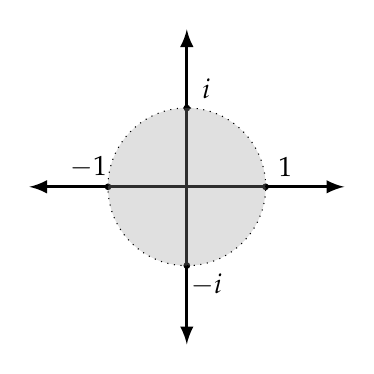
\begin{tikzpicture}
        \draw[latex-latex,very thick] (-2,0)--(2,0);
        \draw[latex-latex,very thick] (0,-2)--(0,2);
        \draw[fill = black] (0, 1) circle (1pt);
        \node[xshift = 0.25cm, yshift = 0.25cm] at (0, 1) {$i$};
        \draw[fill = black] (1, 0) circle (1pt);
        \node[xshift = 0.25cm, yshift = 0.25cm] at (1, 0) {$1$};
        \draw[fill = black] (-1, 0) circle (1pt);
        \node[xshift = -0.25cm, yshift = 0.25cm] at (-1, 0) {$-1$};
        \draw[fill = black] (0, -1) circle (1pt);
        \node[xshift = 0.25cm, yshift = -0.25cm] at (0, -1) {$-i$};
        \draw[dotted, fill = white!60!black, fill opacity=0.3] (0, 0) circle (28.5pt);
        \node[] at (1.6, 1.6) {$\CC$};
    \end{tikzpicture}
    \caption{Visualization of the radius of convergence of the Geometric Series. The series converges in the shaded region, and diverges outside of it (and on the boundary).}
    \label{fig16}
\end{figure}


As another example, consider the series $\sum_{n=1}^\infty \frac{1}{n}z^n$. By the ratio test, we find that $R = 1$, as:
\begin{align*}
    \limsup_{n\rightarrow \infty} \abs{\frac{\frac{1}{n+1}z^{n+1}}{\frac{1}{n}z^n}} = \limsup_{n\rightarrow \infty}\abs{\frac{n}{n+1}z} = \abs{z} \limsup_{n\rightarrow \infty}\abs{1 - \frac{1}{n+1}} = \abs{z}
\end{align*}
So this series converges if $\abs{z} < 1$, diverges if $\abs{z} > 1$. What happens for $\abs{z} = 1$? At $z = 1$, we have that the series is just the standard harmonic series and diverges (by Theorem \ref{thm:3.28}). At $z = -1$, we have an alternating series (a series whose terms are decreasing and tend to zero, and alternate in sign with each term), so we can apply the Alternating series test (below) to conclude that it converges. What about elsewhere on the circle? Let's look at $z = i$. We then have that the terms look like:
\begin{align*}
    1 + \frac{i}{2} - \frac{1}{3} - \frac{i}{4} + \frac{1}{5} + \frac{i}{6} - \ldots
\end{align*}
we then have that the real and imaginary parts of the series are separately alternating series that decrease in magnitude; hence both parts are convergent, and the series as a whole is convergent at $z = i$. The same argument can be applied to conclude convergence of the series at $z = -i$. In fact, this series converges everywhere on the unit circle except at $z = 1$, which is a conclusion that follows from Theorem 3.44 (not covered in lecture, but feel free to refer to Rudin)!

\setcounter{rudin}{42}
\begin{theorem}{The Alternating Series Test}{3.43}
    Let $\set{a_n} \subset \CC$ and suppose that:
    \begin{enumerate}
        \item $\abs{a_1} \geq \abs{a_2} \geq \abs{a_3} \ldots$.
        \item $a_{2m-1} \geq 0, a_{2m} \leq 1$ for $m \in \NN$
        \item $\linf a_n = 0$.
    \end{enumerate}
    Then, $\sum a_n$ converges.
\end{theorem}
\begin{nproof}
    Rudin establishes a partial summation formula (Theorem 3.41) and proves a more general theorem (Theorem 3.42) to prove this claim. However, an alternative proof in the case where $\set{a_n}$ is real is left as homework (HW7). \qed
\end{nproof}

\subsection{Absolute Convergence}
\begin{ndef}{: Absolute Convergence}{}
    $\sum a_n$ is \textbf{absolutely convergent} if $\sum \abs{a_n}$ converges. Note that if $\sum a_n$ is convergenct but $\sum \abs{a_n}$ diverges, then $\sum a_n$ is \textbf{conditionally convergent}. Note that for real series with strictly positive terms, absolute convergence and conditional convergence are equivalent. Also, note that the root and ratio tests test for absolute convergence, and hence do not yield any information for conditional convergence. 
\end{ndef}
\noindent As an example, consider that $\sum \frac{(-1)^n}{n}$ converges, but $\sum \frac{1}{n}$ diverges, so $\sum \frac{(-1)^n}{n}$ is conditionally convergent.

\setcounter{rudin}{44}
\begin{theorem}{}{3.45}
    If $\sum a_n$ converges absolutely, then $\sum a_n$ converges.
\end{theorem}
\begin{nproof}
    We have that:
    \begin{align*}
        \abs{\sum_{j=m}^n a_j} \leq \sum_{j=m}^n\abs{a_j} < \e
    \end{align*}
    For all $n \geq m \geq N$ for some $N$ by the fact that $\sum \abs{a_j}$ converges. Hence, $\sum a_j$ is convergent by the Cauchy Criterion. \qed
\end{nproof}
\noindent For absolutely convergent series, we can freely change the order of the additions without affecting the value of the sum (as we will soon see). However, for series that are not absolutely convergent, this turns out to not be the case!

\setcounter{rudin}{51}
\begin{definition}{Rearrangements}{3.52}
    Given a bijection $K: \NN \rightarrow \NN$, the series:
    \begin{align*}
        \sum_n a_n' = \sum_n a_{K(n)}
    \end{align*}
    is called a rearrangement of $\sum_n a_n$. 
\end{definition}

\setcounter{rudin}{54}
\begin{theorem}{}{3.55}
    If $\sum a_n$ is absolutely convergent, every rearrangement $\sum a_n'$ converges to the same limit.
\end{theorem}
\begin{nproof}
    Let $\set{s_n'}$ beth sequence of partial sums of the rearrangement $\sum a_n'$. Let $\e > 0$. By the absolute convergent of the original series, there exists $N \in \NN$ such that for all $n \geq m \geq N$, $\sum_{j=m}^n \abs{a_j} < \e$. Then, pick $p$ such that $\set{1, 2, \ldots N} \subset \set{K(1), K(2), K(3), \ldots K(p)}$. Then, the summands $a_1, a_2, \ldots a_N$ cancel out in $s_n - s_n'$ for $n \geq p$, leaving only terms $a_{K(j)}$ past $a_N$. Hence, $\abs{s_n - s_n'} < \e$ for $n \geq p \geq N$, and we conclude that $\sum a_n'$ converges to the same limit as $\sum a_n$. \qed
\end{nproof}

\setcounter{rudin}{53}
\begin{theorem}{Riemann Rearrangment Theorem}{3.54}
    If $\sum a_n$ is a conditionally convergent series of real numbers, and $- \infty \leq \alpha \leq \beta \leq \infty$, then there is a rearrangement $\sum a_n'$ such that $\liminf_{n \rightarrow \infty} s_n' = \alpha$ and $\limsup_{n \rightarrow \infty} a_n' = \beta$. Taking $\alpha = \beta$, we have that for any real number, there exists a rearrangement that converges to it. 
\end{theorem}
\begin{nproof}
    Not covered in lecture, see Rudin. \qed
\end{nproof}
\noindent For example, given $\sum (-1)^n a_n$ with $a_n \geq 0$ and $\linf a_n = 0$, we can rearrange this series to converge to any point in $\RR$ that we like (for example, $\pi$). The idea is to select positive terms from the series until we overshoot $\pi$, then choose a sequnece of alternating negative/positive terms of decreasing magnitude until the $\e$ distance from $\pi$ decreases to zero.

\subsection{Addition and Multiplication of Series}
\setcounter{rudin}{46}
\begin{theorem}{Series Addition}{3.47}
    Let $\sum a_n = A$ and $\sum b_n = B$. Then, $\sum(a_n + b_n) = A + B$ and $\sum c a_n = cA$ for any fixed $c \in \CC$.
\end{theorem}
\begin{nproof}
    Let $A_n = \sum_{j=0}^n a_j$ and $B_n = \sum_{j=0}^n b_j$. Then, $A_n + B_n = \sum_{j=0}^n a_j + b_j$ and since $\linf A_n = A$ and $\linf B_n = B$, it follows that:
    \begin{align*}
        \linf(A_n + B_n) = A + B.
    \end{align*}
    For the second assertion, we have that $\linf c A_n = c \linf A_n = cA$. \qed
\end{nproof}

\begin{definition}{Series Multiplication}{3.48}
    Let $\sum a_n$ and $\sum b_n$ be two series. Then, the \textbf{product} of of the two series is the series $\sum c_n$ where:
    \begin{align*}
        c_n = \sum_{j=0}^n a_jb_{n-j} = \sum_{j=0}^n a_{n-j}b_j
    \end{align*}
\end{definition}
\noindent Any student who has studied Fourier Series prior to this course will notice the similarity of the above definition to the convolution of two functions.

\setcounter{rudin}{49}
\begin{theorem}{}{3.50}
    Suppose that $\sum a_n$ converges absolutely and $\sum b_n$ converges. Let $\sum a_n = A$ and $\sum b_n = B$. Then, $\sum c_n$ converges and $\sum c_n = AB$.
\end{theorem}
\begin{nproof}
    Let $A_n = \sum_{j=0}^n a_j$ and $B_n = \sum_{j=0}^n b_j$. Let $\beta_n = B_n - B$ (note that $\beta_n \rightarrow 0$). Now, we have that:
    \begin{align*}
        C_n  = \sum_{k=0}^n c_k = \sum_{k=0}^n \sum_{j=0}^k a_j b_{k-j} = \sum_{j=0}^n \sum_{k=j}^n a_j a_{k-j} = \sum_{j=0}^n a_j \sum_{k=j}^n b_{k-j} = \sum_{j=0}^n a_j B_{n-j} = \sum_{j=0}^n a_j(B + \beta_{n-j})
    \end{align*}
    From here, we split the sum and then we have that:
    \begin{align*}
        C_n = \sum_{j=0}^n a_jB + \sum_{j=0}^n a_j\beta_{n-j}
    \end{align*}
    Defining $\gamma_n = \sum_{j=0}^n a_j\beta_{n-j}$ and taking the limit of $n \rightarrow \infty$, we have:
    \begin{align*}
        \linf C_n = C = \linf \left(\sum_{j=0}^n a_jB + \gamma_n\right) = \linf \sum_{j=0}^n a_jB + \linf \gamma_n = AB + \linf \gamma_n
    \end{align*}
    So the claim is proven if $\linf \gamma_n = 0$. Let $\alpha = \sum \abs{a_n} < \infty$ (by assumption of absolute convergence). Let $\e > 0$. Then, tere exists $N \in \NN$ such that $\abs{\beta_j} < \frac{\e}{\alpha}$ for all $j \geq N$ (as $\beta_n \rightarrow 0$). Hence, 
    \begin{align*}
        \abs{\gamma_n} \leq \abs{\sum_{j=0}^n a_{n-j}\beta_j} \leq \abs{\sum_{j=0}^N a_{n-j}\beta_j} + \abs{\sum_{j=N+1}^n a_{n-j}\beta_j} < \abs{\sum_{j=0}^N a_{n-j}\beta_j} + \sum_{j=N+1}^n\abs{a_{n-j}}\frac{\e}{\alpha} \leq \abs{\sum_{j=0}^N a_{n-j}\beta_j} + \e
    \end{align*}
    Letting $n \rightarrow \infty$ with $N$ fixed, we have the first term goes to $0$ as $a_n \rightarrow 0$ as $n \rightarrow 0$. Hence, We have that:
    \begin{align*}
        \linf \abs{\gamma_n} < \e
    \end{align*}
    And as $\e$ is arbitrary, $\linf \abs{\gamma_n} = 0$ and the claim follows. \qed
\end{nproof}
\newpage 
\section[Continuity]{\hyperlink{toc}{Continuity}}

\subsection{Limits and Continuity}
\begin{definition}{Limits}{4.1}
    Let $X, Y$ be metric spaces. Let $E \subset X$, and let $f: E \mapsto Y$. Let $p \in X$ be a limit point of $E$. Then, we say that $\lim_{x\rightarrow p} f(x) = q$ or $f(x) \rightarrow q$ as $x \rightarrow p$ if there exists $q \in Y$ such that for all $\e > 0$, there exists $\delta > 0$ such that for all $x \in E$ with $0 < d_X(x, p) < \delta$ we have that $d_Y(f(x), q) < \e$. 
\end{definition}
\begin{figure}[htbp]
    \centering
    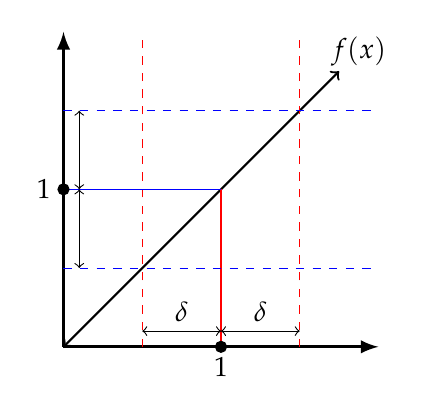
\begin{tikzpicture}[scale=2]
        \draw[-latex,very thick] (0,0)--(2,0);
        \draw[-latex,very thick] (0,0)--(0,2);
        \draw[<->, thick] (0, 0) -- (1.75, 1.75);
        \draw[color = red] (1, 0) -- (1, 1);
        \draw[color = red, dashed] (0.5, 0) -- (0.5, 2);
        \draw[color = red, dashed] (1.5, 0) -- (1.5, 2);
        \draw[<->] (0.5, 0.1) -- (1, 0.1);
        \node[above] at (0.75, 0.1) {$\delta$};
        \draw[<->] (1, 0.1) -- (1.5, 0.1);
        \node[above] at (1.25, 0.1) {$\delta$};
        \draw[color = blue] (0, 1) -- (1, 1);
        \draw[color = blue, dashed] (0, 0.5) -- (2, 0.5);
        \draw[color = blue, dashed] (0, 1.5) -- (2, 1.5);
        \draw[<->] (0.1, 0.5) -- (0.1, 1);
        \node[right] at (0.1, 0.75) {$\e$};
        \draw[<->] (0.1, 1) -- (0.1, 1.5);
        \node[right] at (0.1, 1.25) {$\e$};
        \draw[fill = black] (0, 1) circle (1pt);
        \node[xshift = -0.25cm] at (0, 1) {$1$};
        \draw[fill = black] (1, 0) circle (1pt);
        \node[yshift = -0.25cm] at (1, 0) {$1$};
        \node[yshift = 0.25cm, xshift = 0.25cm] at (1.75, 1.75) {$f(x)$};
    \end{tikzpicture}
    \caption{Visualization of the limit $\lim_{x \rightarrow 1}f(x) = 1$ for $f(x) = x$. For any $\e > 0$, we can take $\delta = \e$ and then we have that $\abs{f(x) - 1} < \e$ if $\abs{x - 1} < \delta$.}
    \label{fig17}
\end{figure}
Note in the above definition that we do not care about $f(p)$, that is, the actual value of $f$ at $p$. In particular, if $p \notin E$, then $f(p)$ is not even necessarily defined. This distinction between the limit and the actual value of a function at a point becomes crucial later on when we want to define a derivative. Although we will discuss this in more detail in Chapter 5, the definition of a derivative of a function $g$ at a point $p \in \RR$ involves the function $f: \RR \rightarrow \RR$ such that:
\begin{align*}
    f(x) = \frac{g(x) - g(p)}{x - p}
\end{align*}
Evidently, the domain of $f$ does not contain the point $p$, but we are interested in the value of $f$ in the limit of $x \rightarrow p$ (which, if it exists, is the value of the derivative).

\begin{figure}[htbp]
    \centering
    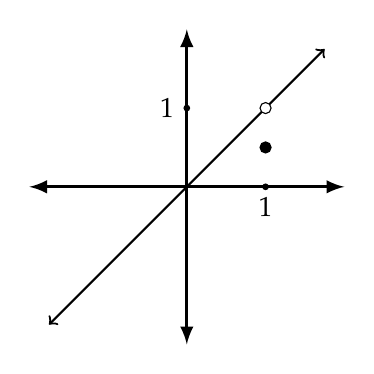
\begin{tikzpicture}
        \draw[latex-latex,very thick] (-2,0)--(2,0);
        \draw[latex-latex,very thick] (0,-2)--(0,2);
        \draw[<->, thick] (-1.75, -1.75) -- (1.75, 1.75);
        \draw[fill = black] (0, 1) circle (1pt);
        \node[xshift = -0.25cm] at (0, 1) {$1$};
        \draw[fill = black] (1, 0) circle (1pt);
        \node[yshift = -0.25cm] at (1, 0) {$1$};
        \draw[fill = white] (1, 1) circle (2pt);
        \draw[fill = black] (1, 0.5) circle (2pt);
    \end{tikzpicture}
    
    \caption{Visualization of the function $f(x) = x$ for $x \in \RR \setminus \set{1}$, $f(x) = 0$ for $x = 1$. In this case, we have that $f(1) = 0$ but $\lim_{x \rightarrow 1} f(x) = 1$, demonstrating that the actual value of the function is irrelevant when defining the limit.}
    \label{fig18}
\end{figure}

\begin{theorem}{}{4.2}
    Let $X, Y$ be metric spaces. Let $E \subset X$ and $f:E \mapsto Y$. Suppose that for all sequences $\set{p_n} \subset E$ with $p_n \rightarrow p$ and $p_n \neq p$, we have that $f(p_n) \rightarrow q \in Y$. Then, this is equivalent to saying that $\lim_{x \rightarrow p} f(x) = q$.
\end{theorem}
\begin{nproof}
    \boxed{\implies} Suppose that $\lim_{x \rightarrow p} f(x) = q$, and let $\set{p_n}$ be a sequence in $E$ with $p_n \rightarrow p$ and $p_n \neq p$ for all $n$. We wish to show that $f(p_n) \rightarrow q$. Let $\e > 0$. We show that there exists $N \in \NN$ such that $d_Y(f(p_n), q) < \e$ for all $n \geq N$. Since $\lim_{x \rightarrow p} f(x) = q$, there exists $\delta > 0$ such that for all $x \in E$ with $d_X(p, x) < \delta$, $d_Y(f(x),q) < \e$. Since we know that $p_n \rightarrow p$, there exists some $N$ such that $0 < d(p_n, p) < \delta$ for all $n \geq N$, so we have that $d_Y(f(p_n), q) < \e$ as required. 

    \boxed{\impliedby} We show the contrapositive. Suppose that $\lim_{x \rightarrow p} f(x) \neq q$. We wish to find a sequence $\set{p_n} \subset E$ with $p_n \rightarrow p$ and $p_n \neq p$ for all $n$ such that $f(p_n)$ does not converge to $q$. Since $\lim_{x \rightarrow p} f(x) \neq q$, then there exists $\e > 0$ such that for all $\delta > 0$, there exists $x \in E$ such that $0 < d_X(x, p) < \delta$ but $d_Y(f(x), q) \geq \e$. For each $\delta$ of the form $\frac{1}{n}$, let $p_n \in E$ be the corresponding value of $x$. Then, $p_n \rightarrow p$, $p_n \neq p$ for all $n$, and $f(p_n)$ does not converge to $q$ as $d(f(p_n), q) \geq \e$ for all $n$. \qed
\end{nproof}

\stepcounter{rudin}

\begin{theorem}{}{4.4}
    When $Y = \CC$ (i.e. the functions we consider are complex), then limits respect sums, differences, products, and functions. That is, let $X$ is a metric space, $E \subset X$, and $f, g: E \mapsto \CC$ with $p$ a limit point of $E$. If $\lim_{x \rightarrow p}f(x) = q$ and $\lim_{x \rightarrow p}g(x) = r$, then $\lim_{x \rightarrow p}(f+g)(x) = q + r$. The same holds for subtraction, multiplication, and division (provided we do not divide by zero).
\end{theorem}
\begin{nproof}
    By Theorem \ref{thm:4.2}, these properties of limits follow from the analogous properties of sequences (Theorem \ref{thm:3.3}).
\end{nproof}

\begin{definition}{Continuity}{4.5}
    Let $X, Y$ be metric spaces, and $E \subset X$. Let $p \in E$, and define $f: E \mapsto Y$. We say that $f$ is \textbf{continuous} at $p$ if for all $\e > 0$, there exists $\delta > 0$ such that for all $x \in E$ with $d_X(x, p) < \delta$, we have that $d_Y(f(x), f(p)) < \e$. Equivalently, $f(N_\delta^E(p)) \subset N_\e^Y(f(p))$. If $f$ is continuous at $p$ for all $p \in E$, we say that $f$ is continuous.
\end{definition}
\noindent Note that this definition of continuity is heavily reliant on the particular metric of $X$ and $Y$; in particular, there can be functions that are continuous for some choices of metric but not others.

Let us consider some examples of continuous functions (while thinking about different possible metric spaces). 

First, let us take onsider $X = E = \ZZ$ and $Y = \RR$. What functions $f: E \rightarrow Y$ are continuous at $p = 0$? The answer turns out to be all functions! To see this, fix $n \in \ZZ$ and let $\e > 0$. We then have that if $\abs{n - m} < \frac{1}{2}$, then $\abs{f(n) - f(m)} < \e$ as the only point $m$ contained in $N_{1/2}^\ZZ(n)$ is $n$ itself (and hence $\abs{f(n) - f(m)} = \abs{f(n) - f(n)} = 0$). This argument applies to every $n \in \ZZ$ and hence all functions $f: \ZZ \mapsto \RR$ are continuous.

As further examples (that work for arbitrary metric spaces), If we have that $f: X \mapsto X$, $f(x) = x$, we have that $f$ is continuous (pick $\delta = \e$ in the definition of continuity). If we have that $f: X \mapsto Y$, $f(x) = c$ for some $c \in Y$, then $f$ is also continuous (pick any $\delta > 0$ in the definition). 

Finally, the above definition doesn't make a distinction between limit points and isolated points. However, it turns out that according to the definition, if $p \in E$ is isolated, then every function $f$ with $E$ as its domain is continuous. To see this, consider that for any $\e > 0$, we can pick $\delta > 0$ such that the only point $x \in E$ for which $d_X(x, p) < \delta$ is $x = p$ (such a choice of $\delta$ is possible as $p$ is isolated). It then follows that $d_Y(f(x), f(p)) = 0 < \e$. 
 
We now consider a Theorem which gives us a familiar notion of continuity (that may have been encountered in first year calculus).

\begin{theorem}{}{4.6}
    Suppose that $p$ is a limit point of $E$ in Definition \ref{def:4.5}. Then, $f$ is continuous at $p$ if and only if $\lim_{x \rightarrow p}f(x) = f(p)$. 
\end{theorem}
\begin{nproof}
    The claim immediately follows by comparing Definitions \ref{def:4.1} and \ref{def:4.5}. \qed
\end{nproof}

\begin{theorem}{}{4.7}
    Let $X, Y, Z$ be metric spaces, and $E \subset X, F \subset Y$. Let $f: E \mapsto Y$, $g: F \mapsto Z$, and suppose $f(E) \subset F$. Let $p \in E$. If $f$ is continuous at $p$ and $g$ is continous at $f(p)$, then $g \circ f: E \mapsto Z$ is continuous at $p$.
\end{theorem}
\begin{nproof}
    Let $\e > 0$. Since $g$ is continuous at $f(p)$, there exists $\gamma > 0$ such that $d_Z(g(y), g(f(p))) < \e$ if $d_Y(y, f(p)) ,< \gamma$. Since $f$ is continuous at $p$, there exists $\delta > 0$ such that $d_Y(f(x), f(p)) < \gamma$ if $d_X(x, p) < \delta$. Hence, we have that $d_Z(h(x), h(p)) = d_Z(g(f(x)), g(f(p))) < \e$ if $d_X(x, p) < \delta$ and $x \in E$. We conclude that $h$ is continuous at $p$. \qed
\end{nproof}

\subsection{Topological Characterization of Continuity}
\begin{theorem}{}{4.8}
    Let $X, Y$ be metric spaces, and $f: X \mapsto Y$. Then, $f$ is continuous if and only if $f^{-1}(V) \subset X$ is open for every open set $V \subset Y$.
\end{theorem}
\begin{nproof}
    \boxed{\implies} Suppose $f$ is continuous, and $V \subset Y$ is open. Let $p \in f^{-1}(V)$, so $f(p) \in V$. $V$ is open, so it follows that $f(p)$ is an interior point of $V$. So, there exists $r > 0$ such that $N_r^Y(f(p)) \subset V$. Next, $f$ is continuous, so there exists $\delta > 0$ such that for all $x \in X$ with $d_X(x, p) < \delta$, $d_Y(f(x), f(p)) < r$. Hence, we obtain that $f(x) \in N_r^Y(f(p)) \subset V$. In particular, $N_\delta^X(p) \subset f^{-1}(V)$, so $p$ is an interior point of $f^{-1}(V)$. Hence every point of $f^{-1}(V)$ is an interior point, and $f^{-1}(V)$ is open.

    \boxed{\impliedby} Suppose $f^{-1}(V)$ is open for every open set $V \subset Y$. Let $p \in X$ and $\e > 0$. Let $V = N_\e^Y(f(p))$ which is open, so by assumption $f^{-1}(V)$ is open. $p \in f^{-1}(V)$, so $p$ is an interior point. Hence, there exists $\delta > 0$ such that $N_\delta^X(p) \subset f^{-1}(V)$. In other words, if $d_X(x, p) < \delta$, then $f(x) \in V$, so $d_Y(f(x), f(p)) < \e$. $f$ is then continuous by definition. \qed
\end{nproof}

\begin{ncorollary}{}{}
    $f: X \mapsto Y$ is continuous if and only if $f^{-1}(F) \subset X$ is closed for every closed set $F \subset Y$.
\end{ncorollary}
\begin{nproof}
    Let $V = F^c$ with $V$ open. Then, the above statement is equivalent to saying that a function $f: X \mapsto Y$ is continuous if and only if $f^{-1}(V^c) = \left(f^{-1}(V)\right)^c$ is closed for every open set $V \subset Y$. This is equivalent to the statement that $f^{-1}(V)$ is open for every open set $V \subset Y$, and the claim follows by the previous theorem. \qed
\end{nproof}

\noindent Note that the above topological characterization says properties of sets are preserved under taking the preimage; it does not say anything about preserving properties under the image. That is to say, images of open/closed sets are not necessarily open/closed.

\begin{nexample}{}{}
    Consider $X = \RR^+ = (0, \infty)$ and $Y = \RR$. Then, the function:
    \begin{align*}
        \fullfunction{f}{X}{Y}{x}{\frac{1}{x}}
    \end{align*}
    is continuous. Then defining $A = [1, \infty)$ we have that $A$ is closed, but $f(A) = (0, 1]$ is not closed.   
\end{nexample}


\begin{theorem}{}{4.9}
    Let $f: X \mapsto \CC$ and $g: X \mapsto \CC$ be continous functions. Then, $f+g$, $fg$ are continuous, and $\frac{f}{g}$ is continuous if $g(x) \neq 0$. 
\end{theorem}
\begin{nproof}
    At isolated points there is nothing to prove (as any choice of function that is defined at an isolated $p$ will be continuous there). For limit points, the claim follows from Theorems \ref{thm:4.4} and \ref{thm:4.6}. \qed
\end{nproof}

\begin{theorem}{}{4.10}
    \begin{enumerate}
        \item Let $f_1, f_2, \ldots, f_k: X \mapsto \RR$, and define $\v{f}: X \mapsto \RR^k$ by:
        \begin{align*}
            \v{f}(x) = (f_1(x), f_2(x), \ldots, f_k(x))
        \end{align*}
        Then, $\v{f}$ is continuous if and only if every $f_i$ is continuous.
        \item If $\v{f} = (f_1, \ldots f_k): X \mapsto \RR^k$ and $\v{g} = (g_1, \ldots g_k): X \mapsto \RR^k$ are continous, then the functions:
        \begin{align*}
            \v{f} + \v{g} = (f_1 + g_1, \ldots, f_k + g_k)
        \end{align*}
        \begin{align*}
            \v{f} \cdot \v{g} = f_1g_1 + \ldots + f_kg_k
        \end{align*}
        are continous.
    \end{enumerate} 
\end{theorem}
\begin{nproof}
    \begin{enumerate}
        \item $\boxed{\implies}$ Suppose $\v{f}$ is continuous. Then, let $\e > 0$. For each $p \in X$, there exists $\delta > 0$ such that $d_X(x, p) < \delta$ implies $\abs{\v{f}(x) - \v{f}(p)} < \e$. We then observe that for any $i \in \set{1, \ldots k}$:
        \begin{align*}
            \abs{\v{f}(x) - \v{f}(p)} = \left(\sum_{j=1}^k \abs{f_j(x) - f_j(p)}^2\right)^{1/2} \geq \abs{f_i(x) - f_i(p)}
        \end{align*}
        Where the inequality follows by just keeping one term from the sum of non-negative terms. So for any $d_X(x, p) < \delta$ we therefore have that $\abs{f_i(x) - f_i(p)} < \e$, and hence each $f_i$ is continuous.
        
        $\boxed{\impliedby}$ Suppose each of $f_1, \ldots f_k$ is continuous. Then let $\frac{\e}{\sqrt{k}} > 0$. For each $p \in X$, there exists $\delta_i$ such that $d_X(x, p) < \delta_i$ implies that $\abs{f_i(x) - f_i(p)} < \frac{\e}{\sqrt{k}}$. Take $\delta = \min\set{\delta_1, \ldots \delta_k}$. Then, if $d_X(x, p) < \delta$, we have that:
        \begin{align*}
            \abs{\v{f}(x) - \v{f}(p)} = \left(\sum_{j=1}^k \abs{f_j(x) - f_j(p)}^2\right)^{1/2} < \left(\sum_{j=1}^k \left(\frac{\e}{\sqrt{k}}\right)^2\right)^{1/2} = \e
        \end{align*}
        So it follows that $\v{f}$ is continuous.
        \item The claim follows from (a) and Theorem \ref{thm:4.9}. \qed
    \end{enumerate}
\end{nproof}

\begin{example}{}{4.11}
    We will now explore some interesting examples of continuous functions.
    \begin{enumerate}
        \item For each index $i = 1, \ldots k$, define $\phi_i: \RR^k \mapsto \RR$ by $\phi_i(\v{x}) = x_i$. Then, $\phi_i$ is continuous.
        \begin{proof}
            Let $\e > 0$. Then, for $\v{p} \in \RR^k$, if $\abs{\v{x} - \v{p}} < \delta$ with $\delta = \e$, we have that:
            \begin{align*}
                \e > \abs{\v{x} - \v{p}} = \left(\sum_{j=1}^k \abs{x_j - p_j}^2\right)^{1/2} \geq \left(\abs{x_i - p_i}^2\right)^{1/2} = \abs{x_i - p_i}
            \end{align*}
            So for $\abs{\v{x} - \v{p}} < \delta$, we have that $\abs{\phi_i(\v{x}) - \phi_i(\v{p})} < \e$. We conclude that $\phi_i$ is continous.
        \end{proof}
        We could also use the topological characterization of continuity to prove this claim. If $V \subset \RR$ is open, then $\RR \times \RR \times \ldots \times V \times \RR \times \ldots \times \RR$ is open, showing again that $\phi_i$ is continuous (a much easier proof)!
        \item Let $f: \RR^k \mapsto \RR$ be given by $f(\v{x}) = x_1^{n_1}x_2^{n_2}\cdots x_k^{n_k}$ with $n_i \in \NN \cup \set{0}$. $f$ is continous, and hence so is any polynomial $P: \RR^k \mapsto \RR$.
        \item Rational functions $P/Q$ where $P, Q$ are polynomials are continous everywhere except where $Q$ is zero.
        \item $f: \RR^k \mapsto \RR$ given by $f(\v{x}) = \abs{\v{x}}$ is continous.
        \item Suppose $f: X \mapsto \RR^k$ is continous. Then so is $g: X \mapsto \RR^k$ with $g(x) = \abs{f(x)}$.
    \end{enumerate}
\end{example}

\subsection{Continuity and Compactness}

\setcounter{rudin}{13}
\begin{theorem}{}{4.14}
    Let $f: X \mapsto Y$ be continuous, and suppose $X$ is compact. Then, the image $f(X)$ is compact.
\end{theorem}
\begin{nproof}
    Let $\set{V_\alpha}$ be an open cover of $f(X)$. For each $\alpha$, Let $O_\alpha = f^{-1}(V_\alpha)$. Then, $\set{O_\alpha}$ is an open cover of $X$. to see this, we recognize that each $O_\alpha$ is open due to the continuity of $f$ (Theorem \ref{thm:4.8}) and each $p \in X$ satisfies $V_\beta$ for some $\beta$, so $p \in O_\beta$. $X$ is compact, so there exists a finite subcover $\set{O_{\alpha_1}, \ldots O_{\alpha_n}}$. But it then follows that $\set{V_{\alpha_1}, \ldots V_{\alpha_n}}$ is a finite subcover of $f(X)$. Hence $f(X)$ is compact. \qed
\end{nproof}
\noindent We previously discussed how an image of a closed set (under a continuous function) does not have to be closed. However, the above Theorem shows that the image of a compact set (under a continuous function) must be compact.

Taking a slight tangent, a question of interest may be to consider the topology of the extended real numbers; namely, $\RR \cup \set{\infty, -\infty}$ (where $-\infty < x < \infty$ for all $x \in \RR$). In particular, a natural question to ask is whether $[1, \infty) \cup \set{\infty}$ would be closed/compact.

We start then by defining a reasonable metric on $X = \RR \cup \set{\infty, -\infty}$. A ``reasonable'' definition of a metric will satify the requirement that $[1, \infty) \cup \set{\infty}$ is compact or not. We then define the metric:
\begin{align*}
    d(x, y) = \abs{\arctan(x) - \arctan(y)}
\end{align*}
where $\arctan(\infty) = \frac{\pi}{2}$ and $\arctan(-\infty) = -\frac{\pi}{2}$. We then have that $(X, d)$ is a metric space (check!) 

Note that the extended reals have been made into a metric space here, but it is no longer a field; in particular, we have that $(-\infty + \infty) + \infty = 0 + \infty = \infty$ but $-\infty + (\infty + \infty) = -\infty + \infty = 0$ so associativity no longer holds.

With a reasonable metric defined on the extended reals, let us now return to our previous example in Section 4.2 where we considered the function $f(x) = \frac{1}{x}$. We now extend the domain of the function such that:
\begin{align*}
    \fullfunction{f}{X \setminus \set{0}}{\RR}{x}{\frac{1}{x}}
\end{align*}
With $f(\infty) = f(-\infty) = 0$. We leave it as an exercise to verify that $f$ is continuous on $X \setminus \set{0}$ using the continuity of the $\arctan$ function. 

Now, consider $A = [1, \infty) \subset X$. $A$ is not closed, as $\infty$ is a limit point of $A$ (this can be verified by checking that for all $\e > 0$, there exists $x \in [1, \infty)$ such that $\abs{\arctan x - \arctan \infty} = \frac{\pi}{2} - \arctan x < \e$). However, we do have that $\overline{A} = [1, \infty]$ is closed and compact, and that $f(\overline{A}) = [0, 1]$ is compact as Theorem \ref{thm:4.14} states. In a sense, we have ``compactified'' the reals through our construction, as $X$ is compact while $\RR$ was not. We also have that $X$ is bounded (unlike $\RR$), as all distances between points are bounded by at most $\pi$. In particular, $\diam X = \pi$. 


\setcounter{rudin}{12}
\begin{definition}{Bounded functions}{4.13}
    Let $X$ be a metric space, and $E \subset X$. We say that $f: E \mapsto Y$ is \textbf{bounded} if $f(E)$ is a bounded set. In particular, if $Y = \RR^k$, then $f$ is bounded if and only if there exists $M \in \RR$ such that $\abs{f(x)} \leq M$ for all $x \in E$.
\end{definition}

\setcounter{rudin}{14}
\begin{theorem}{}{4.15}
    Let $X$ be a compact metric space, and $f: X \mapsto Y$ be continuous. Then, $f(X)$ is bounded.
\end{theorem}
\begin{nproof}
    By Theorem \ref{thm:4.14}, we have that $f(X)$ is compact. $f(X)$ is therefore bounded (see discussion proceeding Theorem \ref{thm:2.41}). \qed
\end{nproof}
\noindent An interesting special case in the above theorem to think about is when $Y = \RR$; this yields the Extreme Value Theorem, below.

\begin{theorem}{Extreme Value Theorem}{4.16}
    Let $X$ be a compact metric space, and let $f: X \mapsto \RR$ be continuous. Then, there exist $p, q \in X$ such that $f(p) \leq f(x) \leq f(q)$ for all $x \in X$. In other words, $f$ attains its minimum (infimum) and maximum (supremum) on $X$.
\end{theorem}
\begin{nproof}
    By Theorems \ref{thm:4.15} and \ref{thm:4.16}, $f(X)$ is closed and bounded. In particular, $m = \inf f(X)$ and $M = \sup f(X)$ exist (as the set is bounded), and $m, M \in f(X)$ as $f(X)$ contains all of its limit points. Hence, there exist $p, q \in X$ such that $f(p) = m$, $f(q) = M$. \qed
\end{nproof}

\begin{theorem}{}{4.17}
    Let $X$ be a compact metric space, and $f: X \mapsto Y$ be continuous and a bijection. Define $f^{-1}: Y \mapsto X$ by $f^{-1}(y) = x$ if $f(x) = y$ (this is well-defined due to the bijectivity of $f$). Then, $f^{-1}$ is continuous.
\end{theorem}
\begin{nproof}
    By Theorem \ref{thm:4.8}, it suffices to show that for every open set $V \subset X$, $\left(f^{-1}\right)^{-1}(V) = f(V)$ is open. By the openness of $V$, $V^c$ is closed, and hence compact (as closed subsets of compact sets are compact by Theorem \ref{thm:2.35}). So, $f(V^c) \subset Y$ is compact by Theorem \ref{thm:4.14}. Therefore, $f(V^c) = \left(f(V)\right)^c$ is closed (as compact sets are closed by Theorem \ref{thm:2.34}). Therefore, $\left(\left(f(V)\right)^c\right)^c = f(V)$ is open as desired. Hence $f^{-1}$ is continuous. \qed
\end{nproof}

\setcounter{rudin}{20}
\begin{example}{}{4.21}
    This example shows the necessity of compactness of $X$ in Theorem \ref{thm:4.17}. Let $S = [0, 2\pi)$ which is not closed and hence not compact (Heine Borel/Theorem \ref{thm:2.41}). Let $Y = \set{(x, y) \in \RR^2: x^2 + y^2 = 1}$. Define $f: X \mapsto Y$ where $f(\theta) = (\cos\theta, \sin\theta)$. $f$ is continuous and a bijection (check!) but $f^{-1}$ is not continuous. To see this is the case, consider first that $[0, \frac{\pi}{2}) \subset X$ is open in $X$. At everywhere except $0$ it should be evident that all points of $[0, \frac{\pi}{2})$ are interior to $X$, and at $0$, we have that $N_{1/2}(0) \subset [0, \frac{\pi}{2})$ showing that $0$ is also an interior point. But, $(f^{-1})^{-1}([0, \frac{\pi}{2})) = f([0, \frac{\pi}{2}))$ is not open, because not every point is an interior point; namely, $(1, 0) = f(0) \in f([0, \frac{\pi}{2}))$ is not an interior point. So, $f^{-1}$ is not continuous.
\end{example}

\begin{figure}[htbp]
    \centering
    \begin{tikzpicture}[scale=2]
        \foreach \i in {-2.95,-2.9,...,-2.5}{ 
            \draw[blue] (\i,0.05) -- (\i,-0.05);
            }
        \begin{scope}[shift={(0:2)}]
        \foreach \i [count=\j] in {0, 2, 4,...,90} {
            \draw[blue] (\i:1) -- (\i:1.11);
            }
        \end{scope}
        \draw[] (-3, 0) -- (-1, 0);
        \node[] at (-3, 0) {$[$};
        \node[] at (-1, 0) {$)$};
        \node[below] at (-3, -0.25) {$0$};
        \node[below] at (-1, -0.25) {$2\pi$};
        \draw[->, thick] (-0.5, 0) -- (0.5, 0);
        \node[above] at (0, 0) {$f$};
        \draw[] (2, 0) circle (30pt);
        \node[] at (-2.5, 0) {$)$};
        \node[below] at (-2.5, -0.25) {$\frac{\pi}{2}$};
        \node[rotate = 270] at (3.05, 0) {$]$};
        \node[] at (2, 1.05) {$($};
    \end{tikzpicture}
    
    \caption{Visual of the map $f$ which maps a point $\theta \in [0, 2\pi)$ to the point $(\cos\theta, \sin\theta)$ on the unit circle. Pictured is the map from $[0, \frac{\pi}{2})$ to $f([0, \frac{\pi}{2}))$, the former which is open in $[0, 2\pi)$, and the latter which is not open in $Y = \set{(x, y) \in \RR^2: x^2 + y^2 = 1}$.}
    \label{fig19}
\end{figure}

\subsection{Uniform Continuiity, Connectedness, and IVT}

\setcounter{rudin}{17}
\begin{definition}{Uniform Continuity}{4.18}
    Let $X, Y$ be metric spaces and $f: X \mapsto Y$. Then, $f$ is \textbf{uniformly continuous} if for all $\e > 0$, there exists $\delta > 0$ such that for all $p, q \in X$ with $d_X(p, q) < \delta$, we have that $d_Y(f(p), f(q)) < \e$. It is clear from the definition that every uniformly continuous function is continuous.
\end{definition}
\noindent Note that this definition is very similar to the definition of continuity, but with a difference in the quantifiers. With continuity, for each $\e$ there is a $\delta$ that we can find for a given point $p \in X$. For uniform continuity, we have that for each $\e$, there exists a $\delta$ that works uniformly for all $p$. 

We now consider some examples to see the difference concretely. Take $X = (0, 1), Y = \RR$, and $f(x) = \frac{1}{x}$. We then have that $f$ is continuous, but not uniformly continuous, showing that in general continuity does not imply uniform continuity.

Next, consider $X = Y = \RR$ and $f(x) = \sin x$. Then, $f$ is uniformly continuous. Given any $\e$, we can pick $\delta = \e$ and this proof will work. The ``calclus-inspired'' proof would use that $\od{}{x}\sin x = \cos x$ and $\abs{\cos x} \leq 1$, so we can always pick $\delta = \e$ with the MVT. However, we have yet to define the derivative or prove the mean value theorem, so an alternate appraoch would be to invoke trigonometric identities.

Finally, let $X = [0, 10], Y = \RR$, and $f(x) = x^2$. Then, $f$ is uniformly continuous. However, if $X = Y = \RR$ and $f(x) = x^2$, then $f$ is not uniformly continuous. The uniform continuity of $f$ depends on the domain; in particular, $[0, 10]$ is closed/compact, while $\RR$ is not compact. This motivates our next theorem.

\begin{theorem}{}{4.19}
    Let $X, Y$ be metric spaces with $X$ compact. Let $f: X \mapsto Y$ be continuous. Then, $f$ is uniformly continuous.
\end{theorem}
\begin{nproof}
    Let $\e > 0$. By the continuity of $f$, for each $p \in X$, there exists $\delta_p  0$ such that for all $q \in X$ with $d_X(p, q)  <\delta_p$, we have that $d_Y(f(p), f(q)) < \frac{\e}{2}$. Define $U_p = N_{\delta_p/2}(p)$. We then have that $\set{U_p}_{p \in X}$ is an open cover for $X$. By the compactness of $X$, it has a finite subcover. Let $\set{U_{p_1}, \ldots, U_{p_n}}$ be a finite subcover. Let $\delta = \frac{1}{2}\min\set{\delta_{p_1}, \ldots, \delta_{p_n}} > 0$ (note the importance of taking the minimum over a \textit{finite} number of $\delta_{p_i}$s; if we took an infimum over an infinite number, it could be possible that the infimum could be zero). Then, take $p, q \in X$ with $d_X(p, q) < \delta$. Then, $p \in U_{p_i}$ for some $i$. So, $d_X(p, p_i) < \frac{\delta_{p_i}}{2}$, and then by the triangle inequality we have that:
    \begin{align*}
        d_X(q, p_i) \leq d_X(q, p) + d_X(p, p_i) < \delta + \frac{\delta_{p_i}}{2} \leq \frac{\delta_{p_i}}{2} + \frac{\delta_{p_i}}{2} = \delta_{p_i}
    \end{align*} 
    Therefore, we have that:
    \begin{align*}
        d_Y(f(p), f(q)) \leq d_Y(f(p), f(p_i)) + d_Y(f(p_i), f(q)) < \frac{\e}{2} + \frac{\e}{2} = \e
    \end{align*}
    And we conclude that $f$ is uniformly continuous. \qed
\end{nproof}

\setcounter{rudin}{21}
\begin{theorem}{}{4.22}
    Let $X, Y$ be metric spaces, and let $f: X \mapsto Y$ be continuous. If $E \subset X$ is connected (see Definition \ref{def:2.45}) then its image $f(E)$ is also connected.
\end{theorem}
\begin{nproof}
    Suppose for the sake of contradiction that we can write $f(E) = A \cup B$ with $A, B \neq \emptyset$ and $A \cap \overline{B} = \overline{A} \cap B = \emptyset$ (i.e. $f(E)$ is not connected). Then, define $G = f^{-1}(A) \cap E$ and $H = f^{-1}(B) \cap E$. Then, $E = G \cup H$, with $G \neq \emptyset$, $H \neq \emptyset$, and $G \cap H = \emptyset$. We wish to show that $\overline{G} \cap H = G \cap \overline{H} = \emptyset$ as this will contradict the connectedness of $E$. Since $A \subset \overline{A}$, We have that $G \subset f^{-1}(A) \subset f^{-1}(\overline{A})$. $f$ is continuous, so by Theorem \ref{thm:4.8}, we have that $f^{-1}(\overline{A})$ is closed. Hence by Theorem \ref{thm:2.27} we have that $\overline{G} \subset f^{-1}(\overline{A})$. Since $f(H) = B$ and $\overline{A} \cap B = \emptyset$, we have that:
    \begin{align*}
        f(\overline{G}) \cap f(H) = \emptyset
    \end{align*}
    And therefore $\overline{G} \cap H = \emptyset$. By an identitcal argument, $G \cap \overline{H} = \emptyset$. Hence, $E = G \cup H$ is not connected, which is a contradiction. \qed
\end{nproof}

\begin{theorem}{Intermediate Value Theorem}{4.23}
    Let $f: [a, b] \mapsto \RR$ be continuous and $f(a) < f(b)$. Then, for all $\alpha \in (f(a), f(b))$, there exists $c \in (a, b)$ with $f(c) = \alpha$.
\end{theorem}
\begin{nproof}
    $[a, b]$ is connected, so by Theorem \ref{thm:4.22}, $f([a, b])$ is conected. Hence by \ref{thm:2.47}, it contains every point between $f(a)$ and $f(b)$. \qed
\end{nproof}

\begin{figure}[htbp]
    \centering
    \begin{tikzpicture}[scale=2]
        \draw[-latex] (-2.5, 0) -- (-2.5, 2);
        \draw[-latex] (-2.5, 0) -- (-0.5, 0);
        \draw [] (-2.25 , 0.5) to [ curve through ={(-2, 0.75)..(-1.75, 1.1)..(-1.5, 1.25)..(-1.25,1.6)}] (-1,1.5);
        \filldraw[] (-2.25, 0.5) circle (1pt);
        \filldraw[] (-1, 1.5) circle (1pt);
        \draw[dashed] (-2.5, 1.25) -- (-1.5, 1.25);
        \draw[] (-2.25, 0) -- (-2.25, -0.15);
        \node[below] at (-2.25, -0.16) {$a$};
        \draw[] (-1, 0) -- (-1, -0.15);
        \node[below] at (-1, -0.13) {$b$};
        \draw[] (-1.5, 0) -- (-1.5, -0.15);
        \node[below] at (-1.5, -0.17) {$c$};
        \node[left] at (-2.5, 1.25) {$\alpha$};
        \draw[-latex] (0.5, 0) -- (0.5, 2);
        \draw[-latex] (0.5, 0) -- (2.5, 0);
        \draw[] (0.75, 0.5) -- (1.375, 0.5);
        \draw[] (1.375, 1.5) -- (2, 1.5);
        \filldraw[] (0.75, 0.5) circle (1pt);
        \draw[fill = white] (1.375, 0.5) circle (1pt);
        \filldraw[] (1.375, 1.5) circle (1pt);
        \filldraw[] (2, 1.5) circle (1pt);
        \draw[] (0.75, 0) -- (0.75, -0.15);
        \node[below] at (0.75, -0.16) {$a$};
        \draw[] (2, 0) -- (2, -0.15);
        \node[below] at (2, -0.13) {$b$};
    \end{tikzpicture}
    
    \caption{Visualization of functions for which the IVT applies (left) and for which it doesn't (right).}
    \label{fig20}
\end{figure}
\newpage
\section[Differentiation]{\hyperlink{toc}{Differentiation}}

\subsection{Derivatives}
\begin{definition}{Derivatives}{5.1}
    Let $f: [a, b] \mapsto \RR$, and $x \in [a, b]$. We then define the \textbf{derivative} of $f$ at $x$ as:
    \begin{align*}
        f'(x) = \lim_{t\rightarrow x} \frac{f(t) - f(x)}{t - x}
    \end{align*}
    If the limit exists. Alternative notations for the derivative are given by:
    \begin{align*}
        \dpd{f}{x}(x) \text{ or } \dod{}{x}f(x) \text { or } \left.\dod{}{y}f(x)\right|_{y = x}
    \end{align*}
\end{definition}
As an interpretation of the derivative, take $[a, b]$ to be a metric space, with $x$ a limit point of $[a, b] \setminus \set{x}$. Then, $g(t) = \frac{f(t) - f(x)}{t - x}$ is a function from $[a, b] \setminus \set{x} \mapsto \RR$. If $x \in (a, b)$, then the above definition of the derivative agrees with the definition of $f'(x)$ from first year calculus. If $x = a$ or $x = b$, then the above definition agrees with the definition of the one-sided derivative from first year calculus. Note that we will not discuss in this class cases where the domain gets more complicated (i.e. not just closed intervals of $\RR$).

\begin{theorem}{}{5.2}
    Let $f:[a,b] \mapsto \RR$, let $x \in [a, b]$, and suppose $f'(x)$ exists. Then, $f$ is continuous at $x$.
\end{theorem}
\begin{nproof}
    For $t \neq x$, we can write:
    \begin{align*}
        f(t) = f(x) + (f(t) - f(x)) = f(x) + \frac{f(t) - f(x)}{t - x}(t - x)
    \end{align*}
    Taking the limit of $t \rightarrow x$, we then have that:
    \begin{align*}
        \lim_{t \rightarrow x} f(t) = \lim_{t \rightarrow x} \left(f(x) + \frac{f(t) - f(x)}{t - x}(t - x) \right) = \lim_{t \rightarrow x} f(x) + \lim_{t \rightarrow x} \frac{f(t) - f(x)}{t - x} \lim_{t \rightarrow x} (t - x)
    \end{align*}
    Where in the last line we invoke Theorem \ref{thm:4.4}. Evaluating the limits on the RHS by using the existence of the derivative of $f$ at $x$, we have
    \begin{align*}
        \lim_{t \rightarrow x} f(t) = f(x) + f'(x)\cdot (0) = f(x)
    \end{align*}
    So we conclude that $f$ is continuous at $x$ by Theorem \ref{thm:4.6}. \qed
\end{nproof}
The interpretation is that differentiability at $x \in (a, b)$ implies continuity of $f$ at $x$, and the left/right differentiability of $f$ at $a/b$ implies the left/right continuity of $f$ at $a/b$. We have wrapped the proof of all these cases into one!

Note that the converse of the above theorem is not true. As a simple example, take $f(x) = \abs{x}$ on $[-1, 1]$, which is continuous at $x = 0$ (it can be verified that $\lim_{x \rightarrow 0}f(x) = f(0) = 0$) but is not differentiable there (the left/right handed limits of the difference quotient do not agree and hence the derivative does not exist). In Chapter 7, we will construct a function that is continuous everywhere and differentiable nowhere!

NWe will now proceed to prove a series of theorems that have been seen in first year, but using our new/rigorous definitions.

\begin{theorem}{Sum, Product, and Quotient Rules}{5.3}
    Let $f, g: [a, b] \mapsto \RR$. Let $x \in [a, b]$ and suppose $f$ and $g$ are differentiable at $x$. Then, $f + g$, $f - g$, $f\cdot g$ are differentiable at $x$, and so is $\frac{f}{g}$ provided $g(x) \neq 0$. Furthermore:
    \begin{enumerate}
        \item $(f+g)'(x) = f'(x) + g'(x)$
        \item $(fg)'(x) = f'(x)g(x) + f(x)g'(x)$
        \item $\left(\frac{f}{g}\right)'(x) = \frac{f'(x)g(x) - f(x)g'(x)}{(g(x))^2}$
    \end{enumerate}
\end{theorem}
\begin{nproof}
    \begin{enumerate}
        \item Follows immediately from the additive property of limits (Theorem \ref{thm:4.4}).
        \item Let $h = fg$. We then have that:
        \begin{align*}
            h(t) - h(x) = f(t)\left[g(t) - g(x)\right] + g(x)\left[f(t) - f(x)\right]
        \end{align*}
        For $t \neq x$, we can divide both sides by $t-x$ to obtain:
        \begin{align*}
            \frac{h(t) - h(x)}{t - x} = f(t)\frac{g(t) - g(x)}{t-x} + g(x)\frac{f(t) - f(x)}{t - x}
        \end{align*}
        Taking the limit of $t \rightarrow x$ on both sides, we obtain:
        \begin{align*}
            h'(x) = f(x)g'(x) + f'(x)g(x)
        \end{align*}
        as desired.
        \item Let $h(t) = \frac{f(t)}{g(t)}$. Then:
        \begin{align*}
            h(t) - h(x) &= \frac{f(t)}{g(t)} - \frac{f(x)}{g(x)}
            \\ &= \frac{1}{g(t)g(x)}\left(f(t)g(x) - g(t)f(x)\right)
            \\ &= \frac{1}{g(t)g(x)}\left[g(x)\left(f(t) - f(x)\right) - f(x)\left(g(t) - g(x)\right)\right]
        \end{align*}
        For $t \neq x$, we can divide both sides by $t - x$ to get:
        \begin{align*}
            \frac{h(t) - h(x)}{t - x} = \frac{1}{g(t)g(x)}\left[g(t)\frac{f(t) - f(x)}{t - x} - f(x)\frac{g(t) - g(x)}{t - x}\right]
        \end{align*}
        Taking the limit as $t \rightarrow x$ on both sides, we obtain the desired expression. \qed
    \end{enumerate}
\end{nproof}

\newpage 
\noindent As an exercise, one can prove by induction (applying 5.3(b)) that $(f_1f_2f_3\ldots f_n)'(x)$ (where $f_i: [a, b] \mapsto \RR$ and each $f_i'(x)$ exists) is given by:
\begin{align*}
    f_1'(x)f_2(x)\ldots f_n(x) + \cdots + f_1(x)f_2(x)\ldots f'_n(x).
\end{align*}
Note that as a corollary of this, we get that if $f(x) = x^n$, then $f'(x) = nx^{n-1}$ and we hence recover the familiar power rule from first year calculus!

\setcounter{rudin}{4}
\begin{theorem}{Chain Rule}{5.5}
    Let $f: [a, b] \mapsto \RR$, $x \in [a, b]$, and suppose $f$ is differentiable at $x$. Suppose furthermore that $f([a, b])$ is contained in some interval $I$. Let $g: I \mapsto \RR$ and suppose $g$ is differentiable at $f(x)$. Then, $g \circ f: [a, b] \mapsto \RR$ is differentiable at $x$, and furthermore:
    \begin{align*}
        (g \circ f)'(x) = g'(f(x))f'(x)
    \end{align*}
\end{theorem}
\begin{nproof}
    Define $h(t) = g \circ f(t)$ for $a \leq t \leq b$, $t \neq x$. We cna then write:
    \begin{align*}
        f(t) - f(x) = (t-x)\left[f'(x) + u(t)\right]
    \end{align*}
    For a function $u(t)$ with $\lim_{t \rightarrow x} u(t) = 0$. Now defining $y = f(x)$, we write:
    \begin{align*}
        g(s) - g(y) = (s-y)\left[g'(y) + r(s)\right]
    \end{align*}
    For a function $r(s)$ with $\lim_{s \rightarrow y}r(s) = 0$. Hence, we have that:
    \begin{align*}
        h(t) - h(x) &= g(f(t)) - g(f(x))
        \\ &= \left(f(t) - f(x)\right)\left(g'(y) + r(s)\right)
        \\ &= (t- x)\left[f'(x) + u(t)\right]\left(g'(y) + r(s)\right)
    \end{align*}
    Dividing both sides by $t - x$, we obtain:
    \begin{align*}
        \frac{h(t) - h(x)}{t - x} = \left[f'(x) + u(t)\right]\left(g'(y) + r(s)\right)
    \end{align*}
    We now take the limit of $t \rightarrow x$ on both sides. $\lim_{t \rightarrow x} u(t) = 0$, and $f$ is differentiable and hence continuous at $x$, so $s = f(t) \rightarrow y$ as $t \rightarrow x$. Thus, $r(s) \rightarrow 0$ as $t \rightarrow x$, and in conclusion:
    \begin{align*}
        h'(x) = (g \circ f)'(x) =  f'(x)g'(y) = g'(f(x))f'(x)
    \end{align*}
    as desired. \qed
\end{nproof}


\subsection{MVT}

\setcounter{rudin}{6}
\begin{definition}{Local Maxima/Minima}{5.7}
    Let $X$ be a metric space. Let $f: X \mapsto \RR$, and let $x \in X$. We say that $x$ is a \textbf{local maximum} of $f$ if there exists $\delta > 0$ such that $f(y) \leq f(x)$ for all $y \in N_{\delta}(x)$. A \textbf{local minimum} is defined similarly, with $f(y) \geq f(x)$ instead.
\end{definition}
\noindent For a metric space $X$ equipped with the discrete metric, all points $x \in X$ are simultaneously local maxima and minima. To see this, take any $0 < \delta \leq 1$. 

\begin{theorem}{}{5.8}
    Let $f: [a, b] \mapsto \RR$. Let $x \in [a, b]$ and suppose that $f'(x)$ exists, and $f$ is either a local maximum or local minimum of $f$. Then, $f'(x) = 0$. 
\end{theorem}
\begin{nproof}
    Suppose $x$ is a local minimum. Then, there exists $\delta > 0$ such that $N_{\delta}(x) \subset [a, b]$, and $f(y) \geq f(x)$ for all $y \in N_{\delta}(x)$. Thus, if $x < y < x + \delta$, then:
    \begin{align*}
        \frac{f(y) - f(x)}{y - x} \geq 0 \implies f'(x) \geq 0
    \end{align*}
    Conversely, if $x - \delta < y < x$, then:
    \begin{align*}
        \frac{f(y) - f(x)}{y - x} \leq 0 \implies f'(x) \leq 0
    \end{align*}
    So taken together we obtain that $f'(x) = 0$. An identical argument is used for the case of a local maximum. \qed
\end{nproof}

\begin{ntheorem}{: Rolle's Theorem}{}
    Let $f: [a, b] \mapsto \RR$ be continuous, and suppose $f$ is differentiable on $(a, b)$. If $f(a) = f(b)$, then there exists $x \in (a, b)$ such that $f'(x) = 0$.
\end{ntheorem}
\begin{nproof}
    Since $[a, b]$ is compact and $f$ is continuous, by the EVT (Theorem \ref{thm:4.16}) $f$ attains its maximum on $[a, b]$, that is, there exists $c \in [a, b]$ such that $f(y) \leq f(x)$ for all $y \in [a, b]$. If $c \in (a, b)$, then by Theorem \ref{thm:5.8}, $f'(c) = 0$ and we are done. Next, suppose $c = a$ or $c = b$. Again by the EVT, $f$ attains its minumum on $[a, b]$, that is, there exists $d \in [a, b]$ such that $f(y) \geq f(d)$ for all $y \in [a, b]$. If $d \in (a, b)$, then by Theorem \ref{thm:5.8}, $f'(d) = 0$ and we are done. Suppose then that $d = a$ or $d = b$. Since $f(a) = f(b)$, we therefore obtain that $f(a) = f(b) = f(c) = f(d)$ and the maximum/minimum values agree. Hence, $f(y) = f(a)$ for all $y \in [a, b]$, so $f'(y) = 0$ for all $y \in [a, b]$. So, the desired $x$ may be any point in $[a, b]$. \qed
\end{nproof}

\begin{figure}[htbp]
    \centering
    \begin{tikzpicture}[scale = 2]
        \draw[-latex] (0, 0) -- (0, 2);
        \draw[-latex] (0, 0) -- (2, 0);
        \draw[] (1, 1) parabola (0.5, 0.2);
        \draw[] (1, 1) parabola (1.5, 0.2);
        \filldraw[] (0.5, 0.2) circle (1pt);
        \filldraw[] (1.5, 0.2) circle (1pt);
        \draw[dashed] (0, 1.01) -- (2, 1.01);
        \draw[] (0.5, 0) -- (0.5, -0.15);
        \node[below] at (0.5, -0.15) {$a$};
        \draw[] (1.5, 0) -- (1.5, -0.15);
        \node[below] at (1.5, -0.12) {$b$};
        \draw[] (1, 0) -- (1, -0.15);
        \node[below] at (1, -0.16) {$x$};
    \end{tikzpicture}
    
    \caption{A simple parabolic function that demonstrates Rolle's Theorem.}
    \label{fig21}
\end{figure}

\setcounter{rudin}{9}
\begin{theorem}{Mean Value Theorem}{5.10}
    Let $f: [a, b] \mapsto \RR$ be continuosu and differentiable on $(a, b)$. Then, there exists $x \in (a, b)$ such that $f(b) - f(a) = f'(x)(b - a)$.
\end{theorem}
\noindent The visual interpretation of this theorem is that there exists $x \in (a, b)$ such that the slope of the tangent line to $f$ at $x$ is equal to the secant line slope between $(a, f(a))$ and $(b, f(b))$. The idea of the proof is to rotate one's head such that the sectant line is horizontal; one is then able to apply Rolle's Theorem!

\begin{nproof}
    Define $h(y) = f(y) = \frac{f(b) - f(a)}{b - a}(y - a)$. $h$ is continuous on $[a, b]$ and differentiable on $(a, b)$ (being a sum of continuous/differentiable functions). We have that $h(a) = f(a) - 0 = f(a)$, and $h(b) = f(b) - \frac{f(b) - f(a)}{b - a}(b - a) = f(a)$. Applying Rolle's Theorem to $h$, there exists $x \in (a, b)$ such that $h'(x) = 0$. Therefore, $h'(x) = 0 = f'(x) - \frac{f(a) - f(b)}{b - a} = 0$, and we conclude that $f(b) - f(a) = f'(x)(b - a)$ for some $x \in (a, b)$. \qed
\end{nproof}

\begin{figure}[htbp]
    \centering
    
    \caption{Figure demonstrating the MVT}
    \label{fig22}
\end{figure}


\begin{theorem}{}{5.11}
    Let $f: [a, b] \mapsto \RR$ be differentiable on $(a, b)$. Then:
    \begin{enumerate}
        \item If $f'(x) \geq 0$ for all $x \in (a, b)$, then $f$ is monotonically increasing.
        \item If $f'(x) = 0$ for all $x \in (a, b)$, then $f$ is constant. 
        \item If $f'(x) \leq 0$ for all $x \in (a, b)$, then $f$ is monotonically decreasing.
    \end{enumerate} 
\end{theorem}
\begin{nproof}
    If $a < x < y < b$, by the mean value theorem, there exists $z \in (x, y)$ such that:
    \begin{align*}
        f(y) - f(x) = f'(z)(y - x)
    \end{align*}
    Note that $y - x > 0$ by construction. 
    \begin{enumerate}
        \item If $f'(x) \geq 0$ for all $x \in (a, b)$, then $f'(z) \geq 0$, showing that $f(y) - f(x) \geq 0$ and hence that $f$ is monotonically increasing. 
        \item If $f'(x) = 0$ for all $x \in (a, b)$, then $f'(z) = 0$, showing that $f(y) - f(x) = 0$ and hence that $f$ is constant on $(a, b)$.
        \item If $f'(x) \leq 0$ for all $x \in (a, b)$, then $f'(z) \leq 0$, showing that $f(y) - f(x) \leq 0$ and hence that $f$ is monotonically decreasing. \qed
    \end{enumerate}
\end{nproof}

\subsection{Taylor's Theorem}

\subsection{Local Behavior of Functions}
\section[The Riemann-Stieltjes Integral]{\hyperlink{toc}{The Riemann-Stieltjes Integral}}

\subsection{Definition of the Integral}
\begin{definition}{Partition}{6.1}
    A \textbf{partition} of $[a, b] \subset \RR$ is a set $\set{x_0, x_1, \ldots, x_n}$ (for some $n \in \NN$) such that:
    \begin{align*}
        a = x_0 \leq x_1 \leq x_2 \leq \ldots \leq x_{n-1} \leq x_n = b
    \end{align*}
    We can then write:
    \begin{align*}
        \Delta x_i = x_i - x_{i-1} 
    \end{align*}
\end{definition}

\begin{figure}[htbp]
    \centering
    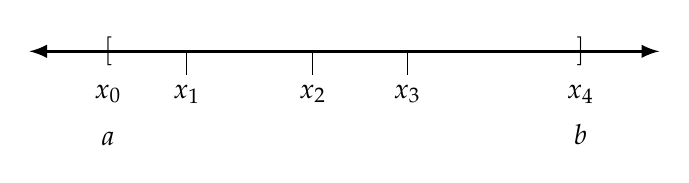
\begin{tikzpicture}[scale=2]
        \draw[very thick, latex-latex] (-2, 0) -- (2, 0);
        \node[] at (-1.5, 0) {$[$};
        \node[below] at (-1.5, -0.15) {$x_0$};
        \node[below] at (-1.5, -0.45) {$a$};
        \node[] at (1.5, 0) {$]$};
        \node[below] at (1.5, -0.15) {$x_4$};
        \node[below] at (1.5, -0.4) {$b$};
        \draw[] (-1, 0) -- (-1, -0.15);
        \node[below] at (-1, -0.15) {$x_1$};
        \draw[] (-0.2, 0) -- (-0.2, -0.15);
        \node[below] at (-0.2, -0.15) {$x_2$};
        \draw[] (0.4, 0) -- (0.4, -0.15);
        \node[below] at (0.4, -0.15) {$x_3$};
    \end{tikzpicture}
    \caption{Visualization of a partition $\set{x_0, x_1, x_2, x_3, x_4}$ of $[a, b]$. Note that the points in the partitions need not be equally spaced.}
    \label{fig27}
\end{figure}

\setcounter{rudin}{0}
\begin{definition}{Upper and Lower Sums}{6.1}
    Given $f: [a, b] \mapsto \RR$ and a partition $P$ of $[a, b]$ let:
    \begin{align*}
        M_i &= \sup\set{f(x): x_{i-1} \leq x \leq x_i}
        \\ m_i &= \inf\set{f(x): x_{i-1} \leq x \leq x_i}
    \end{align*}
    Then, we can define the \textbf{upper} and \textbf{lower sums}:
    \begin{align*}
        U(P, f) &= \sum_{i=1}^n M_i \Delta x_i
        \\ L(P, f) &= \sum_{i=1}^n m_i \Delta x_i
    \end{align*}
\end{definition}

\begin{figure}[htbp]
    \centering
    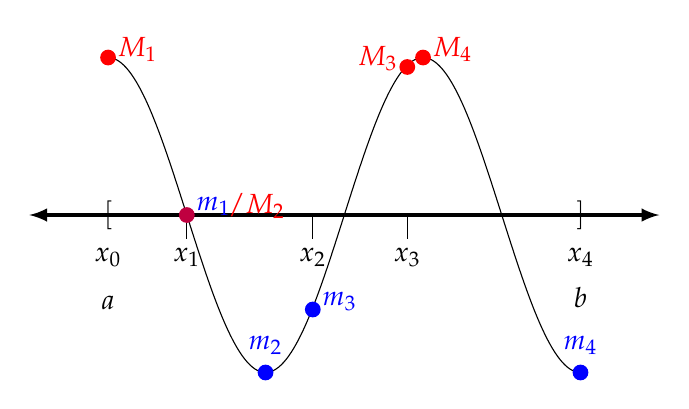
\begin{tikzpicture}[scale=2]
        \draw[very thick, latex-latex] (-2, 0) -- (2, 0);
        \node[] at (-1.5, 0) {$[$};
        \node[below] at (-1.5, -0.15) {$x_0$};
        \node[below] at (-1.5, -0.45) {$a$};
        \node[] at (1.5, 0) {$]$};
        \node[below] at (1.5, -0.15) {$x_4$};
        \node[below] at (1.5, -0.4) {$b$};
        \draw[] (-1, 0) -- (-1, -0.15);
        \node[below] at (-1, -0.15) {$x_1$};
        \draw[] (-0.2, 0) -- (-0.2, -0.15);
        \node[below] at (-0.2, -0.15) {$x_2$};
        \draw[] (0.4, 0) -- (0.4, -0.15);
        \node[below] at (0.4, -0.15) {$x_3$};
        \draw[] (-1, 0) sin (-1.5, 1);
        \draw[] (-1, 0) sin (-0.5, -1);
        \draw[] (0, 0) sin (-0.5, -1);
        \draw[] (0, 0) sin (0.5, 1);
        \draw[] (1, 0) sin (0.5, 1);
        \draw[] (1, 0) sin (1.5, -1);
        \node[circle, fill = red, minimum size = 0.2cm, inner sep = 0pt, label={[right, text=red]:$M_1$}] at (-1.5, 1) {};
        \node[circle, fill = purple, minimum size = 0.2cm, inner sep = 0pt, label={[right, text=blue]:$m_1$}] at (-1, 0) {};
        \node[right, text = red] at (-0.8, 0.06) {$/M_2$};
        \node[circle, fill = blue, minimum size = 0.2cm, inner sep = 0pt, label={[above, text=blue]:$m_2$}] at (-0.5, -1) {};
        \node[circle, fill = blue, minimum size = 0.2cm, inner sep = 0pt, label={[right, text=blue]:$m_3$}] at (-0.2, -0.6) {};
        \node[circle, fill = red, minimum size = 0.2cm, inner sep = 0pt, label={[left, text=red]:$M_3$}] at (0.4, 0.94) {};
        \node[circle, fill = red, minimum size = 0.2cm, inner sep = 0pt, label={[right, text=red]:$M_4$}] at (0.5, 1) {};
        \node[circle, fill = blue, minimum size = 0.2cm, inner sep = 0pt, label={[above, text=blue]:$m_4$}] at (1.5, -1) {};
        \end{tikzpicture}
    \caption{Example of a function $f$, a partition $P$ of $[a, b]$, and the $M_i, m_i$s for this choice of partition.}
    \label{fig28}
\end{figure}

\noindent By construction, it should be evident that $L(P, f) \leq U(P, f)$ for all $P, f$.

A natural question that arises from the form of the above expression is whether these are Riemann sums or not. Recall from first year calculus that we would choose the left endpoint, right endpoint, or some other arbitrary choice of a point in the subinterval. Here, we in a sense use a ``special case'' of the supremum/infimum. We will see that this choice is musch easier to use in proofs due to monotonicity properties. Namely, if we have a partition and add another point, then $U(P, f)$ can only decrease, and $L(P, f)$ can only increase (we will see this in a theorem soon)!


\setcounter{rudin}{0}
\begin{definition}{Upper/Lower Integrals and Riemann Integrability}{6.1}
    We define the \textbf{upper Riemann integral} to be:
    \begin{align*}
        \uint{a}{b} = \inf_P U(P, f).
    \end{align*}
    and the \textbf{lower Riemann integral} to be:
    \begin{align*}
        \lint{a}{b} = \sup_P L(P, f).
    \end{align*}
    Here, the infimum/supremum is taken over all partitions $P$. We say that $f$ is \textbf{Riemann integrable} on $[a, b]$, and write $f \in \R_{[a, b]}$ if:
    \begin{align*}
        \uint{a}{b} = \lint{a}{b}
    \end{align*}
    which we can write as:
    \begin{align*}
        \int_{a}^{b} f dx \text{ or } \int_{a}^{b} f(x) dx
    \end{align*}
\end{definition}
\noindent Note that the choice of variable in the above definition is totally arbitrary. 

Also, note that while $f$ is not required to be continuous in the above definition, it is required to be bounded; else, $M_i$ and $m_i$ may not exist. Since $f$ is bounded, $U(P, f)$, $L(P, f)$ are bounded for all $P, f$ and hence we have a set of real numbers for which we may consider the supremum/infimium of by the LUB/GLB property of the reals. Since the upper/lower sums lie in a bounded interval, there is no questions about whether the lower/upper integrals exist. The question becomes whether they are equal or not. Before getting into further discussion on this topic, we discuss a bound:

\setcounter{rudin}{0}
\begin{theorem}{ML Bounds}{6.1}
    Let $m = \inf\set{f(x): a \leq x \leq b}$ and $M = \sup\set{f(x): a \leq x \leq b}$ (which exist by the boundedness of $f$). Then,
    \begin{align*}
        m(b - a) \leq L(P, f) \leq U(P, f) \leq M(b - a)
    \end{align*}
    For any choice of partition $P$.
\end{theorem}
\begin{nproof}
    For any $i$, we have that:
    \begin{align*}
        m \leq m_i \leq M_i \leq M
    \end{align*}
    Therefore:
    \begin{align*}
        \sum_{i=1}^n m \Delta x_i \leq \sum_{i=1}^n m_i \Delta x_i \leq \sum_{i=1}^n M_i \Delta x_i \leq \sum_{i=1}^n M \Delta x_i
    \end{align*}
    So we conclude that:
    \begin{align*}
        m(b - a) \leq L(P, f) \leq U(P, f) \leq M(b - a)
    \end{align*} \qed
\end{nproof}

\noindent Now that we have established the Riemann integral, a natural question is how can we extend this notion. In order to do so, we will use a montonically increasing function $\alpha: [a, b] \mapsto \RR$ (that is, $\alpha(x) \leq \alpha(y)$ for all $x \leq y$). Note that $\alpha$ need not be continuous. Indeed, compared to the Riemann integral where $\alpha(x) = x$ and was continuous, in this general setting, $\alpha$ is allowed to have jumps. This allows for certain benefits, as we will soon discuss. However, we note that $\alpha$ can only have a finite number of jumps.

\begin{ntheorem}{ 4.30}{}
    Let $\alpha: [a, b] \mapsto \RR$ be monotonic. Then, it can only have finitely many discontinities.
\end{ntheorem}
\begin{nproof}
    Assign a rational number $r(x)$ to each of the discontinuities of $\alpha$. Then, we have that:
    \begin{align*}
        \lim_{x \rightarrow r(x)^-} \alpha(x) < \alpha(x) < \lim_{x \rightarrow r(x)^+} \alpha(x)
    \end{align*}
    Since $x_1 < x_2$ implies $\lim_{x \rightarrow r(x_1)^+} \alpha(x) \leq lim_{x \rightarrow r(x_2)^-} \alpha(x)$, we have that $r(x_1) \neq r(x_2)$ if $x_1 \neq x_2$. We therefore have established a function $r$ from the set of discontinuities of $\alpha$ to the rationals. As the rationals are countable, the set of discontiuities of $\alpha$ are also countable. \qed
\end{nproof}

\noindent With this established, we now define the generalized Riemann-Stieltjes integral.

\begin{definition}{Riemann-Stieltjes Integral}{6.2}
    Let $\alpha: [a, b] \mapsto \RR$ be increasing, and given a partition $P$ of $[a, b]$, define:
    \begin{align*}
        \Delta \alpha_i = \alpha(x_i) - \alpha(x_{i-1}) (\geq 0)
    \end{align*}
    For bounded $f: [a, b] \mapsto \RR$, Let:
    \begin{align*}
        U(P, f, \alpha) &= \sum_{i=1}^n M_i \Delta \alpha_i
        \\ L(P, f, \alpha) &= \sum_{i=1}^n m_i \Delta \alpha_i
    \end{align*}
    We then take the infimum/supremum over partitions $P$ to get:
    \begin{align*}
        \uint{a}{b} f d\alpha &= \inf_P U(P, f, \alpha)
        \\ \lint{a}{b} &= \sup_P L(P, f, \alpha)
    \end{align*}
    If equal, we write their value as:
    \begin{align*}
        \int_a^b f d\alpha \text{ or } \int_a^b f(x)d\alpha(x)
    \end{align*}
    and we write that $f \in \R_{[a, b]}(\alpha)$. In the case where $\alpha(x) = x$, we recover the Riemann integral.
\end{definition}

\noindent Why is this definition useful? What does it accomplish for us that the original Riemann integral does not? We consider a physically motivating example. Suppose we have a thin wire with varying mass density $\rho(x)$. If we wanted to calculate the mass density of the wire, we would integrat the density $\rho(x)$ over the length of the wire. Now, suppose our wire consists of steel of continuously varying mass density, as well as beads/point masses placed on certain locations of the wire. The Riemann integral cannot handle these point masses, but the Riemann-Stieltjes integral can deal with this case if we use an $\alpha$ with discontinuities in it. Hence, the Riemann-Stieltjes integral allows us to handle cases where we both have continuous and discrete masses to integrate over. It acts as a bridge between Riemann and Lebesgue integration (the latter of which will be the subject of a later course in measure theory).

We now will answer the question: ``for what choices of $f, \alpha$ is $f$ Riemann-Stieltjes integrable?''

\subsection{Criterion for Integrability}

\begin{definition}{Refinements and Common Refinemnet}{6.3}
    $P^*$ is a \textbf{refinement} of $P$ if $P \subset P^*$ and $P, P^*$ are partitions. The common refinemnet of $P_1, P_2$ is $P^* = P_1 \cup P_2$.
\end{definition}

\begin{theorem}{}{6.4}
    If $P^*$ is a refinemne tof $P$, then:
    \begin{align*}
        L(P, f, \alpha) \leq L(P^*, f, \alpha) \leq U(P^*, f, \alpha) \leq U(P, f, \alpha)
    \end{align*}
\end{theorem}

\noindent As a remark, when we take infimums/supremums over partitions $P$ to obtain the upper/lower Riemann-Stieltjes integals, we are taking refinements.

Also, note that the above theorem does \textit{not} apply to (right-hand, left-hand, midpoint, arbitrary) Riemann sums, and is a consequence of the choice of upper/lower sums with supremums/infimums taken over the subintervals.

\begin{nproof}
    It suffices to consider $P^*$ with a single extra point $x_{i - 1} < x^* < x_i$, and then the genral case follows by induction.

    For the case where $\alpha(x) = x$, the refinement adds $(m^* - m_i)(x^* - x_{i-1}) \geq 0$. 

    For the general case, we have that:
    \begin{align*}
        L(P^*, f, \alpha) - L(P, f, \alpha) &= \left(m^*(\alpha(x^*) - \alpha(x_{i-1})) + m_i(x^* - x_{i-1}) \right)- m_i(\alpha_{x_i} - \alpha_{x_{i-1}})
        \\ &= \left(m^*(\alpha(x^*) - \alpha(x_{i-1})) + m_i(x^* - x_{i-1}) \right)
        \\ &- m_i\left[(\alpha(x^*) - \alpha(x_{i-1})) + (\alpha(x_i) - \alpha(x^*))\right]
        \\ &= (m^* - m_i)(\alpha(x^*) - \alpha(x_i))
    \end{align*}
    $\alpha$ is montonically increasing, so $x^* \geq x_i$ implies that the second term is positive. Furthermore, $m^* \geq m_i$ as $\inf\set{f(x): x \in [x_{i-1}, x^*]} \geq \inf\set{f(x): x \in [x_{i-1}, x_i]}$. It follows that:
    \begin{align*}
        L(P^*, f, \alpha) - L(P, f, \alpha) \geq 0
    \end{align*} 
    and the proof for $U(P^*, f, \alpha) - U(P, f, \alpha) \leq 0$ follows analogously. \qed
\end{nproof}
\begin{figure}[htbp]
    \centering
    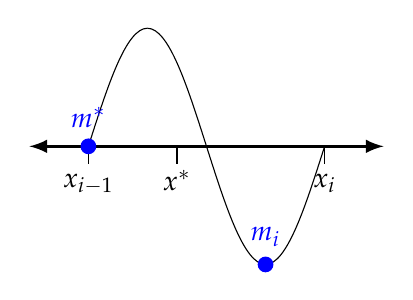
\begin{tikzpicture}[scale=1.5]
        \draw[latex-latex, very thick] (-1.5, 0) -- (1.5, 0);
        \draw[] (-1, 0) sin (-0.5, 1);
        \draw[] (0, 0) sin (-0.5, 1);
        \draw[] (0, 0) sin (0.5, -1);
        \draw[] (1, 0) sin (0.5, -1);
        \draw[] (-1, 0) -- (-1, -0.15);
        \draw[] (1, 0) -- (1, -0.15);
        \node[below] at (-1, -0.15) {$x_{i-1}$};
        \node[below] at (1, -0.15) {$x_i$};
        \draw[] (-0.25, 0) -- (-0.25, -0.15);
        \node[below] at (-0.25, -0.12) {$x^*$};
        %\node[circle, fill = red, minimum size = 0.2cm, inner sep = 0pt, label={[right, text=red]:$M_{i\text{original}}/M_{i\text{new}}$}] at (-0.5, 1) {};
        \node[circle, fill = blue, minimum size = 0.2cm, inner sep = 0pt, label={[above, text=blue]:$m_{i}$}] at (0.5, -1) {};
        %\node[circle, fill = red, minimum size = 0.2cm, inner sep = 0pt, label={[right, text=red]:$M_{i+1\text{new}}$}] at (-0.25, 0.7) {};
        \node[circle, fill = blue, minimum size = 0.2cm, inner sep = 0pt, label={[above, text=blue]:$m^*$}] at (-1, 0) {};
    \end{tikzpicture}
    
    \caption{Visualization of the effect of adding an extra point $x^*$ to the partition $P$. We can see that this has the net effect of increasing $L(P, f, \alpha)$ as $m^* \geq m_i$.}
    \label{fig29}
\end{figure}
\noindent Note that as a point of notation, if $f, \alpha$ are fixed, we sometimes can write $L(P), U(P)$ in place of $L(P, f, \alpha)$ and $U(P, f, \alpha)$. Where $f$ is integrable, we will also sometimes omit the interval and just write $f \in \R(\alpha)$. 

\begin{theorem}{}{6.5}
    $\lint{a}{b} f d\alpha \leq \uint{a}{b} f d\alpha$.
\end{theorem}
\begin{nproof}
    For partitions $P_1, P_2$, let $P^* = P_1 \cup P_2$ be the common refinement. By Theorem \ref{thm:6.4}, we have that:
    \begin{align*}
        L(P_1) \leq L(P^*) \leq U(P^*) \leq U(P_2)
    \end{align*}
    And in particular, $L(P_1) \leq U(P_2)$. Therefore, for any fixed $P_2$, $U(P_2)$ is an upper bound on the set of all lower sums. As the supremum is the least upper bound, we have that:
    \begin{align*}
        \sup_{P_1} L(P_1) \leq U(P_2)
    \end{align*}
    Therefore, as $\sup_{P_1} L(P_1)$ is a lower bound on the set of all upper sums, and the infimum is the greatest lower bound, we have that:
    \begin{align*}
        \sup_{P_1} L(P_1) \leq \inf_{P_2} U(P_2)
    \end{align*}
    So therefore:
    \begin{align*}
        \lint{a}{b} f d\alpha \leq \uint{a}{b} f d\alpha
    \end{align*}
    as claimed. \qed
\end{nproof}

\begin{theorem}{\texorpdfstring{$\e$}{e}-Criterion for Integrability}{6.6}
    $f \in \R(\alpha)$ if and only if for all $\e > 0$, there exists $P_\e$ such that $U(P_\e) - L(P_\e) < \e$. 
\end{theorem}
\begin{nproof}
    $\boxed{\implies}$ By hypothesis, $\sup_P L(P) = \int_a^b fd\alpha = \inf_P U(P)$. Let $\e > 0$. Then by the property of sup/inf, there exist $P_1, P_2$ such that:
    \begin{align*}
        \int_a^b f d\alpha - L(P_1) &< \frac{\e}{2}
        \\ U(P_2) - \int_a^b f d\alpha &< \frac{\e}{2}
    \end{align*}
    Adding the first inequality to the second, we get:
    \begin{align*}
        U(P_2) - L(P_1) < \e
    \end{align*}
    Letting $P^* = P_1\cup P_2$, by Theorem \ref{thm:6.4} we have that:
    \begin{align*}
        U(P^*) - L(P^*) \leq U(P_2) - L(P_1) < \e
    \end{align*}
    which proves the claim.

    $\boxed{\impliedby}$ Let $\e > 0$ Then by Theorem \ref{thm:6.5} we have that:
    \begin{align*}
        0 \leq \uint{a}{b} f d\alpha - \lint{a}{b} f d\alpha
    \end{align*}
    and furthermore:
    \begin{align*}
        0 \leq \uint{a}{b} f d\alpha - \lint{a}{b} f d\alpha \leq U(P_\e) - L(P_\e) < \e
    \end{align*}
    Where the second inequality is true for any choice of partition. $\e$ is arbitrary, so we conclude that:
    \begin{align*}
        \uint{a}{b} f d\alpha - \lint{a}{b} f d\alpha = 0
    \end{align*}
    And therefore $\uint{a}{b} f d\alpha = \lint{a}{b} f d\alpha$, and $f \in \R(\alpha)$. \qed
\end{nproof}

\noindent Theorem 6.7 is a little technical, so we shall skip it for now.

\stepcounter{rudin}
\begin{theorem}{Continuity implies integrability}{6.8}
    If $f$ is continuous on $[a, b]$, then $f \in \R_{[a, b]}(\alpha)$. 
\end{theorem}
\noindent Note in the above theorem that we make no assumptions on $\alpha$, only that (of course) it is monotonic.
\begin{nproof}
    By definition, $U(P) - L(P) = \sum_{i=1}^n (M_i - m_i)\Delta \alpha_i$. The idea will be to choose small intervals to make these differences small. Since $[a, b]$ is compact, $f$ is uniformly continuous by Theorem \ref{thm:4.19}. So, for all $\eta > 0$, there exists $\delta > 0$ such that $\abs{f(x) - f(t)} < \eta$ if $\abs{x - t} < \delta$. Thus, if $P$ is constructed such that $\Delta x_i < \delta$ then $M_i - m_i < \eta$. We then have that:
    \begin{align*}
        U(P) - L(P) \leq \sum_{i=1}^n \eta \Delta \alpha_i = \eta \sum_{i=1}^n (\alpha(x_{i}) - \alpha(x_{i-1})) = \eta\left(\alpha(b) - \alpha(a)\right)
    \end{align*}
    Where in the last equality we use the fact that we have a telescoping sum. Given $\e > 0$, we choose $\eta < \frac{\e}{\alpha(b) - \alpha(a)}$. With this choice of partition with $\Delta x_i < \delta = \delta(\eta)$, we have that:
    \begin{align*}
        U(P) - L(P) < \e
    \end{align*}
    and we conclude that $f \in \R_{[a, b]}(\alpha)$ by Theorem \ref{thm:6.6}. \qed
\end{nproof}
\noindent A natural question is ``what $f$s are Riemann integrable in general?'' The answer turns out to be ``if $f$ is continuous almost everywhere''. This sounds handwavy, but has a precise definition; although it is not covered in this course, one can refer to Rudin 11.33(b) for details. 


\subsection{Properties of the Integral}

\subsection{Integration and Differentiation}


\section[Sequences and Series of Functions]{\hyperlink{toc}{Sequences and Series of Functions}}

\subsection{Motivating Examples}
\begin{nexample}{}{}
    For $m, n \in \NN$, let $p_{n, m} = \frac{m}{n}$. Then, 
    \begin{align*}
        \lim_{m\rightarrow \infty} p_{m, n} = \infty, \quad \linf p_{m, n} = 0
    \end{align*}
    In particular,
    \begin{align*}
        \lim_{m \rightarrow \infty}\linf p_{m, n} = 0, \quad \linf\lim_{m \rightarrow \infty} p_{m, n} = \infty.
    \end{align*}
    Which demonstrates that the order of which limits are taken in can affect the value.
\end{nexample}

\begin{nexample}{}{}
    Define the sequence of functions:
    \begin{align*}
        f_n(x) = \begin{cases}
            1 & x \geq 0
            \\ 1 + nx & -\frac{1}{n} < x < 0
            \\ 0 & x \leq -\frac{1}{n}
        \end{cases}
    \end{align*}
    Since $f_n$ is piecewise linear, it is continuous. However, looking at the $n \rightarrow \infty$ limit, we have:
    \begin{align*}
        \linf f_n(x) = \begin{cases}
            1 & x \geq 0
            \\ 0 & x < 0
        \end{cases}
    \end{align*}
    Which is the right continuous step function, which is evidently discontinuous at $x = 0$. Hence, the limit of continuous functions can be discontinuous. Another way of viewing this problem is:
    \begin{align*}
        \linf \lim_{x \rightarrow 0} f_n(x) = 0, \quad \lim_{x \rightarrow 0} \linf f_n(x) = \text{D.N.E.}
    \end{align*}
    so again we see the order of taking our limits can be important.
\end{nexample}
\begin{figure}[htbp]
    \centering
    \begin{tikzpicture}[scale=1.5]
        \draw[latex-latex, very thick] (-2, 0) -- (2, 0);
        \draw[-latex , very thick] (0, 0) -- (0, 2);
        \draw[<-, thick, blue] (-1.5, 0) -- (-0.5, 0);
        \draw[thick, blue] (-0.5, 0) -- (0, 1);
        \draw[->, thick, blue] (0,1) -- (1.5, 1);
        \draw[] (-0.5, 0) -- (-0.5, -0.15);
        \node[below] at (-0.5, -0.15) {$-\frac{1}{n}$};
    \end{tikzpicture}
    
    
    \caption{Plot of $f_n$ in the above example.}
    \label{fig37}
\end{figure}

\setcounter{rudin}{3}

\begin{example}{}{7.4}
    For $m \in \NN$ and $x \in \RR$, let $f_m(x) = \lim_{n \rightarrow \infty} \left[\cos(m!\pi x)\right]^{2n}$. Since $\abs{\cos(k\pi)} = 1$ if $k \in \ZZ$, we see that $f_m(x) = 1$ when $m! x \in \ZZ$. Conversely, since $\abs{\cos(k\pi)} < 1$ if $k \neq \ZZ$, $f_m(x) = 0$ when $m! x \notin \ZZ$. Some plots of $f_m(x)$ on $[0, 1]$ for $m = 1, 2, 3$ are below as a visualization. We now define $f(x) = \lim_{m \rightarrow \infty} f_m(x)$. If $x = \frac{p}{q} \in \QQ$, then $m! x = \frac{m! p}{q} \in \ZZ$ for $m$ large enough (for $m \geq q$, as the denominator cancells). Therefore, we have that $f(x) = 1$ for $x \in \QQ$. Conversely, if $x \notin \QQ$, then $m! x \notin \ZZ$ for all $m \in \NN$. So, $f_m(x) = 0$ for all $m$, and $f(x) = 0$. Therefore, we have that:
    \begin{align*}
        f(x) = \lim_{m \rightarrow \infty} f_m(x) = \begin{cases}
            1 & x \in \QQ
            \\ 0 & x \notin \QQ
        \end{cases}.
    \end{align*}
    In other words, $f$ is the Dirchlet function. The interesting part is that each of the $f_m(x)$ are Riemann integrable on $[0, 1]$ by Theorem \ref{thm:6.10} (as $f$ has finitely many discontinuities for any $m \in \NN$). However, the limit is not Riemann integrable, as we prove below. Hence, the limit of Riemann integrable functions is not necessarily Riemann integrable.
\end{example}

\begin{figure}[htbp]
    \centering
    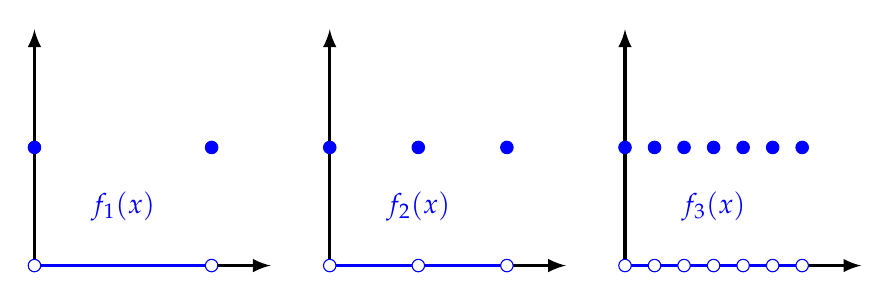
\begin{tikzpicture}[scale = 1.5]
        \draw[-latex, very thick] (0, 0) -- (0, 2);
        \draw[-latex, very thick] (0, 0) -- (2, 0);
        \draw[-latex, very thick] (2.5, 0) -- (2.5, 2);
        \draw[-latex, very thick] (2.5, 0) -- (4.5, 0);
        \draw[-latex, very thick] (5, 0) -- (5, 2);
        \draw[-latex, very thick] (5, 0) -- (7, 0);
        \filldraw[blue] (0, 1) circle (1.5pt);
        \filldraw[blue] (1.5, 1) circle (1.5pt);
        \draw[thick, blue] (0, 0) -- (1.5, 0);
        \draw[blue, fill = white] (0, 0) circle (1.5pt);
        \draw[blue, fill = white] (1.5, 0) circle (1.5pt);
        \node[text = blue] at (0.75, 0.5) {$f_1(x)$};

        \filldraw[blue] (2.5, 1) circle (1.5pt);
        \filldraw[blue] (3.25, 1) circle (1.5pt);
        \filldraw[blue] (4, 1) circle (1.5pt);
        \draw[thick, blue] (2.5, 0) -- (4, 0);
        \draw[blue, fill = white] (2.5, 0) circle (1.5pt);
        \draw[blue, fill = white] (3.25, 0) circle (1.5pt);
        \draw[blue, fill = white] (4, 0) circle (1.5pt);
        \node[text = blue] at (3.25, 0.5) {$f_2(x)$};

        \filldraw[blue] (5, 1) circle (1.5pt);
        \filldraw[blue] (5.25, 1) circle (1.5pt);
        \filldraw[blue] (5.5, 1) circle (1.5pt);
        \filldraw[blue] (5.75, 1) circle (1.5pt);
        \filldraw[blue] (6, 1) circle (1.5pt);
        \filldraw[blue] (6.25, 1) circle (1.5pt);
        \filldraw[blue] (6.5, 1) circle (1.5pt);
        \draw[thick, blue] (5, 0) -- (6.5, 0);
        \draw[blue, fill = white] (5, 0) circle (1.5pt);
        \draw[blue, fill = white] (5.25, 0) circle (1.5pt);
        \draw[blue, fill = white] (5.5, 0) circle (1.5pt);
        \draw[blue, fill = white] (5.75, 0) circle (1.5pt);
        \draw[blue, fill = white] (6, 0) circle (1.5pt);
        \draw[blue, fill = white] (6.25, 0) circle (1.5pt);
        \draw[blue, fill = white] (6.5, 0) circle (1.5pt);
        \node[text = blue] at (5.75, 0.5) {$f_3(x)$};
    \end{tikzpicture}
    \caption{Plot of $f_m(x)$ over the interval $[0, 1]$ for $m = 1, 2, 3$. For $m = 1$, only $x = 0, 1$ satisfy $m! x = x \in \ZZ$. For $m = 2$, we have that $x = 0, \frac{1}{2}, 1$ satisfy $m!x = 2x \in \ZZ$. Finally, for $m = 3$, we have that $x = 0, \frac{1}{6}, \frac{2}{6}, \frac{3}{6}, \frac{4}{6}, \frac{5}{6}, 1$ satisfy $m!x = 6x \in \ZZ$.}
    \label{fig38}
\end{figure}

\noindent We now show that $f$ defined in the above example is not Riemann integrable on $[0, 1]$.

\begin{proof}
    Consider any partition $P$ of $[0, 1]$. Due to the density of rational and irrational numbers in $\RR$ (Theorem \ref{thm:1.20}) we have that $M_i = \sup{f(x): x \in [x_{i-1}, x_i]} = 1$ and $m_i = \inf{f(x): x \in [x_{i-1}, x_i]} = 0$ for all $i$. Therefore, we have that $U(P, f) = \sum_{i=1}^N M_i \Delta x_i = 1$ and $L(P, f) = \sum_{i=1}^N m_i \Delta x_i = 0$ for all partitions $P$. Therefore, $\sup_P U(P, f) = 1$ and $\inf_P L(P, f) = 0$, and we conclude that $f$ is not Riemann integrable on $[0, 1]$.
\end{proof}


\begin{nexample}{}{}
    Define $f_n$ such that:
    \begin{align*}
        f_n(x) = \begin{cases}
            0 & \abs{x} \geq \frac{1}{n}
            \\ n(nx+1) & -\frac{1}{n} < x < 0
            \\ -n(nx+1) & 0 < x < \frac{1}{n}
            \\ 0 & x = 0
        \end{cases}
    \end{align*}
    Then, we have that $f(x) = \linf f_n(x) = 0$ for all $x$.  Furthermore, we have that $\int_{-1}^1 f_n(x)dx = 1$ for all $n$, but $\int_{-1}^1 f(x)dx = 0$. Hence, we have that:
    \begin{align*}
        \linf \int_{-1}^1 f_n(x)dx = 1 \neq 0 = \int_{-1}^1 \linf f_n(x) dx
    \end{align*}
    showing that problems can arise when we interchange the order of an integral with a limit.
\end{nexample}

\begin{figure}[htbp]
    \centering
    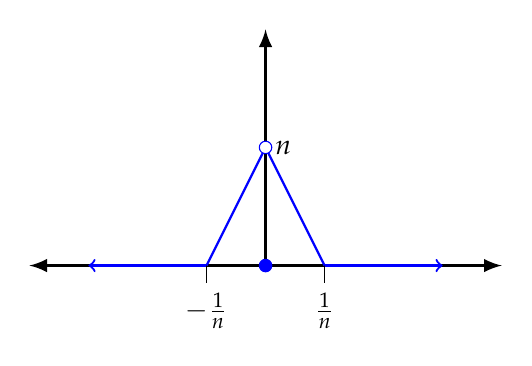
\begin{tikzpicture}[scale=1.5]
        \draw[latex-latex, very thick] (-2, 0) -- (2, 0);
        \draw[-latex , very thick] (0, 0) -- (0, 2);
        \draw[<-, thick, blue] (-1.5, 0) -- (-0.5, 0);
        \draw[thick, blue] (-0.5, 0) -- (0, 1);
        \draw[thick, blue] (0, 1) -- (0.5, 0);
        \draw[->, thick, blue] (0.5, 0) -- (1.5, 0);
        \filldraw[blue] (0, 0) circle (1.5pt);
        \draw[blue, fill = white] (0, 1) circle (1.5pt);
        \node[right] at (0, 1) {$n$};
        \draw[] (-0.5, 0) -- (-0.5, -0.15);
        \node[below] at (-0.5, -0.15) {$-\frac{1}{n}$};
        \draw[] (0.5, 0) -- (0.5, -0.15);
        \node[below] at (0.5, -0.15) {$\frac{1}{n}$};
    \end{tikzpicture}
    
    \caption{Plot of $f_n$ in the above example.}
    \label{fig39}
\end{figure}

\begin{example}{}{7.5}
    Let $f_n(x) = \frac{\sin nx}{\sqrt{n}}$ for $n \in \NN, x \in \RR$. Then, let $f(x) = \linf f_n(x) = 0$ for all $x \in \RR$, so $f'(x) = 0$. However, $f'_n(x) = \frac{1}{\sqrt{n}}n \cos n x = \sqrt{n} \cos n x$ and $\linf \sqrt{n} \cos n x$ does not exist. For example, $f_n'(\pi) = \sqrt{n}(-1)^n$ which is a divergent sequence. So:
    \begin{align*}
        f'(\pi) = \left(\linf f_n\right)'(\pi) = 0 \neq \linf f_n'(\pi)
    \end{align*}
    whcih shows us that problems can arise when interchanging a derivative (which is just a type of limit) with a limit.
\end{example}
\noindent With the above five examples, we have seen examples of bad behaviour that can occur under interchange of limits. Namely:
\begin{enumerate}[1.]
    \item An interchange of the order of limits can change the limiting value for a double sequence.
    \item The limit of a sequence of continuous functions is not necessarily continuous.
    \item The limit of a sequence of Riemann integrable functions is not necessarily Riemann integrable.
    \item The limit of a sequence of Riemann integrals can differ from the Riemann integral of the limit of a sequence.
    \item The limit of a sequence of derivatives can differ from the derivative of a limit of a sequence.
\end{enumerate}

\noindent The good news is that in all of these examples, the sequences we looked at had a ``weak'' form of convergence, where we fix $x$ and then take the $n \rightarrow \infty$ limit. We will now proceed to look at a stronger version of convergence, which looks at ``all $x$ at once'', ensuring that this bad behaviour does not (for the most part) occur.

\subsection{Uniform Convergence}

\setcounter{rudin}{6}
\begin{definition}{Uniform Convergence}{7.7}
    
\end{definition}

\begin{nexample}{}{}
    
\end{nexample}

\begin{nexample}{}{}
    
\end{nexample}

\begin{theorem}{Cauchy Criterion for Uniform Convergence}{7.8}
    
\end{theorem}
\begin{nproof}
    
\end{nproof}

\begin{theorem}{}{7.9}
    
\end{theorem}
\begin{nproof}
    
\end{nproof}

\begin{ndef}{: Uniform Convergence of Series}{}
    
\end{ndef}

\begin{theorem}{Weierstrauss M-Test}{7.10}
    
\end{theorem}
\begin{nproof}
    
\end{nproof}

\subsection{Uniform Convergence and Integration}

\subsection{Uniform Convergence and Differentiation}

\subsection{Equicontinuituous Families of Functions}

\subsection{The Stone-Weierstrauss Theorem}


\section[Some Special Functions]{\hyperlink{toc}{Some Special Functions}}

\subsection{Power Series, Revisited}
Recall our definition of power series (Definition \ref{def:3.38}), functions of the form:
\begin{align*}
    f(x) = \sum_{n=0}^\infty c_n x^n.
\end{align*}
Also recall the radius of convergence (Theorem \ref{thm:3.39}) of such power series, defined as:
\begin{align*}
    R = \frac{1}{\limsup_{n \rightarrow \infty}\sqrt[n]{\abs{c_n}}}.
\end{align*}
Note that if $\limsup_{n \rightarrow \infty}\sqrt[n]{\abs{c_n}} = \infty$, then $R = 0$, and if $\limsup_{n \rightarrow \infty}\sqrt[n]{\abs{c_n}} = 0$, then $R = \infty$. The series converges absolutely for $\abs{x} < R$ and diverges for $\abs{x} > R$.

\begin{figure}[htbp]
    \centering
    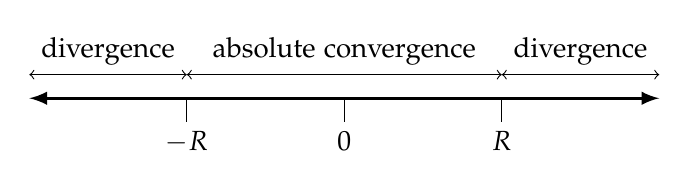
\begin{tikzpicture}[scale=2]
        \draw[latex-latex, very thick] (-2, 0) -- (2, 0);
        \draw[] (0, 0) -- (0, -0.15);
        \draw[] (1, 0) -- (1, -0.15);
        \draw[] (-1, 0) -- (-1, -0.15);
        \node[below] at (0, -0.15) {$0$};
        \node[below] at (1, -0.15) {$R$};
        \node[below] at (-1, -0.15) {$-R$};
        \draw[<->] (1, 0.15) -- (-1, 0.15);
        \draw[<->] (1, 0.15) -- (2, 0.15);
        \draw[<->] (-1, 0.15) -- (-2, 0.15);
        \node[above] at (0, 0.15) {absolute convergence};
        \node[above] at (1.5, 0.15) {divergence};
        \node[above] at (-1.5, 0.15) {divergence};
    \end{tikzpicture}
    
    \caption{Visualization of the radius of convergence for $f(x) = \sum_{n=0}^\infty c_nx^n$, $x \in \RR$.}
    \label{fig49}
\end{figure}

\begin{theorem}{}{8.1}
    If $\sum_{n=0}^\infty c_nx^n$ converges for $\abs{x} < R$, let $f(x) = \sum_{n=0}^\infty c_n x^n$ for $\abs{x} < R$. Then, the series converges uniformly on $[-R + \e, R - \e]$ for any $\e > 0$, $f$ is differentiable (and hence continuous) on $(-R, R)$ and $f'(x) = \sum_{n=0}^\infty nc_nx^{n-1}$. 
\end{theorem}

\begin{nproof}
    We first show the uniform convergence on $[-R + \e, R - \e]$. For $\abs{x} \leq R - \e$, we have that $\abs{c_nx^n} \leq \abs{x_n}(R - \e)^n$. Since $\sum_n \abs{c_n}(R - \e)^n < \infty$ (by the assumed absolute convergence on $(-R, R)$), we have that $\sum_n c_nx^n$ converges uniformly in $\abs{x} \leq R - \e$ by the M-test (Theorem \ref{thm:7.10}).

    We next prove the claim about the differentiability/derivative of $f$. The radius of convergence of $\sum_n nc_n x^{n-1}$ is:
    \begin{align*}
        \frac{1}{\limsup_{n \rightarrow \infty}\sqrt[n]{\abs{nc_n}}} = \frac{1}{\limsup_{n \rightarrow \infty}\sqrt[n]{\abs{c_n}}} = R
    \end{align*}
    so since $f$ converges in $(-R, R)$, so does $\sum_n nc_nx^{n-1}$. Now, let $s_n(x) = \sum_{m=0}^n c_mx^m$. Then, by the linearity of the derivative we have that $s_n'(x) = \sum_{m=1}^n mc_mx^{m-1}$. By the first part of the proof, we have that $s_n'(x) \rightarrow \sum_{m=1}^\infty mc_mx^{m-1}$ uniformly on $[-R + \e, R - \e]$. Since $s_n(x) \rightarrow f(x)$ uniformly, by Theorem \ref{thm:7.17}, we have that $f'$ exists on $[-R +\e, R - \e]$ and $f'(x) = \sum_{m=1}^\infty mc_mx^{m-1}$. Since $\e$ is arbitrary, $f'$ exists and is equal to $\sum_{m=1}^\infty mc_mx^{m-1}$ for all $x \in (-R, R)$. \qed 
\end{nproof}
\noindent As a remark, note that we can (interestingly) prove the differentiability of $f$ on $(-R, R)$ from the uniform convergence on $[-R + \e, R - \e]$.

\begin{ncorollary}{}{}
    If $f(x) = \sum_{n=0}^\infty c_nx^n$ converges for $\abs{x} < R$, then $f^{(k)}(x)$ exists for all $k \in \NN$ and for all $x \in (-R, R)$. It is given by:
    \begin{align*}
        f^{(k)}(x) = \sum_{n=k}^\infty n(n-1)\ldots(n-k+1)c_nx^{n-k} \quad (*)
    \end{align*}
    and consequently, we have that $c_k = \frac{f^{(k)(0)}}{k!}$, so $f(x) = \sum_{n=0}^\infty \frac{f^{(n)}(0)}{n!}x^n$.
\end{ncorollary}
\noindent Compare the above Corollary to Taylor's theorem (Theorem \ref{thm:5.15}). Here, we take our taylor polynomial and extend it to an infinite series (the limit of polynomials). 

\begin{nproof}
    By Theorem \ref{thm:8.1}, we have that $f'(x) = \sum_{n=1}^\infty nc_nx^{n-1}$ and $f''(x) = \sum_{n=2}^\infty n(n-1)c_nx^{n-2}$ and so on. Setting $x = 0$ in $(*)$, we have that $f^{(k)}(0) = n(n-1)\ldots 1 c_n = n! c_k$, so $c_n = \frac{f^{(k)}(0)}{n!}$. \qed
\end{nproof}
\noindent Recall the definition of \emph{analytic functions}, which are infinite differentiable and can be represented as sums or series of derivatives evaluated at zero. 

\begin{nexample}{}{}
    As we discussed in Chapter 5, there are infinitely differentiable functions that are not analytic. Let:
    \begin{align*}
        f(x) = \begin{cases}
            \exp(-\frac{1}{x^2}) & x \neq 0
            \\ 0 & x = 0
        \end{cases}
    \end{align*}
    By Theorem \ref{thm:8.1}, $f$ is infinitely differentiable, and $f^{(n)}(0) = 0$ for all $n \in \NN$. But, $f(x) \neq 0$ except at $x = 0$. Hence, $f(x) \neq \sum_{n=0}^\infty \frac{f^{(n)}(0)}{n!}x^n$ except at $x = 0$. This is true despite the fact that the RHS converges to zero for all $x \in \RR$. 
\end{nexample}

\begin{nexample}{}{}
    Bump functions are continuous, infinitely differentiable functions of compact support (it is zero outside of a compact set). For example, 
    \begin{align*}
        f(x) = \begin{cases}
            \exp(-\frac{1}{1-x^2}) & x \in (-1, 1)
            \\ 0 & \abs{x} \geq 1
        \end{cases}
    \end{align*}
    is an example of a bump function. Such functions are very useful in the study of functional analysis and PDEs.
\end{nexample}
\begin{figure}[htbp]
    \centering
    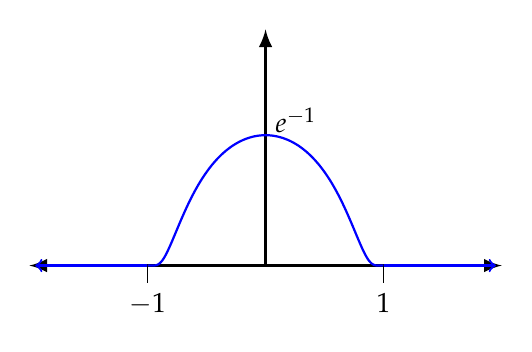
\begin{tikzpicture}[scale=1.5]
        \draw[-latex, very thick] (0, 0) -- (0, 2);
        \draw[latex-latex, very thick] (-2, 0) -- (2, 0);
        \draw[blue, thick, smooth, samples = 100, domain=-0.999:0.999, variable = \x] plot(\x, {3*exp(-1/(1-(\x)*(\x)))});
        \draw[->, blue, thick] (1, 0) -- (1.95, 0);
        \draw[->, blue, thick] (-1, 0) -- (-1.95, 0);
        \draw[] (1, 0) -- (1, -0.15);
        \draw[] (-1, 0) -- (-1, -0.15);
        \node[below] at (1, -0.15) {$1$};
        \node[below] at (-1, -0.15) {$-1$};
        \node[right] at (0, 1.23) {$e^{-1}$};
    \end{tikzpicture}
    
    \caption{Plot of the bump function $f$ from the above example.}
    \label{fig50}
\end{figure}

\noindent Before we continue, some remarks on the radius of convergence are in order. Of course, the definition of $R = \frac{1}{\limsup_{n \rightarrow \infty}\sqrt[n]{\abs{c_n}}}$ always holds. But in practice, the ratio test is much nicer to use (though it does not always work). We can make the observation that:
\begin{align*}
    \abs{\frac{c_{n+1}x^{n+1}}{c_nx^n}} = \abs{x}\abs{\frac{c_{n+1}}{c_n}} \rightarrow \abs{x}L
\end{align*}
Where we take the $n \rightarrow \infty$ limit in the final expression (assuming the limit exists). We have that the power series converges if $\abs{x} < \frac{1}{L}$ and diverges if $\abs{x} > \frac{1}{L}$. So, when the limit exists, we can write:
\begin{align*}
    R = \frac{1}{\linf\abs{\frac{c_{n+1}}{c_n}}}.
\end{align*}
In general, by Theorem 3.37 (not covered in lecture in 320, see Rudin), we have that:
\begin{align*}
    \frac{1}{\limsup_{n \rightarrow \infty}\abs{\frac{c_{n+1}}{c_n}}} \leq R \leq \frac{1}{\liminf_{n \rightarrow \infty}\abs{\frac{c_{n+1}}{c_n}}}
\end{align*}

\begin{theorem}{Abel's Theorem}{8.2}
    Suppose $\sum_{n=0}^\infty c_n$ converges (perhaps conditionally). Let $f(x) = \sum_{n=0}^\infty c_nx^n$. Then, $f(x)$ converges if $\abs{x} < 1$, and $\lim_{x \rightarrow 1^{-}}f(x) = \sum_{n=0}^\infty c_n$. 
\end{theorem}
\begin{nproof}
    For the first claim, we have that $\limsup_{n \rightarrow \infty}\sqrt[n]{\abs{c_n}} \leq 1$ so by the root test, $\sum_n c_n x^n$ has $R \geq 1$. The interesting case is when $R = 1$ (as if $R > 1$, then $f$ is continuous on $(-R, R)$ and the result follows immediately). In this case, $f(x)$ converges if $\abs{x} < 1$. Let $s_n = \sum_{m=0}^n c_m$ and $s = \sum_{m=0}^\infty c_m = \lim_{n \rightarrow \infty}s_n$. Let $s_{-1} = 0$. Then, we have that $s_n - s_{n-1} = c_n$ for $n \geq 0$.

    Let $\e > 0$. We wish to show that there exists $\delta > 0$ such that for $1 -\delta < x < 1$ we have that $\abs{f(x) - s} < \e$. We start with the partial sum of $f(x)$. For $\abs{x} < 1$, we have:
    \begin{align*}
        \sum_{m=0}^n c_mx^m &= \sum_{m=0}^n (s_m - s_{m-1})x^m
        \\ &= \sum_{m=0}^n s_mx^m - x\sum_{m=0}^{n-1}s_m x^m
        \\ &= (1-x)\sum_{m=0}^n s_mx^m + s_nx^{n+1}.
    \end{align*}
    Now, let $n \rightarrow \infty$. We then have that $s_nx^{n+1} \rightarrow 0$ as $s_n \rightarrow s$ and $x^{n+1} \rightarrow 0$. We then have that $f(x) = (1-x)\sum_{m=0}^n s_mx^m + 0$, and using that $\sum_{m=0}^\infty x^m = \frac{1}{1-x}$, we obtain that:
    \begin{align*}
        \abs{f(x) - s} = \abs{(1-x)\sum_{m=0}^\infty(s_m - s)x^m} \leq \abs{1 - x}\sum_{m=0}^\infty \abs{s_m - s}\abs{x}^m.
    \end{align*}
    Now, choose $N$ such that $m \geq N$ implies $\abs{s_m - s} < \frac{\e}{2}$. Let $x \in (0, 1)$, and then:
    \begin{align*}
        \abs{f(x) - s} \leq (1-x)\sum_{m=0}^N\abs{s_m - s}x^n + (1-x)\frac{\e}{2}\frac{1}{1-x}
    \end{align*}
    The second term on the RHS is bounded using the geometric series. The first term is a polyonimal in $x$ and hence continuous everywhere (including at $x = 1$). It equals $0$ at $x = 1$, so it has absolute value less than $\frac{\e}{2}$ if $x \in (1-\delta, 1)$ for some $\delta$. Hence:
    \begin{align*}
        \abs{f(x) - s} < \frac{\e}{2} + \frac{\e}{2} = \e
    \end{align*}
    \noindent See Rudin page 175 for an application of this Theorem to prove Theorem 3.51 in a different way. Not that for the case where $\sum_n c_n = \infty$, the theorem still holds, with $\lim_{x \rightarrow 1^-}\sum_{n=0}^\infty c_nx^n = \infty$. \qed
\end{nproof}

\begin{theorem}{}{8.3}
    Suppose $\sum_{i=1}^\infty \left(\sum_{j=1}^\infty \abs{a_{ij}}\right) < \infty$. Then, $\sum_{i=0}^\infty \sum_{j=0}^\infty a_{ij} = \sum_{j=0}^\infty \sum_{i=0}^\infty a_{ij}$ (and both converge).
\end{theorem}
\begin{nproof}
    Rudin uses an overly clever proof. See HW7Q2 for a more natural one. \qed
\end{nproof}

\begin{theorem}{}{8.4}
    Suppose $f(x) = \sum_{n=0}^\infty c_nx^n$ has radius of convergence $R$ (Taylor series of $f$ at 0/Maclaurin series). Let $\abs{a} < R$. Then, $f(x) = \sum_{n=0}^\infty \frac{f^{(n)}(0)}{n!}(x-a)^n$ for (at least) $\abs{x - a} < R - \abs{a}$. 
\end{theorem}
\begin{figure}[htbp]
    \centering
    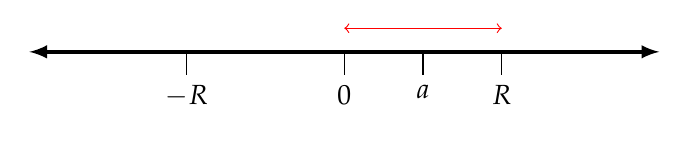
\begin{tikzpicture}[scale=2]
        \draw[latex-latex, very thick] (-2, 0) -- (2, 0);
        \draw[] (0, 0) -- (0, -0.15);
        \draw[] (1, 0) -- (1, -0.15);
        \draw[] (-1, 0) -- (-1, -0.15);
        \draw[] (0.5, 0) -- (0.5, -0.15);
        \node[below] at (0, -0.15) {$0$};
        \node[below] at (1, -0.15) {$R$};
        \node[below] at (-1, -0.15) {$-R$};
        \node[below] at (0.5, -0.15) {$a$};
        \draw[<->, red] (1, 0.15) -- (0, 0.15);
    \end{tikzpicture}
    
    \caption{Visualization of Theorem \ref{thm:8.4}. The new Taylor series around $x = a$ converges in the region up to the radius of convergence of the original series.}
    \label{fig51}
\end{figure}

\begin{nproof}
    We have that $f(x) = \sum_{n=0}^\infty c_n\left[(x - a) + a\right]^n = \sum_{n=0}^\infty c_n\sum_{m=0}^n \binom{n}{m}(x-a)^ma^{n-m}$, and we want to find a way to interchange the order of summation. By Theorem \ref{thm:8.3}, the interchange is permitted if:
    \begin{align*}
        \sum_{n=0}^\infty\sum_{m=0}^n \abs{c_n}\binom{n}{m}\abs{x-a}^m\abs{a}^{n-m} < \infty
    \end{align*}
    but the above is equaivalent to:
    \begin{align*}
        \sum_{n=0}^\infty \abs{c_n}\left(\abs{x - a} + \abs{a}\right)^n
    \end{align*}
    which converges if $\abs{x - a} + \abs{a} < R$. Therefore:
    \begin{align*}
        f(x) = \sum_{m=0}^\infty \sum_{n=m}^\infty c_n\binom{n}{m}a^{n-m}(x - a)^m
    \end{align*}
    over $n \geq m$. We need to show that these new coefficients $\left(\sum_{n=m}^\infty c_n\binom{n}{m}a^{n-m}\right)$ are equal to $\frac{f^{(m)}(a)}{m!}$. Expanding out, we have that:
    \begin{align*}
        \sum_{n=m}^\infty c_n\binom{n}{m}a^{n-m} = \frac{1}{m!}n(n-1)\ldots (n-m+1)c_na^{n-m} = \frac{1}{m!}f^{(m)}(a)
    \end{align*}
    where in the last equality we use Theorem \ref{thm:8.1}. We conclude that:
    \begin{align*}
        f(x) = \sum_{m=0}\frac{f^{(m)}(a)}{m!}(x-a)^m \text{ for } \abs{x - a} < R - \abs{a}
    \end{align*}
\end{nproof}

\begin{nexample}{}{}
    Let $f(x) = \sum_{n=0}^\infty x^n$. If $\abs{x} < 1$, then the series converges and $f(x) = \frac{1}{1-x}$ ($R = 1$). Choose $a = -\frac{1}{2}$ (we look at the Taylor serires around $x = -\frac{1}{2}$). For any $\abs{x} < 1$, we have that $f^{(n)}(x) = \frac{n!}{(1-x)^{n+1}}$, so therefore:
    \begin{align*}
        f^{(n)}(-\frac{1}{2}) = \frac{n!}{(1+\frac{1}{2})^{n+1}} = \left(\frac{2}{3}\right)^{n+1}n!.
    \end{align*}
    By Theorem \ref{thm:8.4}, we then have that:
    \begin{align*}
        f(x) = \sum_{n=0}^\infty \frac{\left(\frac{2}{3}\right)^{n+1}n!}{n!}(x - a)^n = \sum_{n=0}^\infty \left(\frac{2}{3}\right)^{n+1}(x + \frac{1}{2})^n
    \end{align*}
    which is valid for $\abs{x - (-\frac{1}{2})} < 1 - \abs{-\frac{1}{2}}$ and hence if $\abs{x + \frac{1}{2}} < \frac{1}{2}$. Note that in fact, $\sum_{n=0}^\infty\left(\frac{2}{3}\right)^{n+1}(x - a)^n$ converges whenever $\abs{\frac{2}{3}(x + \frac{1}{2})} < 1$, in other words, whenever $\abs{x + \frac{1}{2}} < \frac{3}{2}$, so the series converges in $(-\frac{3}{2}, \frac{1}{2})$. 
\end{nexample}
\begin{figure}[htbp]
    \centering
    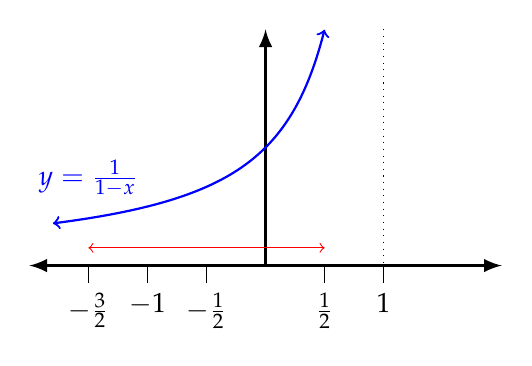
\begin{tikzpicture}[scale=1.5]
        \draw[-latex, very thick] (0, 0) -- (0, 2);
        \draw[latex-latex, very thick] (-2, 0) -- (2, 0);
        \draw[blue, thick, smooth, <->, samples = 100, domain=-1.8:0.5, variable = \x] plot(\x, {1/(1 - (\x))});
        \draw[] (1, 0) -- (1, -0.15);
        \draw[] (-1, 0) -- (-1, -0.15);
        \draw[] (-0.5, 0) -- (-0.5, -0.15);
        \draw[] (-1.5, 0) -- (-1.5, -0.15);
        \draw[] (0.5, 0) -- (0.5, -0.15);
        \node[below] at (0.5, -0.15) {$\frac{1}{2}$};
        \node[below] at (1, -0.15) {$1$};
        \node[below] at (-1, -0.15) {$-1$};
        \node[below] at (-0.5, -0.15) {$-\frac{1}{2}$};
        \node[below] at (-1.5, -0.15) {$-\frac{3}{2}$};
        \node[above, text = blue] at (-1.5, 0.5) {$y = \frac{1}{1-x}$};
        \draw[dotted] (1, 2) -- (1, -0.15);
        \draw[<->, red] (-1.5, 0.15) -- (0.5, 0.15);
    \end{tikzpicture}
    
    \caption{Plot of $y = \frac{1}{1-x}$ and region for which the Taylor series around $a = -\frac{1}{2}$ is valid (red).}
    \label{fig52}
\end{figure}
\noindent As a remark, note that although Theorem \ref{thm:8.4} only guarantees convergence up to the previous boundary, in general the Taylor series will converge up to the nearest singularity. The above theorem is a good example of \emph{analytic continuation}, where a representation of a function converges in a larger interval than the original series (notice that the above taylor series for $f$ around $a = -\frac{1}{2}$ converges up to $-\frac{3}{2}$, when the original series only converged up to $-1$). We extend the function to a larger interval.

Note that there is another way to obtain the Taylor series around $a = -\frac{1}{2}$ (in a technique reminiscent of that used in MATH 300). We can cleverly manipulate the original expression and the geometric series formula to observe that:
\begin{align*}
    f(x) = \frac{1}{1 - x} = \frac{1}{1 - x + \frac{1}{2} - \frac{1}{2}} = \frac{2}{3}\frac{1}{1 - \frac{2}{3}(x + \frac{1}{2})} = \frac{2}{3}\sum_{n=0}^\infty \left(\frac{2}{3}\right)^n (x + \frac{1}{2})^n.
\end{align*}

\begin{theorem}{Principle of Permanence of Form}{8.5}
    Suppose $\sum_n a_n x^n$ and $\sum_n b_n x^n$ each have radius of convergence larger or equal to $R$. Suppose $D \subset (-R, R)$ has a limit point in $(-R, R)$ (for example, $D = \set{\frac{R}{n}: n = 2, 3, \ldots}$ with limit point $0$). If $\sum_n a_nx^n = \sum_n b_n x^n$ in all $x \in D$, then $a_n = b_n$ for all $n \in \NN$ and $\sum_n a_nx^n$ and $\sum_n b_n x^n$ for all $x \in (-R, R)$. 
\end{theorem}
\noindent Note that this also holds for complex variables, so it can be a way of taking things we know in a real context and promoting it to a complex context. We will first prove a lemma.

\begin{nlemma}{ (Problem 2.6)}{}
    Let $E \subset X$ for a metric space $X$. Then the set $E'$ of limit points of $E$ is closed.
\end{nlemma}
\begin{nproof}
    Let $x$ be a limit point of $E'$. We wish to show that $x \in E'$. Let $\delta > 0$. Since $x$ is a limit point of $E'$, for any $r > 0$ there exists some $y \in E'$, $y \neq x$ such that $y \in N_r(x)$. Since $y \in E'$, for any $\delta - r > 0$ we have that $N_{\delta-r}(y)$ contains a point $z$ of $E$. Therefore, we have that:
    \begin{align*}
        d(x, z) \leq d(x, y) + d(y, z) < r + \delta - r = \delta
    \end{align*}
    so any neighbourhood $N_\delta(x)$ of $x$ contains some point of $E$. Hence, $x$ is a limit point of $E$ and $x \in E'$. Hence $E'$ is closed. \qed
\end{nproof}
\noindent We now move to the proof of the theorem.
\begin{nproof}
    Let $c_n = a_n - b_n$ and $f(x) = \sum_n c_nx^n$. Then, $f(x) = 0$ for all $x \in D$. Let $E = \set{x \in (-R, R): f(x) = 0}$, so $D \subset E$. We want to show that $E = (-R, R)$. Let $A = E' \cap (-R, R)$. By hypothesis, $A \neq \emptyset$ as $D$ has a limit point in $(-R, R)$. Let $B = (-R, R) \setminus A$. Then, $(-R, R) = A \cup B$ and $A \cap B = \emptyset$. By the above Lemma, the set of limit points $E'$ is closed. Hence, $A$ is closed and $B$ is open. We claim that $A$ is also open.

    To see that this is the case, we show that $E'$ is open (then $E' \cap (-R, R)$ is open as a finite intersection of open sets is open). Let $x_0 \in A$. Then, there exists $d_n$ such that $f(x) = \sum_n d_n(x - x_0)^n$ for $\abs{x - x_0} < R - \abs{x_0}$ by Theorem \ref{thm:8.4}. We will show that $d_n = 0$ for all $n$, showing that $f(x) = 0$ for all $x \in I_0 = N_{R - \abs{x_0}}(x_0)$, and therefore that $A$ is open. Suppose for the sake of contradiction that this is false. Then, there exists $k$ such that $d_k \neq 0$, i.e. $f(x) = \sum_{n=k}^\infty d_n(x - x_0)^n$ with $d_k \neq 0$. So, $f(x) = (x-x_0)^k\sum_{n=0}^\infty d_{n+k}(x - x_0)^n = g(x)$. Then, $g(x_0) = d_k \neq 0$. By the continuity of $g$, there exists $\delta > 0$ such that $g(x) \neq 0$ for $\abs{x - x_0} < \delta$. But then, $f(x) = (x - x_0)^kg(x) \neq 0$ if $0 < \abs{x - x_0} < \delta$. But then we have that there exists a neighbourhood of $x_0$ such that $f(x) \neq 0$, but then $x_0$ cannot be a limit point of $\set{x: f(x) = 0}$. So, $x_0 \notin A$, which is a contradiction. Hence $d_n = 0$ for all $n \in \NN$, and $A$ is open. 
    
    Given the claim, we have that $A \cap \overline{B} = \overline{A} \cap B = \emptyset$ and hence $A$ and $B$ are separated sets. Since $(-R, R)$ is connected and equals $A \cup B$, one of $A, B$ must be empty. It cannot be $A$ (as $E' \neq \emptyset$ by assumption) so it must be $B$. Hence $B = \emptyset$ and $A = (-R, R) = E'$. This means that any $x \in (-R, R)$ is a limit point of $E$, so there exists $\set{x_n} \subset E$ such that $x_n \rightarrow x$. Since $f$ is continuous on $(-R, R)$, we have that $f(x) = \linf f(x_n) = 0$. So, $x \in E$ and $E = (-R, R)$. \qed
\end{nproof}
\noindent Having proven some more properties of power series, we now move to formal definitions of the exponential/logarithmic/trigonometric functions and a from-first-principles proof of their properties. 

\subsection{: The Exponential Function}
Recall Definition \ref{def:3.30}, where we defined $e = \sum_{n=0}^\infty \frac{1}{n!}$. We also showed in Theorem \ref{thm:3.31} that $e = \linf\left(1 + \frac{1}{n}\right)^n$. We also know that $2 < e < 3$, and  by Theorem \ref{thm:3.32} that $e$ is irrational. We now define a power series based on $e$. 

\begin{ndef}{: The Exponential Function}{}
    For $z \in \CC$, we define:
    \begin{align*}
        E(z) = \sum_{n=0}^\infty \frac{z^n}{n!}
    \end{align*}
\end{ndef}
\noindent In particular, we note that $E(1) = e$. Also note that (from Example \ref{exam:3.40}) that the above power series has radius of convergence $R = \infty$. We will show with the next sequence of theorems that $E(z)$ coincides with the exponential function $\exp(z) = e^z$ that we are familiar with.

\begin{ntheorem}{: Addition Formula}{}
    For $z, w \in \CC$, we have that $E(z + w) = E(z)E(w)$.
\end{ntheorem}
\begin{nproof}
    From the defintion, we have that:
    \begin{align*}
        E(z)E(w) &= \sum_{n=0}^\infty \frac{z^n}{n!}\sum_{m=0}^\infty\frac{w^m}{m!}
        \\ &= \sum_{n=0}^\infty \sum_{k=0}^n \frac{z^k}{k!}\frac{w^{n-k}}{(n-k)!}
        \\ &= \sum_{n=0}^\infty \frac{1}{n!}\sum_{k=0}^n\binom{n}{k}z^kw^{n-k}
        \\ &= \sum_{n=0}^\infty \frac{1}{n!}(z + w)^n
        \\ &= E(z + w)
    \end{align*}
    where in the second equality we use Theorem \ref{thm:3.50} for the multiplication of series. \qed
\end{nproof}
\noindent We can now use this addition formula to show how $E(p)$ coincides with $\exp(p)$:

\begin{ntheorem}{}{}
    For $p \in \QQ, E(p) = e^p$. 
\end{ntheorem}
\begin{nproof}
    Setting $z = w = 1$ in the addition formula above, we note that:
    \begin{align*}
        E(2) = E(1 + 1) = E(1)^2 = e^2, \quad E(3) = E(2 + 1) = E(2)E(1) = e^2e^1 = e^3
    \end{align*}
    so by induction, it follows that for $n \in \NN$:
    \begin{align*}
        E(n) = e^n
    \end{align*}
    Furthermore, we observe that:
    \begin{align*}
        E(z)E(-z) = E(z - z) = E(0) = 1
    \end{align*}
    so it follows that $E(z) = \frac{1}{E(z)}$. Hence, $E(-N) = \frac{1}{e^N} = e^{-N}$ for $N \in \NN$. Finally, let $p = \frac{m}{n}$ with $m, n \in \NN$. Then, we have that:
    \begin{align*}
        e^m = E(m) = E(np) = E(p + \ldots + p) = E(p)^n
    \end{align*}
    so therefore:
    \begin{align*}
        E(\frac{m}{n}) = E(p) = e^{\frac{m}{n}}
    \end{align*}
    Additionally, we have that:
    \begin{align*}
        1 = E(p - p) = E(p)E(-p) = e^pE(-p) \implies E(-p) = \frac{1}{e^p}.
    \end{align*}
    We have hence successfully shown that $E(p) = e^p$ for $p \in \QQ$. \qed
\end{nproof}
\noindent Next, we will extend the theorem for real exponents and study properties. We will have to come up with a different definition for an exponential of irrational powers; note that so far, our definition for exponentials $a^x$ only could accomodate rational $x$. 

\begin{ndef}{: Real Exponentials}{}
    For $x \in \RR$, let:
    \begin{align*}
        e^x = E(x) = \sum_{n=0}^\infty \frac{x^n}{n!}
    \end{align*}
\end{ndef}
\noindent The above defintion defines $x \mapsto e^x$ as an analytic function on $\RR$, which is therefore infinitely differentiable on $\RR$. Futhermore, the derivatives have a certain property.
\begin{ntheorem}{}{}
    $\od{}{x}e^x = e^x$.
\end{ntheorem}
\begin{nproof}
    By the defintion of $e^x$ we have that:
    \begin{align*}
        \dod{}{x}e^x = \sum_{n=0}^\infty \dod{}{x}\left(\frac{x^n}{n!}\right) = \sum_{n=0}^\infty \left(\frac{nx^{n-1}}{(n-1)!}\right) = \sum_{n=1}^\infty \frac{x^{n-1}}{(n-1)!} = \sum_{n=0}^\infty \frac{x^n}{n!} = e^x
    \end{align*} \qed
\end{nproof}

\begin{ntheorem}{}{}
    $e^x > 0$ for all $x \in \RR$.
\end{ntheorem}
\begin{nproof}
    Since $e^{x+y} = e^xe^y$ by the addition formula, we have for any $x \in \RR$ that $e^{x}e^{-x} = 1$. Since $e^x > 0$ if $x \geq 0$ by definition, it follows that $e^{-x} > 0$ as well if $e^{x}e^{-x} = 1 > 0$ is to be satisfied. \qed
\end{nproof}

\begin{ntheorem}{}{}
    $e^x$ is strictly increasing and strictly convex.
\end{ntheorem}
\begin{nproof}
    Since $\od{}{x} e^x = e^x > 0$ and $\od[2]{}{x} e^x = e^x > 0$ by the two previous theorems, we conclude that $e^x$ is strictly increasing and convex by Theorems \ref{thm:5.11} (and its extension). \qed
\end{nproof}

\begin{ntheorem}{: Superpolynomial Asymptotic Growth}{}
    $\lim_{x \rightarrow \infty} \frac{e^x}{x^n} = \infty$.
\end{ntheorem}
\begin{nproof}
    For $n \geq 0$, the defintion shows that:
    \begin{align*}
        e^x > \frac{x^{n+1}}{(n+1)!}
    \end{align*}
    if $x > 0$, as on the RHS we drop all but the $k = n+1$ term in the series (and all of the terms are positive for $x > 0$). Rearranging, we have that:
    \begin{align*}
        \frac{e^x}{x^n} > \frac{x}{(n+1)!}
    \end{align*}
    and the claim follows by taking $x \rightarrow \infty$. \qed
\end{nproof}
\noindent The above theorem shows that $e^x$ grows faster than any power of $x$. We also obtain the Corollary:
\begin{ncorollary}{}{}
    $\lim_{x \rightarrow \infty} e^x = \infty$, $\lim_{x \rightarrow \infty} e^{-x} = 0$. 
\end{ncorollary}
\begin{nproof}
    The first claim follows by setting $n = 0$ in the previous Theorem, and the second by using that $e^{-x} = \frac{1}{e^x}$. \qed
\end{nproof}
\noindent Since $e^x$ is strictly increasing, we may now define an inverse of $e^x$ at each $y > 0$. 

\subsection{The Logarithm}
\begin{ndef}{: The Logarithm}{}
    For $y > 0$, define $L(y) = \log(y)$ by $E(L(y)) = y$ for $y > 0$, $y \in \RR$. Equivalently, we can define the logarithm as $L(E(x))) = x$ for $x \in \RR$ or $e^{\log y} = y$ or $\log e^x = x$. 
\end{ndef}
\begin{figure}[htbp]
    \centering
    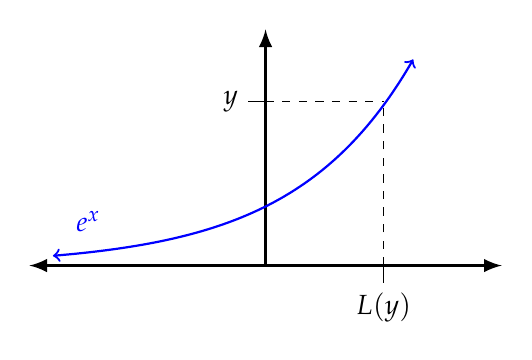
\begin{tikzpicture}[scale=1.5]
        \draw[-latex, very thick] (0, 0) -- (0, 2);
        \draw[latex-latex, very thick] (-2, 0) -- (2, 0);
        \draw[blue, thick, smooth, <->, samples = 100, domain=-1.8:1.25, variable = \x] plot(\x, {0.5*exp(\x)});
        \node[above, text = blue] at (-1.5,0.2) {$e^x$};
        \draw[dashed] (0, 1.39) -- (1, 1.39);
        \draw[dashed] (1, 0) -- (1, 1.39);
        \draw[] (0, 1.39) -- (-0.15, 1.39);
        \node[left] at (-0.15, 1.39) {$y$};
        \draw[] (1, 0) -- (1, -0.15);
        \node[below] at (1, -0.15) {$L(y)$};
    \end{tikzpicture}

    \caption{Plot of $e^x$ and extraction of its inverse $L(y)$.}
    \label{fig53}
\end{figure}

\begin{ntheorem}{: Derivative and Addition Formula}{}
    $L'(y) = \frac{1}{y}$ for $y > 0$ and $L(uv) = L(u) + L(v)$
\end{ntheorem}
\begin{nproof}
    Since $L(E(x)) = x$ by definition, by the chain rule (Theorem \ref{thm:5.5}) we have that:
    \begin{align*}
        L'(E(x))E'(x) = 1 \implies L'(E(x)) = \frac{1}{E(x)}.
    \end{align*}
    Where we use that $E'(x) = E(x)$ in the above implication. Letting $E(x) \mapsto y$, we have that $L'(y) = \frac{1}{y}$ as claimed. For the second claim, consider that for all $u, v > 0$, there exists unique $x, y \in \RR$ (which can be denoted as $\exists ! x, y \in \RR$) such that $E(x) = u, E(y) = v$. Hence:
    \begin{align*}
        L(uv) = L(E(x)E(y)) = L(E(x + y)) = x + y = L(u) + L(v).
    \end{align*}\qed
\end{nproof}

\begin{ncorollary}{}{}
    For $y > 0$, $L(y) = \int_1^y \frac{1}{t}dt$.
\end{ncorollary}
\begin{nproof}
    By the Fundamental Theorem of Calculus (Theorem \ref{thm:6.21}) we have that $\int_1^y \frac{1}{t}dt = L(y) - L(1) = L(y)$. \qed
\end{nproof}

\begin{ntheorem}{}{}
    For $p \in \QQ$, $L(x^p) = pL(x)$.
\end{ntheorem}
\begin{nproof}
    By the addition formula, we have that $L(\frac{1}{x}) + L(x) = L(\frac{1}{x}x) = L(1) = 0$. Hence, $L(\frac{1}{x}) = -L(x)$. Furthermore, by the addition formula, we have that $L(x^n) = nL(x)$ by induction. Furthermore, $L(x^0) = L(1) = 0 = 0L(x)$ which shows that the formula holds for $\NN \cup \set{0}$. Combining the previous facts, we have that:
    \begin{align*}
        nL(x^{\frac{1}{n}}) = L((x^{\frac{1}{n}})^n) = L(x^1) \implies L(x^{\frac{1}{n}}) = \frac{1}{n}L(x)
    \end{align*} 
    We therefore have that for $p = \frac{m}{n}$ with $m, n \in \NN$ that:
    
    \begin{align*}
        L(x^{\frac{m}{n}}) = mL(x^{\frac{1}{n}}) = \frac{m}{n}L(x)
    \end{align*}
    Furthermore,
    \begin{align*}
        L(x^{-\frac{m}{n}}) = L\left(\frac{1}{x^{\frac{m}{n}}}\right) = -L(x^{\frac{m}{n}}) = -\frac{m}{n}L(x)
    \end{align*}
    which shows that the proposed identity holds for all $p \in \QQ$. \qed
\end{nproof}

\begin{ndef}{: Real Exponentials with Arbitrary Base}{}
    For $\alpha \in \RR$, we define $x^\alpha = e^{\alpha \log \alpha}$.
\end{ndef}
\noindent Note that the above definition is equivalen to the definition made in MATH 320 HW3Q1, but it is a much cleaner definition (as we will soon see)!

\begin{ntheorem}{: Generalized Power Rule}{}
    $\od{}{x}x^\alpha = \alpha x^{\alpha -1}$ and hence $x^\alpha$ has antiderivative:
    \begin{align*}
        \begin{cases}
            \frac{1}{\alpha + 1}x^{\alpha + 1} & \text{if $\alpha \neq -1$}
            \\ \log x & \text{if $\alpha = 1$}
        \end{cases}.
    \end{align*}
\end{ntheorem}
\begin{nproof}
    From the definition of $x^\alpha$, we have that:
    \begin{align*}
        \dod{}{x}x^\alpha = \dod{}{x}\left(e^{\alpha \log x}\right) = e^{\alpha \log x} \alpha\frac{1}{x} = \alpha\frac{x^\alpha}{x} = \alpha x^{\alpha - 1}
    \end{align*}
    where in the second equality we use the chain rule and the fact that $L'(y) = \frac{1}{y}$. \qed
\end{nproof}

\begin{ntheorem}{: Subpolynomial Asymptotic Growth}{}
    $\lim_{x \rightarrow \infty} \log x = \infty$, $\lim_{x \rightarrow 0^+} = -\infty$, and $\lim_{x \rightarrow \infty} \frac{\log x}{x^\alpha} = 0$ if $\alpha > 0$.
\end{ntheorem}
\begin{nproof}
    To realize the first two equalities, we first make the observation that $\log(x)$ is (Strictly) monotonically increasing. To see this, let $x_1, x_2 > 0$ and $x_1 < x_2$ and then we have that:
    \begin{align*}
        \log(x_2) - \log(x_1) = \int_0^{x_2} \frac{1}{t}dt - \int_0^{x_1}\frac{1}{t}dt = \int_{x_1}^{x_2}\frac{1}{t}dt > 0
    \end{align*}
    where the bound follows from the fact that $\frac{1}{t} > 0$ for all $t > 0$ and $x_2 - x_1 > 0$. Hence, $\log(x)$ is monotonicaly increasing, and to compute the limits it suffices to compute the limit along a specific choice of sequence that tends to $\infty$ or $0$ respectively. Using that $\linf e^n = \infty$ and $\linf e^{-n} = 0$, we have that:
    \begin{align*}
        \linf \log(e^n) = \linf n\log(e) = \linf n = \infty
    \end{align*}
    \begin{align*}
        \linf \log(e^{-n}) = \linf -n\log(e) = \linf -n = -\infty
    \end{align*}
    so we conclude that $\lim_{x \rightarrow \infty}\log(x) = \infty$ and $\lim_{x \rightarrow 0} \log(x) = -\infty$.

    For the third claim, we let $a > 0$ and $x > 1$. Then:
    \begin{align*}
        \log(x) = \int_1^x \frac{1}{t}dt < \int_1^x t^a\frac{1}{t}dt = \left.\frac{t^a}{a}\right|_{1}^x = \frac{x^a}{a} - \frac{1}{a} < \frac{x^a}{a}
    \end{align*}
    so choosing $a \in (0, \alpha)$ we have that:
    \begin{align*}
        \frac{1}{x^\alpha}\log x < \frac{1}{a}\frac{1}{x^{\alpha - a}} \rightarrow 0 \text{ as } x \rightarrow \infty.
    \end{align*}\qed
\end{nproof}

\subsection{Cosine and Sine}
We have seen that $E(z+w) = E(z)E(w)$ for all $z, w \in \CC$. A natural definition for the complex exponential follows.

\begin{ndef}{: Complex Exponentials}{}
    Given $z \in \CC$, we define:
    \begin{align*}
        e^z = \sum_{n=0}^\infty \frac{z^n}{n!} = E(z)
    \end{align*}
\end{ndef}
\noindent As a remark, note in taking the complex conjugate of $\exp(z)$, we can absorb the conjugation into the argument:
\begin{align*}
    \overline{\exp(z)} = \overline{\sum_{n=0}^\infty \frac{z^n}{n!}} = \sum_{n=0}^\infty \frac{\overline{z}^n}{n!} = \exp(\overline{z})
\end{align*}
\noindent We will now define the trigonometric functions using the complex exponential, and prove the properties that we would expect them to have from our prior geometric notions.

\begin{ndef}{: Cosine and Sine}{}
    Let $x \in \R$. We then define:
    \begin{align*}
        C(x) &= \Re E(ix) = \frac{1}{2}\left[e^{ix} + e^{-ix}\right]
        \\ S(x) &= \Im E(ix) = \frac{1}{2i}\left[e^{ix} - e^{-ix}\right]
    \end{align*}
\end{ndef}

\begin{ntheorem}{: Euler's Formula}{}
    $E(ix) = C(x) + iS(x)$. 
\end{ntheorem}
\begin{nproof}
    The formula is an immediate consequence of the definitions of $C(x), S(x)$. \qed
\end{nproof}
\noindent Note that $C(x), S(x)$ can alternatively (equivalently) be defined as power series:
\begin{align*}
    C(x) &= \frac{1}{2}\sum_{n=0}^\infty \left(\frac{(ix)^n}{n!} + \frac{(-ix)^n}{n!}\right) = \sum_{n=0}^\infty (-1)^n \frac{x^{2n}}{(2n)!}
    \\ S(x) &= \sum_{n=0}^\infty (-1)^n \frac{x^{2n}}{(2n+1)!}
\end{align*}

\begin{ntheorem}{}{}
    Let $x \in \RR$. We then have that:
    \begin{enumerate}
        \item $C(x) = C(-x)$, $C(0) = 1$ and $S(x) = -S(-x)$, $S(0) = 0$.
        \item $C^2(x) + S^2(x) = 1$.
        \item $C'(x) = -S(x)$ and $S'(x) = C(x)$.
    \end{enumerate}
\end{ntheorem}

\begin{nproof}
    \begin{enumerate}
        \item From the definitions of $C$ and $S$, we have:
        \begin{align*}
            C(-x) &= \frac{1}{2}\left[e^{-ix} + e^{ix}\right] = C(x)
            \\ C(0) &= \frac{1}{2}\left[e^{i(0)} + e^{-i(0)}\right] = \frac{1}{2}\left[1 + 1\right] = 1
            \\ -S(-x) &= -\frac{1}{2}\left[e^{-ix} - e^{ix}\right] = \frac{1}{2}\left[e^{ix} - e^{-ix}\right] = S(x)
            \\ S(0) &= \frac{1}{2}\left[e^{i(0)} - e^{-i(0)}\right] = \frac{1}{2}\left[1 - 1\right] = 0
        \end{align*}
        \item Expanding out the expression, we have:
        \begin{align*}
            C^2(x) + S^2(x) &= \frac{1}{4}\left[e^{ix}e^{ix} + 2e^{ix}e^{-ix} + e^{-ix}e^{-ix}\right] - \frac{1}{4}\left[e^{ix}e^{ix} - 2e^{ix}e^{-ix} + e^{-ix}e^{-ix}\right]
            \\ &= e^{ix}e^{-ix}
            \\ &= e^{ix - ix}
            \\ &= e^0
            \\ &= 1
        \end{align*}
        \item Using the linearity of the derivative, and the known result for the derivative of exponentials we have:
        \begin{align*}
            C'(x) &= \frac{1}{2}\left[ie^{ix} - ie^{-ix}\right] = -\frac{1}{2i}\left[e^{ix} - e^{-ix}\right] = -S(x)
            \\ S'(x) &= \frac{1}{2i}\left[ie^{ix} + ie^{-ix}\right] = \frac{1}{2}\left[e^{ix} + e^{-ix}\right] = C(x)
        \end{align*} \qed
    \end{enumerate}
\end{nproof}

\begin{nlemma}{}{}
    There exists $x > 0$ such that $C(x) = 0$. 
\end{nlemma}
\begin{nproof}
    Suppose for the sake of contradiction that $C(x) > 0$ for all $x > 0$. Then, $S$ is strictly increasing as $S' = C$. So, for all $y > x$, we then have that:
    \begin{align*}
        S(x)(y - x) < \int_x^y S(t)dt = -C(y) + C(x) \leq 2
    \end{align*}
    but letting $y \rightarrow \infty$, we get that $\infty \leq 2$ which is a contradiciton. \qed
\end{nproof}

\begin{ndef}{: $\pi$}{}
    Given the above Lemma, $x_0 = \inf\set{x > 0: C(x) = 0}$ exists. In particular, $x_0 > 0$ since $C(0) = 1$ and $C$ is continuous. Then, we define $\pi = 2x_0$. 
\end{ndef}

\begin{ntheorem}{}{}
    $S(\frac{\pi}{2}) = 1$.
\end{ntheorem}
\begin{nproof}
    By the definition of $\pi$, we have that $C(x) > 0$ for $x \in [0, \frac{\pi}{2})$ and $C(\frac{\pi}{2}) = 0$. From the previous theorem we have that $C^2(\frac{\pi}{2}) + S^2(\frac{\pi}{2}) = 1$ so we obtain that $S(\frac{\pi}{2}) = \pm 1$. Since $S(0) = 0$ and $S'(x) = C(x) > 0$ for $x \in [0, \frac{\pi}{2})$, we conclude that $S(\frac{\pi}{2}) = 1$. \qed
\end{nproof}
\noindent Note the implication this result has for $e^{ix}$; using Euler's Formula, we find that:
\begin{align*}
    e^{i\frac{\pi}{2}} = \cos(\frac{\pi}{2}) + i\sin(\frac{\pi}{2}) = 0 + i1 = i
\end{align*}
Therefore:
\begin{align*}
    e^{i\pi} &= \left(e^{i\frac{\pi}{2}}\right)^2 = i^2 = -1
    \\ e^{i\frac{3\pi}{2}} &= \left(e^{i\frac{\pi}{2}}\right)^3 = i^3 = -i
    \\ e^{i2\pi} &= \left(e^{i\frac{\pi}{2}}\right)^4 = i^4 = 1.
\end{align*}
From this we notice the periodicity of $e^{ix}$. 
\begin{ntheorem}{: Periodicity of Trigonometric Functions}{}
    \begin{enumerate}
        \item $e^{x + 2\pi i} = e^x$.
        \item $C(x + 2\pi) = C(x)$.
        \item $S(x + 2\pi) = S(x)$.
    \end{enumerate}
\end{ntheorem}
\begin{nproof}
    \begin{enumerate}
        \item $e^{x + 2\pi i} = e^{x}e^{2\pi i}$ by the addition formula. Then, $e^{2\pi i} = 1$ by the argument above, proving the identity.
        \item Using the above periodicity of $e^{ix}$, we have that $C(x + 2\pi) = \Re(e^{i(x + 2\pi)}) = \Re(e^{ix}) = C(x)$.
        \item $S(x + 2\pi) = \Im(e^{i(x + 2\pi)}) = \Im(e^{ix}) = C(x)$. \qed
    \end{enumerate}
\end{nproof}
\noindent Note that there is a way to relate $S$ and $C$ via a phase shift. We observe that:
\begin{align*}
    S(x + \frac{\pi}{2}) = \Im(e^{i(x + \frac{\pi}{2})}) = \Im(e^{ix}e^{i\frac{\pi}{2}}) = \Im(e^{ix}i) = \Im((C(x) + iS(x))i) = \Im(iC(x) - S(x)) = C(x)
\end{align*}
\noindent We can also generalize this formula to get the familiar trigonometric sum identity.

\begin{ntheorem}{}{}
    $S(x + y) = C(x)S(y) + S(x)C(y)$.
\end{ntheorem}
\begin{nproof}
    Using the definition of $S$ and Euler's Formula, we observe that:
    \begin{align*}
        S(x + y) = \Im(e^{i(x + y)}) 
        &= \Im(e^{ix}e^{iy})
        \\ &= \Im((C(x) + iS(x))(C(y) + iS(y)))
        \\ &= \Im(C(x)C(y) + iS(x)C(y) + iC(x)S(y) - S(x)S(y))
        \\ &= C(x)C(y) - S(x)S(y)
    \end{align*} \qed
\end{nproof}
\noindent As a final remark before moving onto the next section, we observe that $x \mapsto e^{ix}$ is a bijection from $[0, 2\pi)$ onto the unit circle (points $z \in \CC$ with $\abs{z} = 1$). See Rudin for more details.
\begin{figure}[htbp]
    \centering
    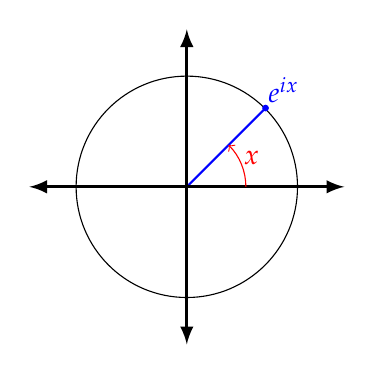
\begin{tikzpicture}
        \draw[blue, thick] (0, 0) -- (1, 1);
        \draw[latex-latex, very thick] (-2, 0) -- (2, 0);
        \draw[latex-latex, very thick] (0, -2) -- (0, 2);
        \draw[smooth] (0, 0) circle (40pt);
        \draw[fill = blue, draw = blue] (1, 1) circle (1pt);
        \draw[->,red] (0.75, 0) arc(0:45:0.75);
        \node[text = red] at (0.82, 0.37) {$x$};
        \node[text = blue] at (1.23, 1.23) {$e^{ix}$};

    \end{tikzpicture}
    
    \caption{Visualization of the map $x \mapsto e^{ix}$ from $[0, 2\pi)$ onto the unit circle in the complex plane.}
    \label{fig55}
\end{figure}


\subsection{The Algebraic Completeness of the Complex Field}

\setcounter{rudin}{7}

\begin{theorem}{The Fundamental Theorem of Algebra}{}
    Let $n \in \NN$, and $a_0, a_1, \ldots, a_n \in \CC$ such that $a_n \neq 0$. Define the polynomial:
    \begin{align*}
        P(z) = a_0 + a_1z + \ldots + a_nz^n
    \end{align*}
    with $z \in \CC$. Then, there exists $z_0 \in \CC$ such that $P(z_0) = 0$. 
\end{theorem}

\begin{ncorollary}{}{}
    By division, $P_n(z)$ has $n$ roots. 
\end{ncorollary}

\begin{nproof}
    Assume WLOG that $a_n = 1$ (this can be realized by dividing out by the original nonzero $a_n$). Let $\mu = \inf_{z \in \CC}\abs{P(z)}$. We wish to show that $\mu = 0$, and that the inf is attained at some $z_0 \in \CC$. 

    We first show that the infimum is attained. The idea of the argument is that for large $z$, $z^n$ grows the most rapidly and hence it dominates. Hence, $\abs{P(z)}$ is large. Hence, the $\inf$ is attained in some compact disk, but since $P$ is continuous, the $\inf$ is therefore obtained somewhere on this compact set. Formally, for $\abs{z} = R$, we have that:
    \begin{align*}
        \abs{P(z)} = \abs{z^n}\abs{\frac{a_0}{z^n} + \frac{a_1}{z^{n-1}} + \ldots + \frac{a_{n-1}}{z} + 1} &\geq \abs{z}^n\left(1 - \frac{\abs{a_0}}{\abs{z}^n} - \frac{\abs{a_1}}{\abs{z}^{n-1}} - \ldots - \frac{\abs{a_{n-1}}}{\abs{z}}\right)
        \\ &= R^n\left(1 - \frac{\abs{a_0}}{\abs{z}^n} - \frac{\abs{a_1}}{\abs{z}^{n-1}} - \ldots - \frac{\abs{a_{n-1}}}{\abs{z}}\right)
    \end{align*}
    We see that this expression goes to infinity as $R \rightarrow \infty$. Hence, $\abs{P(z)} \geq \mu + 1$ if $\abs{z} \geq R_0$ for some $R_0 > 0$. As $\abs{P}$ is continuous, and $\abs{z} \leq R_0$ is a compact subset of $\CC$, $\mu$ is attained somewhere on the subset by the Extreme Value Theorem (Theorem \ref{thm:4.16}). Therefore, $\mu = \abs{P(z_0)}$ for some $z_0$ with $\abs{z_0} \leq R_0$. 

    Next, we show that $\mu = 0$. Suppose (for the sake of contradiction) that $\mu > 0$ and hence $P(z_0) \neq 0$. Let $Q(z) = \frac{P(z_0 + z)}{P(z_0)}$. Then $Q(0) = 1$, so:
    \begin{align*}
        Q(z) = 1 + b_kz^k + \ldots + b_nz^n
    \end{align*}
    where $b_k$ is the first nonzero coeffient. Furthermore, we see that $\abs{Q(z)} = \frac{\abs{P(z_0 + z)}}{\mu} \geq 1$ for all $z \in \CC$ (as $\mu$ is the infimum). We will now derive a contradiction by looking at small $z$ (where $z^k > z^{k+1} > \ldots > z^n$). We consider that:
    \begin{align*}
        \abs{Q(z)} \leq \abs{1 + b_kz^k} + \sum_{m=k+1}^n \abs{b_m}\abs{z^m}
    \end{align*}
    We want to choose $z$ small enough such that the first term in the above expression is less than $1$ and the others are negligeble. To this end, let us write $bk = \frac{b_k}{\abs{b_k}}\abs{b_k} = e^{it_1}\abs{b_k}$ for some $t_1 \in \RR$. Then, let $t = \frac{-t_1 + \pi}{k}$ so $t_1 = -kt + \pi$. We then have that $b_k = -e^{-itk}\abs{b_k}$ (where the minus sign comes from $e^{i\pi}$). Choose $z = re^{it}$ with $r > 0$. Then, $z^k = r^ke^{itk}$ and $b_kz^k = -e^{-itk}\abs{b_k}r^ke^{itk} = -r^k\abs{b_k} < 0$. Let us choose $r$ small enough so that $\abs{b_k}r^k < 1$ is satisfied. We then have that:
    \begin{align*}
        \abs{1 + b_kz^k} = \abs{1 - \abs{b_k}r^k} = 1 - \abs{b_k}r^k
    \end{align*}
    so therefore:
    \begin{align*}
        \abs{Q(z)} \leq 1 - \abs{b_k}r^k + \sum_{m=k+1}^n \abs{b_m}r^k = 1 - r^k\left(\abs{b_k} - r\abs{b_{k+1}} - \ldots - r^{n-k}\abs{b_n}\right)
    \end{align*}
    where $\left(\abs{b_k} - r\abs{b_{k+1}} - \ldots - r^{n-k}\abs{b_n}\right) > 0$. Hence $\abs{Q(z)} < 1$, which is a contradiction. We conclude that $\abs{P(z_0)} = 0$. \qed
\end{nproof}

\subsection{Fourier Series}
\section[Functions of Several Variables]{\hyperlink{toc}{Functions of Several Variables}}

\end{document}